\documentclass[lang=cn,10pt,thmcnt=section]{elegantbook}
\usepackage{graphicx}
\usepackage{float}
\usepackage{esint}
\usepackage{mathtools}
\usetikzlibrary{math}
\usepackage{tikz}
\usepackage{wrapfig}
\usepackage{tikz-3dplot}
\usetikzlibrary{decorations.markings}
\usepackage{ifthen}
\title{微分几何}



\author{黄}
\date{\today}




\setcounter{tocdepth}{3}


\cover{cover.jpg}

% 本文档命令
\usepackage{array}
\newcommand{\ccr}[1]{\makecell{{\color{#1}\rule{1cm}{1cm}}}}
\newcommand{\dd}{\mathrm{d}}
\renewcommand{\vec}[1]{\mathbf{#1}}
% 修改标题页的橙色带
% \definecolor{customcolor}{RGB}{32,178,170}
% \colorlet{coverlinecolor}{customcolor}
\begin{document}
	
	\maketitle
	\frontmatter
	
	\tableofcontents
	
	\mainmatter
\chapter{预备知识}
\section{向量空间}
\begin{definition}[同向]
    我们称线段 $AB$ 和 $A'B'$ 同向,若以下情况成立:
    \begin{enumerate}
        \item $A = A'$,则 $ABB'$ 共线且 $B$ 和 $B'$ 在 $A$ 的同一侧;
        \item 若 $A \neq A'$,则连接 $AA'$ 得到直线 $l$,一定能在 $l$ 上再取 $D$,使 $A$ 和 $A'$ 在 $D$ 的同一侧且 $\angle DAB = \angle DA'B'$。
    \end{enumerate}
\end{definition}

\begin{definition}[向量集]
    我们在 $\mathbb{E}^3 \times \mathbb{E}^3$ 上定义 $\sim$:
    \[
    (A, B) \sim (C, D) \iff AB \text{ 和 } CD \text{ 等长度且同向。}
    \]
    则记 $\mathbb{V} = \mathbb{E}^3 \times \mathbb{E}^3 / \sim$ 为向量集,$\mathbb{V}$ 中元素称为向量。
\end{definition}
\begin{definition}[加法]
 三角法则
\end{definition}

\begin{remark}
    加法需要验证定义,因为事实上我们在强行定义
\[
[\overrightarrow{OA}] + [\overrightarrow{AB}] = [\overrightarrow{OB}]
\]
\end{remark}
\begin{definition}[数乘]
    \[
m : \mathbb{R} \times \mathbb{V} \rightarrow \mathbb{V}
\]
\[
(\lambda, \vec{a}) \mapsto \lambda \vec{a}
\]
\end{definition}

\begin{definition}
    规定 $\lambda \vec{a}$ 为满足以下条件的向量:
    \begin{enumerate}
        \item 若 $\lambda = 0$ 或 $\vec{a} = \vec{0}$,则 $\lambda \vec{a} = \vec{0}$;
        \item 若 $\lambda > 0$,则 $\lambda \vec{a}$ 和 $\vec{a}$ 同向;
        \item 若 $\lambda < 0$,则 $\lambda \vec{a}$ 和 $\vec{a}$ 反向;
        \item $|\lambda \vec{a}| = |\lambda| \cdot |\vec{a}|$。
    \end{enumerate}
\end{definition}

\begin{proposition}
    $(\mathbb{V}, +, m)$ 构成一个实数域上的线性空间,故而称之为向量空间。

    \begin{equation*}
        \begin{split}
            \lambda (\mu \vec{u}) &= (\lambda \mu) \vec{u}\\
            1 \cdot \vec{u} &= \vec{u}\\  
            (\lambda + \mu) \vec{u} &= \lambda \vec{u} + \mu \vec{u}\\
            \lambda (\vec{u} + \vec{v})& = \lambda \vec{u} + \lambda \vec{v}
        \end{split}
     \end{equation*}
\end{proposition}
    
 $\mathbb{V}$上有点乘和叉乘两个运算

\begin{definition}[点积]
    \begin{itemize}
        \item $\cdot : \mathbb{V} \times \mathbb{V} \rightarrow \mathbb{R}$
        \item $(\vec{u}, \vec{v}) \mapsto \vec{u} \cdot \vec{v}$
        \item $\vec{u} \cdot \vec{v} = |\vec{u}| \cdot |\vec{v}| \cdot \cos \theta$,$\theta$ 为两者夹角
        \item 若其中有 $\vec{0}$,且强行规定 $\vec{0} \cdot \vec{v} = 0$
    \end{itemize}
\end{definition}

\begin{definition}[叉积]
    \begin{itemize}
        \item $\times : \mathbb{V} \times \mathbb{V} \rightarrow \mathbb{V}$
        \item $(\vec{u}, \vec{v}) \mapsto \vec{u} \times \vec{v}$
    \end{itemize}
    
    $\vec{u} \times \vec{v}$ 由以下公式唯一决定:
    \begin{enumerate}
        \item 若 $\vec{u}, \vec{v}$ 共线,规定 $\vec{u} \times \vec{v} = \vec{0}$
        \item 不然则:
        \begin{enumerate}
            \item $|\vec{u} \times \vec{v}| = |\vec{u}| |\vec{v}| \sin \theta$
            \item $\vec{u} \times \vec{v}$ 同时和 $\vec{u}, \vec{v}$ 垂直
            \item $\{\vec{u}, \vec{v}, \vec{u} \times \vec{v}\}$ 满足右手法则
        \end{enumerate}
    \end{enumerate}

\end{definition}

\begin{definition}[内积]
    设 $W$ 为 $\mathbb{C}$ 上的线性空间,称 $<\cdot,\cdot> : W \times W \rightarrow \mathbb{C}$ 为一个内积,若其满足:
    \begin{enumerate}
        \item 共轭对称性:$<u,v> = \overline{<v,u>}$ ($<v,u>$)
        \item 正定性:$\forall u, <u,u> \geq 0$,且 $<u,u> = 0 \Leftrightarrow u = 0$
        \item 线性:$<\lambda u + \mu v, w> = \lambda <u,w> + \mu <v,w>$
    \end{enumerate}
    命题 $(V, \cdot)$ 构成内积空间。(难点:线性)
    \end{definition}
    
    \begin{definition}[李括号]
    设 $W$ 为线性空间,称 $[ \cdot, \cdot ] : W \times W \rightarrow W$ 为一个李代数,若其满足线性,我们称其为一个李括号,若还有:
    \begin{enumerate}
        \item 反对称性:$[u,v] = -[v,u]$
        \item Jacobi恒等式:$[u,[v,w]] + [v,[w,u]] + [w,[u,v]] = 0$
    \end{enumerate}
    例:令 $W$ 为全体 $n \times n$ 矩阵,命题 $(V, \cdot)$ 是一个李代数。
\end{definition}
\begin{definition}[基和坐标]
    我们称不共面的三个向量构成 $\mathbb{V}$ 的一组基。我们称 $\{e_1, e_2, e_3\}$ 为单位正交基。若
\[
e_i \cdot e_j = \delta_{ij} = 
\begin{cases} 
0, & i \neq j \\
1, & i = j 
\end{cases}
\]

设 $\{e_1, e_2, e_3\}$ 为基,$\forall \vec{a} \in \mathbb{V}$,若
\[
\vec{a} = a_1 e_1 + a_2 e_2 + a_3 e_3
\]
记 $\vec{a} = (a_1, a_2, a_3)$ 称为坐标。
\end{definition}
\begin{proposition}[点积、叉积、混合积的公式]
设 $\{e_1, e_2, e_3\}$ 为单位正交基,$\vec{a} = (a_1, a_2, a_3)$,$\vec{b} = (b_1, b_2, b_3)$。
\begin{itemize}
    \item 点积:$\vec{a} \cdot \vec{b} = a_1b_1 + a_2b_2 + a_3b_3$。
    \item 若 $\{e_1, e_2, e_3\}$ 还满足右手法则,则
    \[
    \vec{a} \times \vec{b} = 
    \begin{vmatrix}
    e_1 & e_2 & e_3 \\
    a_1 & a_2 & a_3 \\
    b_1 & b_2 & b_3
    \end{vmatrix}
    \]
    \item 混合积:$[\vec{a}, \vec{b}, \vec{c}] \triangleq (\vec{a} \times \vec{b}) \cdot \vec{c} = 
    \begin{vmatrix}
    a_1 & a_2 & a_3 \\
    b_1 & b_2 & b_3 \\
    c_1 & c_2 & c_3
    \end{vmatrix}$。
\end{itemize}
\end{proposition}
\begin{definition}[坐标系]
    若 $\{e_1, e_2, e_3\}$ 为基,取定 $O \in \mathbb{E}^3$,则 $\mathbb{E}^3$ 中每一点都有唯一的坐标。对 $\forall P \in \mathbb{E}^3$,若 $\overrightarrow{OP} = x e_1 + y e_2 + z e_3$,则称 $P = (x, y, z)$ 为其坐标。记 $I = \{O; e_1, e_2, e_3\}$ 为一个坐标系。
\end{definition}
\section{向量值函数}
我们称到 $\mathbb{E}^3$ 的函数为向量值函数。

\textbf{曲线:} $[a,b] \xrightarrow{\gamma} \mathbb{E}^3, \quad t \mapsto \gamma(t) = (x(t), y(t), z(t))$。

\textbf{曲面:} $D \subset \mathbb{R}^2 \xrightarrow{\gamma} \mathbb{E}^3$.$(u,v) \mapsto \gamma(u,v) = (x(u,v), y(u,v), z(u,v))$。

\begin{enumerate} 
    \item 我们经常将曲线和曲面的像和映射本身不加区分。
    \item 有时为了强调值为向量,也记为 $\vec{\gamma}(t)$,$\vec{\gamma}(u,v)$。
\end{enumerate}

称 $\vec{r}(t)$ 是 $C^k$ 的,若每个分量都是 $C^k$ 的。

\begin{definition}
    $\vec{r}'(t) = (x'(t), y'(t), z'(t))$.
    \[
    \int_a^b \vec{r}(t) \, dt = \left( \int_a^b x(t) \, dt, \int_a^b y(t) \, dt, \int_a^b z(t) \, dt \right).
    \]
\end{definition}

\begin{proposition}[Leibniz法则]
    \begin{enumerate}
        \item $\left( \vec{a}(t) \cdot \vec{b}(t) \right)' = \vec{a}'(t) \cdot \vec{b}(t) + \vec{a}(t) \cdot \vec{b}'(t)$.
        \item $\left( \vec{a}(t) \times \vec{b}(t) \right)' = \vec{a}'(t) \times \vec{b}(t) + \vec{a}(t) \times \vec{b}'(t)$.
        \item $[a, b, c]'== [a', b, c] + [a, b', c] + [a, b, c'].$
    \end{enumerate}
\end{proposition}

\begin{definition}[nabla算子]
    \[
\nabla = \left( \frac{\partial}{\partial x}, \frac{\partial}{\partial y}, \frac{\partial}{\partial z} \right) \quad \text{称为一个向量值的算子。}
\]
\end{definition}
取 $f: \mathbb{R}^3 \rightarrow \mathbb{R}$。
\begin{definition}[梯度]
    定义 $\nabla f = (f_x, f_y, f_z)$ 称为 $f$ 的梯度。
    \end{definition}
    
    取 $\vec{F}: \mathbb{R} \rightarrow \mathbb{R}^3$,$\vec{F}(t) = (F_1(t), F_2(t), F_3(t))$。
    
    \begin{definition}[散度]
    定义 $\nabla \cdot \vec{F} = (F_1)_x + (F_2)_y + (F_3)_z$,称为 $\vec{F}$ 的散度。
    \end{definition}
    
    \begin{definition}[旋度]
    $\nabla \times \vec{F} = \left| \begin{matrix}
        e_1&		e_2&		e_3\\
        \frac{1}{\partial x}&		\frac{1}{\partial y}&		\frac{1}{\partial z}\\
        F_1&		F_2&		F_3\\
    \end{matrix} \right|$,称为 $\vec{F}$ 的旋度。
    \end{definition}






\section{几何变换}
\subsection{仿射变换}
\begin{definition}[线性变换]
    我们称 $\phi: X \rightarrow X$ 为一个 $X$ 上的变换,若其为一一对应。
\end{definition}
\begin{definition}[仿射变换]
    设 $\phi: \mathbb{E}^3 \rightarrow \mathbb{E}^3$ 为变换,称其为一个仿射变换,若其将直线映为直线。
\end{definition}
\begin{proposition}
    \begin{enumerate}
        \item 所有仿射变换在复合下构成一个变换群。(难点:逆)
        \item 中将平面映成平面。
        \item 中将一对相交直线映成相交直线。
        \item 中将平行直线映成平行直线。
        \item 中将平行四边形映成平行四边形。
    \end{enumerate}
\end{proposition}

\begin{definition}[诱导映射]
    设 $\phi: \mathbb{E}^3 \rightarrow \mathbb{E}^3$ 仿射,其诱导一个 $\widehat{\phi}:V \rightarrow V$ 的映射。
    \[
    \begin{aligned}
        &\widehat{\phi}: V \rightarrow V \\
        &\vec{a} = \overrightarrow{PQ} \mapsto \widehat{\phi}(\vec{a}) = \overrightarrow{\phi(P)\phi(Q)}
    \end{aligned}
    \]
    我们通常不区分 $\phi$ 和 $\widehat{\phi}$。
\end{definition}


\begin{theorem}
    诱导映射是线性映射,即有
\[
\widetilde{\phi}(\lambda \vec{a} + \mu \vec{b}) = \lambda \widetilde{\phi}(\vec{a}) + \mu \widetilde{\phi}(\vec{b}).
\]
\end{theorem}
\begin{lemma}
    设 $\phi: \mathbb{E}^3 \rightarrow \mathbb{E}^3$ 为仿射变换,
    \begin{enumerate}
        \item 若 $ABC$ 共线,则 $\phi$ 保持其共线性。$(A, B; C) = \frac{\overrightarrow{AC}}{\overrightarrow{CB}}$。我们称 $P \in \mathbb{E}^3$ 为其不动点,若 $\phi(P) = P$。
        \item 若 $\phi$ 有两个不动点 $A, B$,则 $\phi$ 保持整条直线 $AB$ 不动。
        \item 若 $\phi$ 有三个不共线不动点,则 $\phi$ 保持平面不动。
        \item 若 $\phi$ 有四个不共面不动点,则 $\phi = \text{id}$。
    \end{enumerate}
\end{lemma}
\begin{proof}

    (1)设$\lambda=(A, B; C) = \frac{\overrightarrow{AC}}{\overrightarrow{CB}} \Leftrightarrow \overrightarrow{AC}=\lambda\overrightarrow{CB}$
    $$
\text{那么}\left. \begin{array}{r}
	\phi \left( \overrightarrow{AC} \right) =\overrightarrow{\phi \left( A \right) \phi \left( C \right) }\\
	\phi \left( \overrightarrow{\lambda CB} \right) =\lambda \phi \left( \overrightarrow{CB} \right) =\lambda \overrightarrow{\phi \left( C \right) \phi \left( B \right) }\\
\end{array} \right\} \Rightarrow \left( \phi \left( A \right) ,\phi \left( B \right) ;\phi \left( C \right) \right) =\left( A,B;C \right) 
$$

    (2)连接 $AB$ 得到直线 $l$,取 $l$ 上另一点 $C$.
    $$
\text{由}\left( 1 \right) ,A,B\text{不动}\begin{cases}
	\overrightarrow{AC}=\lambda \overrightarrow{CB}\\
	\overrightarrow{\phi \left( A \right) \phi \left( C \right) }=\lambda \overrightarrow{\phi \left( C \right) \phi \left( B \right) }\Leftrightarrow \overrightarrow{A\phi \left( C \right) }=\lambda \overrightarrow{\phi \left( C \right) B}\\
\end{cases}\Rightarrow \phi \left( C \right) =C
$$

    (3)三条直线都不动

    $$
\left. \begin{array}{r}
	AB\text{不动}\Rightarrow AB\text{连线之间任意一个点}Y\text{都不动}\\
	BC\text{不动}\Rightarrow BC\text{连线之间任意一个点}Z\text{都不动}\\
\end{array} \right\} \Rightarrow YZ\text{不动}\Rightarrow YZ\text{连线上任意一点}X\text{不动}
$$

由任意性,平面保持不动

    (4)四个面都不动,我们任取一个$X$,做过其的直线与其中两个平面相交,则$X$不动,为恒等映射

    
\end{proof}


\begin{theorem}[仿射变换基本定理 Part 1]
    设 $\{A, B, C, D\}$,$\{A', B', C', D'\}$ 为两个不共面的四点组,则存在唯一的仿射变换 $\phi$ 使得
    \[
    \phi(A) = A', \quad \phi(B) = B', \quad \phi(C) = C', \quad \phi(D) = D'.
    \]
    \end{theorem}
    
    \begin{proof}
    $\{A, B, C, D\}$ 不共面 $\Leftrightarrow \mathbb{I}' = \{A'; \overrightarrow{A'B'}, \overrightarrow{A'C'}, \overrightarrow{A'D'}\}$ 为一个坐标系。
    \end{proof}
    
    直接定义中:$\mathbb{E}^3 \rightarrow \mathbb{E}^3$ $(x, y, z)_{\mathbb{I}} \mapsto (x, y, z)_{\mathbb{I}'}$
    
    \begin{itemize}
        \item 利用坐标系的一一对应可知中良定义且双射。
        \item $\phi(A) = A'$ 因为 $(0,0,0)_{\mathbb{I}} \mapsto (0,0,0)_{\mathbb{I}'}$。
        \item 同理,四个点都可验证。
        \item 线性,因为 $A, B, C$ 共线 $\Leftrightarrow \exists \lambda \in \mathbb{R}$ 使 $\overrightarrow{OC} = \lambda \overrightarrow{OA} + (1-\lambda) \overrightarrow{OB}$.
        \item 唯一性,若还有中满足所有要求。
        \item 考察 $\phi^{-1}\psi$ 中有四个不共面的不动点 $\Rightarrow \phi^{-1}\psi$ 为 $\text{id}$ $\Rightarrow \phi = \psi$.
    \end{itemize}
    
    \begin{theorem}[仿射变换基本定理 Part 2]
    仿射变换和坐标变换一一对应。
    \begin{enumerate}
        \item 设 $\{O; e_1, e_2, e_3\}$,$\{O'; e_1', e_2', e_3'\}$ 为两个坐标系,且存在仿射变换中使 $\phi(O) = O'$,$\phi(e_i) = e_i'$.
        \item 若 $\phi$ 为仿射变换,且 $\{O; e_1, e_2, e_3\}$ 为坐标系,则 $\{\phi(O); \phi(e_1), \phi(e_2), \phi(e_3)\}$ 也是一个坐标系。
    \end{enumerate}
    \end{theorem}
    \begin{proof}
        \begin{enumerate}
            \item 即 Part 1,只需将 $\{O; e_1, e_2, e_3\}$ 理解为 $\{O, A, B, C\}$.
            \item 即证 $\{\phi(e_1), \phi(e_2), \phi(e_3)\}$ 线性无关,若有 $\lambda, \mu, \nu \in \mathbb{R}$,使
            \[
            \lambda \phi(e_1) + \mu \phi(e_2) + \nu \phi(e_3) = \overrightarrow{0}.
            \]
            \[
            \Leftrightarrow \phi(\lambda e_1 + \mu e_2 + \nu e_3) = \overrightarrow{0}.
            \]
            \[
            \Leftrightarrow \lambda e_1 + \mu e_2 + \nu e_3 = \overrightarrow{0} + \{e_1, e_2, e_3\} \text{ 为基}
            \]
            \[
            \Rightarrow \lambda = \mu = \nu = 0 \quad \text{故而 } \{\phi(0), \phi(e_1), \phi(e_2), \phi(e_3)\} \text{ 为坐标系}.
            \]
        \end{enumerate}
    \end{proof}

    \begin{theorem}[仿射变换的坐标]\label{thm:affine_coordinates}
        设 $\phi: \mathbb{E}^3 \rightarrow \mathbb{E}^3$,取 $\{O; e_1, e_2, e_3\}$,若 $P = (x, y, z)$,则有以下公式:
        \[
        \begin{pmatrix}
        x' \\
        y' \\
        z'
        \end{pmatrix}
        =
        A
        \begin{pmatrix}
        x \\
        y \\
        z
        \end{pmatrix}
        + \mathbf{c}
        \]
        其中 $A \in \text{GL}_3(\mathbb{R})$,称为过渡矩阵,$\mathbf{c}$ 为列向量,称为平移向量。
        \end{theorem}
        
        \begin{proof}
        由基本定理可知,$\{\phi(O), \phi(e_1), \phi(e_2), \phi(e_3)\}$ 也是一个坐标系。那么必然存在 $A \in \text{GL}_3(\mathbb{R})$,使得
        \[
        (\phi(e_1), \phi(e_2), \phi(e_3)) = (e_1, e_2, e_3) A
        \]
        \[
        P = (x, y, z) \Leftrightarrow \overrightarrow{OP} = x e_1 + y e_2 + z e_3 = (e_1, e_2, e_3) \begin{pmatrix} x \\ y \\ z \end{pmatrix}
        \]
        \[
        \Rightarrow \phi(\overrightarrow{OP}) = \phi(\overrightarrow{O}) + \phi(\overrightarrow{OP}) = (\phi(e_1), \phi(e_2), \phi(e_3)) \begin{pmatrix} x \\ y \\ z \end{pmatrix} = (e_1, e_2, e_3) A \begin{pmatrix} x \\ y \\ z \end{pmatrix}
        \]
        再设 $\overrightarrow{O\phi(O)} = (e_1, e_2, e_3) \begin{pmatrix} c_1 \\ c_2 \\ c_3 \end{pmatrix} = (e_1, e_2, e_3) \mathbf{C}$\text{(两式相加即证)}
        \end{proof}
    \subsection{等距变换}
    \begin{definition}[等距变换]
        设 $\phi: \mathbb{E}^3 \to \mathbb{E}^3$,$Q \in \mathbb{E}^3$,$\mathcal{L}$ 为 $\mathbb{E}^3$ 上的线性变换,若
        \[
        d(\phi(P), \phi(Q)) = |\overrightarrow{PQ}|
        \]
        称 $\phi: \mathbb{E}^3 \to \mathbb{E}^3$ 为等距变换,若有 $d(\phi(P), \phi(Q)) = d(P, Q)$,则等距变换一定是仿射变换。
        \end{definition}
        
        \begin{proposition}
        设 $\phi$ 为等距,则
        \begin{enumerate}
            \item $\forall \vec{a} \in \mathbb{R}^3$,$|\phi(\vec{a})| = |\vec{a}|$
            \item $\forall \vec{a}, \vec{b} \in \mathbb{R}^3$,$\phi(\vec{a}) \cdot \phi(\vec{b}) = \vec{a} \cdot \vec{b}$
            \item $4 \vec{a} \cdot \vec{b} = |\vec{a} + \vec{b}|^2 - |\vec{a} - \vec{b}|^2$
        \end{enumerate}
        \end{proposition}
    
        \begin{definition}[直角坐标系]
            我们称 $\{O; e_1, e_2, e_3\}$ 为直角坐标系,若 $\{e_1, e_2, e_3\}$ 单位正交。
            \end{definition}
            
            \begin{definition}[等距变换]
            等距变换和直角坐标系之间的变换一一一对应。
            \end{definition}
            
            \begin{proof}
            证明:
            \begin{enumerate}
                \item 即补证:$\{\phi(e_1), \phi(e_2), \phi(e_3)\}$ 为单位正交基。
                \begin{equation*}
                \phi(e_i) \cdot \phi(e_j) = e_i \cdot e_j = \delta_{ij}
                \end{equation*}
                \item 若两者皆直角坐标系,设 $\overrightarrow{PQ} = (x, y, z)_{\mathbb{I}} \Leftrightarrow \phi(\overrightarrow{PQ}) = (x, y, z)_{\mathbb{I}'}$。
                \begin{equation*}
                \Rightarrow \phi(\overrightarrow{PQ}) = (x, y, z)_{\mathbb{I}'} = (x, y, z)_{\mathbb{I}} \phi(O)
                \end{equation*}
                \begin{equation*}
                \Rightarrow |\overrightarrow{PQ}| = \sqrt{x^2 + y^2 + z^2}
                \end{equation*}
            \end{enumerate}
            \end{proof}
            
            \begin{proposition}
            设 $\phi: \mathbb{E}^3 \rightarrow \mathbb{E}^3$ 为等距变换,其对应的公式为
            \begin{equation}
            \begin{pmatrix}
            x' \\
            y' \\
            z'
            \end{pmatrix}
            = A
            \begin{pmatrix}
            x \\
            y \\
            z
            \end{pmatrix}
            + C
            \end{equation}
            其中 $A \in O_3(\mathbb{R}) = \{A \in GL_3(\mathbb{R}) \mid AA^T = E_3\}$,$C$ 为列向量。
            \end{proposition}
\subsection{刚体运动}
我们只需讲清楚基的定向。


\begin{proposition}
    $\{\vec{a}, \vec{b}, \vec{c}\}$ 共面 $\Leftrightarrow [\vec{a}, \vec{b}, \vec{c}] = 0$
\end{proposition}
\begin{proof}
    \begin{itemize}
        \item[$(\Rightarrow)$] 若 $\vec{a}, \vec{b}, \vec{c}$ 共面且线性相关,
        \[
        \vec{c} = \lambda \vec{a} + \mu \vec{b}.
        \]
        则
        \[
        [\vec{a}, \vec{b}, \vec{c}] = (\vec{a} \times \vec{b}) \cdot (\lambda \vec{a} + \vec{b}) = 0.
        \]
        
        \item[$(\Leftarrow)$] 若 $[\vec{a}, \vec{b}, \vec{c}] = 0$,假设 $\vec{a}, \vec{b}$ 不共线,否则命题自动成立。
        \[
        \{\vec{a}, \vec{b}, \vec{a} \times \vec{b}\} \text{ 构成一组基。}
        \]
        \[
        \vec{c} = \lambda \vec{a} + \vec{b} + \vec{a} \times \vec{b}.
        \]
        \[
        [\vec{a}, \vec{b}, \vec{c}] = 0
        \]
        \[
        (\vec{a} \times \vec{b}) \cdot (\lambda \vec{a} + \vec{b} + \vec{a} \times \vec{b}) = 0.
        \]
        \[
        \gamma |\vec{a} \times \vec{b}|^2 = 0.
        \]
        但 $\vec{a}, \vec{b}$ 不共线,
        \[
        \gamma = 0 \Rightarrow \vec{c} = \lambda \vec{a} + \vec{b} \Rightarrow \text{三者共面}.
        \]
    \end{itemize}
    \end{proof}
\begin{definition}[左手系和右手系]
    设 $\{e_1, e_2, e_3\}$ 为基,
    \begin{equation}
    [e_1, e_2, e_3] < 0 \quad \text{为左手系,} \quad > 0 \quad \text{为右手系。}
    \end{equation}
\end{definition}
\begin{definition}[定向]
    称 $[e_1, e_2, e_3]$ 为基的定向。
\end{definition}
\begin{definition}[保定向]
    设 $\phi: \mathbb{E}^3 \rightarrow \mathbb{E}^3$ 为仿射变换,若其将右手系映为右手系,则称其为保定向的,否则为反定向的。
\end{definition}
\begin{theorem}[刚体运动的坐标]
    其对应公式形如:
    \begin{equation}
    \begin{pmatrix}
    x' \\
    y' \\
    z'
    \end{pmatrix}
    = A
    \begin{pmatrix}
    x \\
    y \\
    z
    \end{pmatrix}
    + C
    \end{equation}
    其中 $A \in SO_3(\mathbb{R}) = \{A \in O_3(\mathbb{R}) \mid \det A = 1\}$。
\end{theorem}
\begin{proof}
    注意到:
    \begin{equation}
    (\phi(e_1), \phi(e_2), \phi(e_3)) = (e_1, e_2, e_3) A
    \end{equation}
    两边取行列式:
    \begin{equation}
    \det A = 1 \quad \text{(保定向)}
    \end{equation}
\end{proof}

\begin{theorem}[刚体运动分解]
    刚体运动 = $A + C$ = 旋转变换 + 平移变换。
\end{theorem}

\begin{definition}[几何量]
    若某量和坐标选取无关,且在刚体运动下不变,则称此量为几何量。
\end{definition}
    
\begin{itemize}
    \item 例:长度、面积、曲率、挠率、Frenet 标架等。
\end{itemize}

\chapter{曲线论}
\section{曲线和正则曲线}
\begin{definition}[曲线]
    设 $E \subset \mathbb{R}$ 为 $\mathbb{R}$ 中的连通集。我们称 $\gamma: E \subset \mathbb{R} \rightarrow \mathbb{E}^3$ 为 $\mathbb{E}^3$ 中的一条曲线,连续映射,其中 $t \mapsto \gamma(t) = (x(t), y(t), z(t))$ 为 $\mathbb{E}^3$ 中的一条曲线。
\end{definition}
\begin{remark}
    一般强调起点经过时取 $E = [a, b]$。
\end{remark}
\begin{definition}[正则曲线]
    我们称一条曲线 $\gamma$ 在 $t_0$ 处正则,若 $\gamma$ 在 $t_0$ 处可微且 $\gamma'(t_0) \neq \vec{0}$。我们称 $\gamma: E \subset \mathbb{R} \rightarrow \mathbb{E}^3$ 为一条正则曲线,若
    \begin{enumerate}
        \item $x, y, z \in C^3(E)$
        \item $\gamma$ 在 $E$ 的每一点均正则。
    \end{enumerate}
\end{definition}
\begin{theorem}
    设 $E, F \subseteq \mathbb{R}$ 为两个向量空间,$r: E \rightarrow E^3$ 为正则曲线。
    
    若存在映射 $f: F \rightarrow E$,连续映射 $u \mapsto f(u) = t$,双射?
    
    那么我们可定义一条 $F$ 上的曲线
\begin{align*}
r \circ f: F &\longrightarrow E^3 \\
u &\longmapsto r \circ f(u) = (x_f(u), y_f(u), z_f(u)).
\end{align*}
\end{theorem}
我们称 $t = f(u)$ 为一个正则换元,若其满足:
\begin{enumerate}
    \item $f \in C^3(F)$.
    \item $f'(u) \neq 0, \forall u \in F$.
\end{enumerate}

\begin{theorem}\label{thm:regular_parameter}
曲线的正则性和正则换元无关。
\end{theorem}
\begin{proof}
    \begin{enumerate}
        \item $f \in C^3 + x, y, z \in C^3 \Rightarrow x \circ f, \ldots, z \circ f \in C^3$
        \item $ (r \circ f)'(u) = (x \circ f(u), y \circ f(u), z \circ f(u))' $
    \end{enumerate}
    
    \[
    (f'(u) \cdot x'(t), f'(u) \cdot y'(t), f'(u) \cdot z'(t)) = f'(u) \cdot r'(t) \neq \vec{0}
    \]
\end{proof}

\begin{remark}
    我们可以定义等价关系 $r_1 \sim r_2 \Leftrightarrow$ 若存在正则换元 $f$ 使 $r_1 = r_2 \circ f$。

事实上我们认为的正则曲线是 $\sim$ 下的等价类。


\end{remark}

\begin{example}
    正螺线

    \tdplotsetmaincoords{60}{120}
    \begin{figure}[H]
        \centering
        \begin{tikzpicture}[tdplot_main_coords,scale=3]
	% Parametric equations of the surface
	\tikzmath{function equis(\u,\v) {return \u*cos(\v r);};}
	\tikzmath{function ye(\u,\v) {return \u*sin(\v r);};}
	\tikzmath{function zeta(\u,\v) {return \c*\v;};}
	% Parameter for the function
	\pgfmathsetmacro{\c}{1.0/(2.0*pi)}
	% Domain for the graph
	\pgfmathsetmacro{\uunoi}{-0.75}
	\pgfmathsetmacro{\uunof}{0.75}
	\pgfmathsetmacro{\vi}{-2.0*pi}
	\pgfmathsetmacro{\vf}{2.0*pi}
	\pgfmathsetmacro{\step}{\uunoi+\vf/500}
	\pgfmathsetmacro{\stepn}{\vi+\vf/500}
	% The graph of the function
	\foreach \u in {\uunoi,\step,...,\uunof}{
		\draw[cyan,thick,opacity=0.25] plot[domain=\vi:\vf,smooth,variable=\v] ({equis(\u,\v)},{ye(\u,\v)},{zeta(\u,\v)});
	}
	\foreach \v in {\vi,\stepn,...,\vf}{
		\draw[cyan,thick,opacity=0.25] plot[domain=\uunoi:\uunof,smooth,variable=\u] ({equis(\u,\v)},{ye(\u,\v)},{zeta(\u,\v)});
	}
\end{tikzpicture}
    \end{figure}

\[
r(t) = (a\cos t, a\sin t, bt), \quad t \in (-\infty, +\infty) \quad (a > 0)
\]
\[
a(\cos t, \sin t, 0) + b(0, 0, t) \Rightarrow \text{正则}
\]
\[
r'(t) = (-a\sin t, a\cos t, b) \Rightarrow |r'(t)| = \sqrt{a^2 + b^2} > 0
\]
\end{example}

\begin{example}
    $x^3 = y^2$,可参数化为:
\[
r(t) = (t^2, t^3, 0).
\]
\[
r'(t) = (2t, 3t^2, 0) \Rightarrow r'(0) = \vec{0} \text{ 非正则!}
\]
\end{example}
\begin{theorem}
    $r: E \rightarrow \mathbb{R}^3$ 在 $t_0$ 处正则的充要条件

在局部上存在两个可微函数 $F, G$,使得曲线可表示为:
\[
\begin{cases}
F(x, y, z) = 0 \\
G(x, y, z) = 0
\end{cases}
\]
且 $\text{D}F \times \text{D}G$ 在 $r(t_0)$ 处 $\neq \vec{0}$。
\end{theorem}
\begin{proof}
    ($\Rightarrow$) 设 $r(t) = (x(t), y(t), z(t))$。

因题意 $r$ 在 $t_0$ 处正则 $\Rightarrow r'(t_0) \neq \vec{0}$。

故而至少有一个分量不为 $0$,不妨设 $x'(t_0) \neq 0$。

那么由反函数定理,局部上存在反函数 $t = t(x)$

那么 $y(t) = y(t(x))$,$z(t) = z(t(x))$。

于是曲线上的点在局部满足方程:
\[
\begin{cases}
F(x, y, z) = y - y(t(x)) = 0 \\
G(x, y, z) = z - z(t(x)) = 0
\end{cases}
\]

最后验证:$\text{D}F = (*, 1, 0)$,$\text{D}G = (*, 0, 1)$。

\[
\text{D}F \times \text{D}G = \begin{pmatrix} 1, *, * \end{pmatrix} \neq \vec{0} \text{,在 } x(t_0) \text{ 处} 
\]

$(\Leftarrow)$ \quad 反之,设点 (x, y, z) 满足方程组:

\[
\begin{cases}
F(x, y, z) = 0 \\
G(x, y, z) = 0
\end{cases}\text{则 } \text{D}F \times \text{D}G = \begin{vmatrix}
\mathbf{e}_1 & \mathbf{e}_2 & \mathbf{e}_3 \\
F_x & F_y & F_z \\
G_x & G_y & G_z
\end{vmatrix} = \begin{pmatrix} *, *, \left| \begin{matrix} F_x & F_y \\ G_x & G_y \end{matrix} \right| \end{pmatrix}
\]
由题意 $\text{D}F \times \text{D}G \neq \vec{0}$,不妨设 $\left| \begin{matrix} F_x & F_y \\ G_x & G_y \end{matrix} \right| \neq 0$

由多元函数的隐函数定理,在局部上存在隐函数 $x = x(z), y = y(z)$。
 
故而解集在局部上可表示为 $r(z) = (x(z), y(z), z)$。

同时 $r'(z) = (x'(z), y'(z), 1) \neq \vec{0}$,故而该曲线在 $t_0$ 处正则。
\end{proof}
\section{弧长和弧长参数}
\begin{definition}[弧长]
    设 $r:[a,b] \rightarrow \mathbb{R}^3$ 为曲线,在 $[a,b]$ 上作分割 $P: a = t_0 < t_1 < \cdots < t_n = b$,则 $r(t_k)$ 给出曲线的一个分割
    \[
    \ell(P) = \sum_{k=0}^{n-1} |r(t_{k+1}) - r(t_k)|
    \]
    为折线长之和。
\end{definition}
\begin{definition}[曲线的弧长]
    定义 $\ell(r) = \sup_P \ell(P)$ 为曲线的长度。其中,
    \[
    \ell(P) = \sum_{k=0}^{n-1} |r(t_{k+1}) - r(t_k)|
    \]
    若 $\ell(r) < +\infty$ 称为可求长曲线。
    
    \begin{remark}
        若 $r$ 可微,则
    \[
    \ell(r) = \int_a^b |r'(t)| \, dt
    \]
    \end{remark}
    \end{definition}
    
\begin{proof}
    利用微分中值定理,$r(t_{k+1}) - r(t_k) = r'(\xi_k) \cdot (t_{k+1} - t_k)$,其中 $\xi_k \in (t_k, t_{k+1})$。
    
    \[
    \Rightarrow \ell(r) = \sup_P \sum_{k=0}^{n-1} |r'(\xi_k)| \cdot (t_{k+1} - t_k)
    \]
    
    \[
    \Rightarrow \ell(r) = \int_a^b |r'(t)| \, dt
    \]
\end{proof}
\begin{theorem}[弧长是几何量]
    弧长是几何量,即弧长和参数选取无关且在刚体运动下不变。
    \end{theorem}
    
    \begin{proof}
    刚体是等距的,故而得证弧长不变。
    
    下证两参数选取无关。
    设 $t \in [a,b]$,设 $t = t(u)$ 为一个 $\alpha$ 则 $u \in [\alpha, \beta]$,$t'(u) \neq 0$。
    
    \[
    r'(u) = r'(t(u)) \cdot \frac{dt}{du} \cdot t'(u) \cdot r(t) \Rightarrow |r'(u)| = |t'(u)| \cdot |r'(t)|
    \]
    
    \[
    dt = t'(u) \, du
    \]
    
    \[
    \Rightarrow \ell(r) = \int_a^b |r'(t)| \, dt = \int_\alpha^\beta |t'(u)| \cdot |r'(t(u))| \, du
    \]
    
    情况一:$t'(u) > 0, \forall u$,则 $t(\alpha) = a, t(\beta) = b$。

故而
\[
\ell(r(u)) = \int_{\alpha}^{\beta} |r'(u)| \, du = \int_{a}^{b} |t'(u)|\cdot|r'(t)| \cdot \frac{dt}{t'(u)}
\]
\[
u \longmapsto t \Rightarrow \int_{a}^{b} |r'(t)| \, dt = \ell(r(t))
\]

情况二:$t'(u) < 0, \forall u$,则 $t(\alpha) = b, t(\beta) = a$。

故而
\[
\ell(r(u)) = \int_{\alpha}^{\beta} |r'(u)| \, du = \int_{b}^{a} |t'(u)| \cdot |r'(t)| \cdot \frac{dt}{-t'(u)}
\]
\[
= \int_{a}^{b} |r'(t)| \, dt
\]

综上,弧长与参数选取无关。
\end{proof}
\begin{definition}[弧长参数]
    设 $r: [a, b] \rightarrow \mathbb{R}^3$ 为正则曲线,称
    \[
    S(t) = \int_a^t |r'(u)| \, du
    \]
    为 $r$ 的弧长参数。
    \end{definition}
    
\begin{remark}
    弧长参数是正则参数。
    
    \[
    S'(t) = |r'(t)| \neq 0, \quad \forall t
    \]
\end{remark} 
\begin{proposition}[弧长参数的判别]
    设 $r: [a, b] \rightarrow \mathbb{R}^3$ 为正则曲线,以 $t$ 为参数,$S$ 为正则参数,$S = S(t)$ 为弧长参数的充要条件为:
    \begin{enumerate}
        \item $S(a) = 0$.
        \item $|r'(s)| = 1, \forall s$.
    \end{enumerate}
    \end{proposition}
    
    \begin{proof}
    证明:($\Rightarrow$) 若 $S$ 为弧长参数,根据定义:
    \begin{enumerate}
        \item $S(a) = 0$.
        \item $r'(s) = t'(s) \cdot r'(t) = \frac{r'(t)}{S'(t)}$.
    \end{enumerate}
    \[
    \Rightarrow |r'(s)| = \frac{|r'(t)|}{|S'(t)|} = \frac{|r'(t)|}{|r'(t)|} = 1, \forall s.
    \]
    
    ($\Leftarrow$) 反之,设 $S$ 为弧长参数,同时 $S$ 满足 (1) 和 (2)。
    
    下证 $\tilde{S} = S$。
    
    将 $\tilde{S}$ 视为 $S$ 的函数。
    
    \[
    |r'(s)| = |r'(\tilde{s})| \cdot |\tilde{S}'(s)| \Rightarrow |\tilde{S}'(s)| = 1.
    \]
    
    \[
    \Rightarrow \tilde{S} = S + C.
    \]
    
    再根据 $S(a) = \tilde{S}(a) = 0$,$\Rightarrow C = 0 \Rightarrow \tilde{S} = S$。
    
    \end{proof}
    
    推论:正则曲线的弧长参数存在唯一。  
\begin{example}[弧长参数的计算]
        考虑螺线 $r(t) = (a \cos t, a \sin t, b t)$,$t \geq 0$。
        \begin{enumerate}
            \item 求其弧长参数。
            \item 弧长化。
        \end{enumerate}
        \begin{proof}
            :$r'(t) = (-a \sin t, a \cos t, b)$,则
        \[
        |r'(t)| = \sqrt{a^2 + b^2}
        \]
        \begin{enumerate}
            \item 故而
            \[
            s(t) = \int_0^t |r'(u)| \, du = \sqrt{a^2 + b^2} \, t
            \]
            \item $r(s) = \left( a \cos \frac{s}{\sqrt{a^2 + b^2}}, a \sin \frac{s}{\sqrt{a^2 + b^2}}, \frac{b S}{\sqrt{a^2 + b^2}} \right)$
        \end{enumerate}
        自行验证:$|r'(s)| \equiv 1$。
        \end{proof}
\end{example} 
\section{曲率和挠率}
本节开始$s$默认为正则曲线的弧长参数
\subsection{Frenet 标架}
\begin{definition}[Frenet 标架]
    设 $r$ 为正则曲线,$s$ 为弧长参数。
    \begin{itemize}
        \item 记 $T(s) = r'(s)$(自动为单位向量)
        \item 注意到 $|T(s)|^2 = 1 \Rightarrow T(s)' \cdot T(s) = 0$
        \item 若 $r'(s) \neq 0$,则令 $N(s) = \frac{T'(s)}{|T'(s)|}$,最后令 $B(s) = T(s) \times N(s)$。
    \end{itemize}
    在 $r'(s) \neq \vec{0}$ 的地方总是可以定义以下坐标系 $\{r(s); T(s), N(s), B(s)\}$,称其为曲线 $r$ 的 Frenet 标架。
\end{definition}
\begin{figure}[htbp]
    \centering % 这是实现水平居中的关键命令

    % 设置主坐标系的观察视角
    \tdplotsetmaincoords{70}{120}

    % 开始 TikZ 绘图环境
    \begin{tikzpicture}[tdplot_main_coords]
        % Components of the vector function
        \tikzmath{function equis(\t) {return cos((\t) r);};}
        \tikzmath{function ye(\t) {return sin((\t) r);};}
        \tikzmath{function zeta(\t) {return 0.5+0.25*sqrt(\t);};}
        % Components of the derivative of the vector function
        \tikzmath{function dequis(\t) {return -sin((\t) r);};}
        \tikzmath{function dye(\t) {return cos((\t) r);};}
        \tikzmath{function dzeta(\t) {return 0.125/sqrt(\t);};}
        % Components of the second derivative of r(t)
        \tikzmath{function ddequis(\t) {return -cos((\t) r);};}
        \tikzmath{function ddye(\t) {return -sin((\t) r);};}
        \tikzmath{function ddzeta(\t) {return -0.0625/(\t)^(1.5);};}
        
        % Evaluate everything at the point \tcero
        \pgfmathsetmacro{\tcero}{1.0*pi} 
        \pgfmathsetmacro{\ti}{0.25} % initial value for the plot
        \pgfmathsetmacro{\tf}{2.0*pi} % final value for the plot
        \pgfmathsetmacro{\n}{100}	% number of points
        \pgfmathsetmacro{\r}{2.0}	% auxiliary distance 
        \pgfmathsetmacro{\Px}{\r*equis(\tcero)}
        \pgfmathsetmacro{\Py}{\r*ye(\tcero)}
        \pgfmathsetmacro{\Pz}{\r*zeta(\tcero)}
        
        % Position of the node r(t)
        \pgfmathsetmacro{\xf}{\r*equis(\tf)}
        \pgfmathsetmacro{\yf}{\r*ye(\tf)}
        \pgfmathsetmacro{\zf}{\r*zeta(\tf)}
        
        % Components of the tangent vector
        \pgfmathsetmacro{\drx}{dequis(\tcero)}
        \pgfmathsetmacro{\dry}{dye(\tcero)}
        \pgfmathsetmacro{\drz}{dzeta(\tcero)}
        
        % Components of the second derivative vector
        \pgfmathsetmacro{\ddrx}{ddequis(\tcero)}
        \pgfmathsetmacro{\ddry}{ddye(\tcero)}
        \pgfmathsetmacro{\ddrz}{ddzeta(\tcero)}
        
        % Components of the unit tangent vector T-hat
        \pgfmathsetmacro{\Tmag}{sqrt(\drx*\drx+\dry*\dry+\drz*\drz)}
        \pgfmathsetmacro{\Tx}{\drx/\Tmag}
        \pgfmathsetmacro{\Ty}{\dry/\Tmag}
        \pgfmathsetmacro{\Tz}{\drz/\Tmag}
        
        % Components of the unit normal vector N-hat
        \pgfmathsetmacro{\Nmag}{sqrt(\ddrx*\ddrx+\ddry*\ddry+\ddrz*\ddrz)}
        \pgfmathsetmacro{\Nx}{\ddrx/\Nmag}
        \pgfmathsetmacro{\Ny}{\ddry/\Nmag}
        \pgfmathsetmacro{\Nz}{\ddrz/\Nmag}
        
        % Components of the unit binormal vector B-hat = T-hat x N-hat
        \pgfmathsetmacro{\Bx}{\Ty*\Nz - \Tz*\Ny}
        \pgfmathsetmacro{\By}{\Tz*\Nx - \Tx*\Nz}
        \pgfmathsetmacro{\Bz}{\Tx*\Ny - \Ty*\Nx}
        
        % Radius of curvature
        \pgfmathsetmacro{\rk}{\Tmag/\Nmag}
        % Coordinates of the center of the osculating circle
        \pgfmathsetmacro{\Cx}{\Px+\rk*\Nx}
        \pgfmathsetmacro{\Cy}{\Py+\rk*\Ny}
        \pgfmathsetmacro{\Cz}{\Pz+\rk*\Nz}
        
        % --- Drawing Commands ---
        
        % Coordinate Axes
        \draw[thick,->] (-1.25,0,0) -- (\r+0.5,0,0) node[below left] {$x$};
        \foreach \x in {-1,1}
            \draw[thick] (\x,0,0.05) -- (\x,0,-0.05) node [below] {$\x$};
        \draw[thick,->] (0,-1.25,0) -- (0,\r,0) node[right] {$y$};
        \foreach \y in {-1,1}
            \draw[thick] (0,\y,0.05) -- (0,\y,-0.05) node [below] {$\y$};
        \draw[thick] (0,0,-0.25) -- (0,0,1.0); 
        
        % Point P
        \fill[red] (\Px,\Py,\Pz) circle (1.5pt);
        
        % Frenet-Serret Frame (T, N, B vectors)
        \draw[blue,thick,->,shift={(\Px,\Py,\Pz)}] (0,0,0) -- (\Tx,\Ty,\Tz) node[midway,sloped,above] {$\hat{T}$};	
        \draw[blue,thick,->,shift={(\Px,\Py,\Pz)}] (0,0,0) -- (\Nx,\Ny,\Nz) node[midway,sloped,below] {$\hat{N}$};	
        \draw[green!60!black,thick,->,shift={(\Px,\Py,\Pz)}] (0,0,0) -- (\Bx,\By,\Bz) node[midway,sloped,above right] {$\hat{B}$};	

        % Graph of the vector function r(t)
        \draw[cyan,thick,->] plot[domain=\ti:\tf,smooth,variable=\t,samples=\n] ({\r*equis(\t)},{\r*ye(\t)},{\r*zeta(\t)});
        \node[cyan,above,->] at (\xf,\yf,\zf) {$\vec{r}(t)$};
        
        % Last part of the z-axis
        \draw[thick,->] (0,0,1.0) -- (0,0,\r+1.0) node[above] {$z$};
        \foreach \z/\posicion in {1/left}
            \draw[thick] (0,0.05,\z) -- (0,-0.05,\z) node [\posicion] {$\z$};
            
    

    \end{tikzpicture}
    
    % 图形的标题和标签
    \caption{空间曲线在 P 点的 Frenet-Serret 标架 ($\hat{T}$, $\hat{N}$, $\hat{B}$) }
    \label{fig:frenet_frame}
    
\end{figure} 
\subsection{曲率}

    几何上我们用切向的变化率来刻画曲线在一点处的弯曲。

    我们认为
    \[
    \lim_{\Delta s \to 0} \frac{\Delta \theta}{\Delta s}
    \]
    可以刻画曲线在一点处的弯曲。

    
\begin{proposition}
    \[
    \lim_{\Delta s \to 0} \frac{\Delta \theta}{\Delta s} = \lim_{\Delta s \to 0} \frac{2 \sin \frac{\Delta \theta}{2}}{\Delta s} = \lim_{\Delta s \to 0} \frac{|T(s + \Delta s) - T(s)|}{\Delta s} = |T'(s)|
    \]
\end{proposition}
\begin{definition}[曲率]
    我们称 $k(s) = |T'(s)| = |r''(s)|$ 为曲线的曲率。
    \end{definition}
    
    \begin{proposition}
    $r(s)$ 为直线的充分必要条件是 $k(s) \equiv 0, \forall s$。
    \end{proposition}
    
    \begin{proof}
    证明:$k(s) \equiv 0 \Leftrightarrow r''(s) \equiv \vec{0}$。
    
    \[
    \Leftrightarrow r(s) = (x_0, y_0, z_0) + (a, b, c)s \Leftrightarrow r \text{ 为直线}。
    \]
    \end{proof}
    
    \textbf{问题:} 曲率足以决定曲线的形状吗?
    
    \textbf{答案:} 不够。
    
    \begin{example}[两条曲线的曲率]
    考虑以下两条曲线的曲率:
    \begin{enumerate}
        \item $r(s) = \left( a \cos \frac{s}{\sqrt{a^2 + b^2}}, a \sin \frac{s}{\sqrt{a^2 + b^2}}, \frac{b s}{\sqrt{a^2 + b^2}} \right)$。
        \item $\tilde{r}(s) = \left( R \cos \frac{s}{R}, R \sin \frac{s}{R}, 0 \right), R > 0$。
    \end{enumerate}
    \end{example}
    
    \begin{align*}
    r''(s) &= \left( \frac{-a}{a^2 + b^2} \cos \left( \frac{s}{\sqrt{a^2 + b^2}} \right), \frac{-a}{a^2 + b^2} \sin \left( \frac{s}{\sqrt{a^2 + b^2}} \right), 0 \right), \\
    \Rightarrow k(s) &= |r''(s)| = \frac{a^2}{a^2 + b^2}。
    \end{align*}
    
    \begin{align*}
    \tilde{r}''(s) &= \frac{1}{R} \left( -\cos \frac{s}{R}, -\sin \frac{s}{R}, 0 \right) \Rightarrow \tilde{k}(s) = |\tilde{r}''(s)| = \frac{1}{R}。
    \end{align*}
    
$\text{直接取 } R = \frac{a^2 + b^2}{a^2} \text{ 无法区分两条曲线!}$

    以上的例子说明一定还有一个几何量是用于控制曲线偏离平面的速度。若 $|T'(s)| \rightarrow$ 曲率 $|B'(s)| \rightarrow$ 挠率。

    \begin{definition}[密切平面]
    我们称由 $T(s)$ 和 $N(s)$ 张成的平面为曲线的密切平面。
    \end{definition}
    
    \textbf{事实:} 平面曲线所在平面恰好为其密切平面,换而言之,$B(s)$ 为常向量。
\begin{proposition}
        \label{prop:B'N}
        $B'(s) \parallel N(s)$。
\end{proposition}
        
        \begin{proof}
        证明:
        \[
        B(s) = T(s) \times N(s)
        \]
        \[
        \Rightarrow B'(s) = T'(s) \times N(s) + T(s) \times N'(s) = T(s) \times N'(s)
        \]
        故而 $B'(s) \perp T(s)$。
        
        又由于 $B(s)$ 单位 $\Rightarrow B(s) \cdot B'(s) = 0 \Rightarrow B'(s) \perp B(s)$。
        
        由于 $\{T, N, B\}$ 为基,故而 $B'(s) \parallel N(s)$。
\end{proof}
\begin{definition}[挠率]
    \[
    \tau(s) = -B'(s) \cdot N(s)
    \]
\end{definition}
\begin{proposition}
    曲率和挠率是几何量。
    \end{proposition}
    
    \begin{proof}
    (1) 由于只用到弧长参数,故而和参数选取无关。
    
    (2) 设 $\phi: \mathbb{E}^3 \rightarrow \mathbb{E}^3$ 为刚体,$\phi(T(s)) = T(s) \cdot A$,其中 $A \in SO_3(\mathbb{R})$。
    
    \[
    k^\phi(s) = \sqrt{\phi(T'(s)) \cdot \phi(T'(s))} = \sqrt{T'(s) \cdot A \cdot A^T \cdot T'(s)} = k(s)
    \]
    
    \[
    \tau^\phi(s) = -\phi(B'(s)) \cdot \phi(N(s)) = -B'(s) \cdot A \cdot A^T \cdot N = \tau(s)
    \]
\end{proof}
\subsection{曲率和挠率的一般形式}
众所周知,弧长参数不一定好表达,所以通常情况下我们需要 $k(t)$ 和 $\tau(t)$ 的公式。

首先先了解一般的参数下的 Frenet 标架:
\[
T(t) = \frac{r'(t)}{|r'(t)|}, \quad N(t) = \frac{T'(t)}{|T'(t)|}, \quad B(t) = T(t) \times N(t).
\]

问题:怎么算?
\begin{theorem}[Frenet标架的导数]
    \[
    \frac{d}{dt}(|r'(t)|) = \frac{d}{dt}\sqrt{(x')^2 + (y')^2 + (z')^2}
    \]
    \[
    = \frac{2(x'x'' + y'y'' + z'z'')}{2|r'|} = \frac{r' \cdot r''}{|r'|}
    \]
    \end{theorem}
    
    \begin{proof}
    于是:
    \begin{align*}
        T' &= \frac{d}{dt} \left( |r'|^{-1} \cdot r' \right) \\
           &= -|r'|^{-2} \cdot \frac{d}{dt}(|r'|) \cdot r' + |r'|^{-1} \cdot r'' \\
           &= -\frac{r' \cdot r''}{|r'|^3} \cdot r' + \frac{r''}{|r'|} \\
           &= \frac{|r'|^2 r'' - (r' \cdot r'') r'}{|r'|^3}
        \end{align*}
        \begin{align*}
        |T'|^2 &= T' \cdot T' \\
              &= \frac{1}{|r'|^6} \left[ |r'|^2 r'' - (r' \cdot r'') r' \right] \cdot \left[ |r'|^2 r'' - (r' \cdot r'') r' \right] \\
              &= \frac{1}{|r'|^6} \left[ |r'|^4 |r''|^2 - 2 (r' \cdot r'')^2 |r'|^2 + (r' \cdot r'')^2 |r'|^2 \right] \\
              &= \frac{1}{|r'|^6} \left[ |r'|^4 |r''|^2 - (r' \cdot r'')^2 |r'|^2 \right] \\
              &= \frac{1}{|r'|^4} \left[ |r'|^2 |r''|^2 - (r' \cdot r'')^2 \right] \\
              &= \frac{|r' \times r''|^2}{|r'|^4}\\
              \Rightarrow |T'| &= \frac{|r' \times r''|}{|r'|^2} \\
        \Rightarrow N(t) &= \frac{T'}{|T'|} = \frac{|r'|^2 r'' - (r' \cdot r'') r'}{|r'| |r' \times r''|} \\
        B(t) &= T(t) \times N(t) \\
             &= \frac{r'}{|r'|} \times \frac{|r'|^2 r'' - (r' \cdot r'') r'}{|r'| |r' \times r''|} \\
             &= \frac{r' \times r''}{|r' \times r''|}
        \end{align*}

    在一般参数下 Frenet 标架的公式为:
\[
T(t) = \frac{r'(t)}{|r'(t)|}, \quad N(t) = \frac{|r'|^2 r'' - (r' \cdot r'') r'}{|r'| |r' \times r''|}, \quad B(t) = \frac{r' \times r''}{|r' \times r''|}
\]
\end{proof}
对于一般参数$t$
\begin{align*}
    k(t) &= k(s) = T'(s) \cdot N(s) \\
    &= t'(s) \cdot T'(t) \cdot N(t) \\
    &= \frac{1}{|r'|} \cdot \frac{|r' \times r''|}{|r'|^2} \\
    &= \frac{|r' \times r''|}{|r'|^3}.
\end{align*}
\begin{align*}
    \tau(t) &= \tau(s) = -B'(s) \cdot N(s) = -t'(s) B'(t) \cdot N(t) \\
    &= -\frac{1}{|r'|} \left[ \frac{r' \times r''}{|r' \times r''|} \right]' \cdot \frac{|r'|^2 r'' - (r' \cdot r'') r'}{|r'| |r' \times r''|} \\
    &= -\frac{1}{|r'|^2 |r' \times r''|^2} \cdot (r' \times r'')' \cdot \left( |r'|^2 r'' - (r' \cdot r'') r' \right) \\
    &= -\frac{|r'|^2 (r' \times r''') \cdot r''}{|r'|^2 |r' \times r''|^2} = \frac{[r', r'', r''']}{|r' \times r''|^2}.
\end{align*} 
\begin{example}[求椭圆的曲率]
    求 $xy$ 平面上的椭圆 $\frac{x^2}{a^2} + \frac{y^2}{b^2} = 1$ 的曲率和挠率。解:平面曲线 $\Rightarrow \tau \equiv 0$。
    
    参数化该椭圆 $r(t) = (a \cos t, b \sin t, 0)$, $t \in [0, 2\pi)$。
    \end{example}
    
    \begin{align*}
    r'(t) &= (-a \sin t, b \cos t, 0) \\
    r''(t) &= (-a \cos t, -b \sin t, 0) \\
    |r'| &= \sqrt{a^2 \sin^2 t + b^2 \cos^2 t} \\
    &= \sqrt{(a^2 \sin^2 t + b^2 \cos^2 t)^{\frac{3}{2}}} \\
    &= (a^2 \sin^2 t + b^2 \cos^2 t)^{\frac{3}{2}} \\
    &= (b^4 x^2 + a^4 y^2)^{\frac{3}{2}} = k(x, y).
    \end{align*}
    
    \begin{align*}
    \Rightarrow k(t) &= \frac{|r' \times r''|}{|r'|^3} = \frac{ab}{(a^2 \sin^2 t + b^2 \cos^2 t)^{\frac{3}{2}}} \\
    &= \frac{ab}{(a^2 \cdot \frac{y^2}{b^2} + b^2 \cdot \frac{x^2}{a^2})^{\frac{3}{2}}} = \frac{a^4 b^4}{(b^4 x^2 + a^4 y^2)^{\frac{3}{2}}}.
\end{align*}
\begin{theorem}[平面曲线的挠率]
    设 $r(s)$ 为正则曲线,$k(s) > 0$,则 $r(s)$ 为平面曲线 $\Leftrightarrow \tau(s) \equiv 0, \forall s$。
    \end{theorem}
    
    \begin{proof}
    证明:$(\Rightarrow)$ 若 $r(s)$ 为平面曲线 $\Rightarrow B(s)$ 为所在平面的法向量 $\Rightarrow B(s)$ 为常向量。
    
    \[
    \Rightarrow T(s) = -B'(s) \cdot N(s) \equiv 0 \quad \Rightarrow B'(s) \perp N(s)
    \]
    
    $(\Leftarrow)$ 若 $\tau(s) \equiv 0 \Rightarrow \forall s, B'(s) \perp N(s)$
    
    故而 $B'(s)$ 一定形如 $B'(s) = \lambda(s) T(s) + \mu(s) B(s)$。
    
    \[
    \Rightarrow 0 = B'(s) \cdot B(s) = \lambda(s) \cdot T(s) \cdot B(s) + \mu(s) \cdot B(s) \cdot B(s)
    \]
    
    单位向量 $\Rightarrow \mu(s) \equiv 0$。
    
    两边再跟 $T(s)$ 正交:
    
    \[
    \Rightarrow \lambda(s) = B'(s) \cdot T(s) = (B(s) \cdot T(s))' = 0
    \]
    
    \[
    \Rightarrow B'(s) \equiv 0 \Rightarrow B(s) \text{ 为常向量}
    \]
    
    由于 $r'(s) \cdot B(s) \equiv 0 \Rightarrow r(s) \cdot B(s) = \text{常数} \Rightarrow r(s) \cdot B_0 = r_0 \cdot B_0$
    \[
    \Rightarrow r(s) - r_0 = \lambda(s) T(s) + \mu(s) N(s)
    \]
    立即推出这个是平面曲线
\end{proof} 
我们可以借由 $k(t)$ 和 $\tau(t)$ 公式来说明曲率和挠率和参数无关。

\begin{proof}
    \begin{align*}
        k(t) &= \frac{|r' \times r''|}{|r'|^3} \quad \text{(假设有一个正则参数 } t = t(u) \text{)} \\
        k(u) &= \frac{|r'(u) \times r''(u)|}{|r'(u)|^3} \\
        &= \frac{|t'(u)|^3}{|r'(t)|^3} \cdot \frac{|r'(t) \times r''(t)|}{|r'(t)|^3} = k(t) \\
        &= \frac{r'(t) \cdot t'(u)^2 + r'(t) \cdot t'(u) \cdot t''(u)}{|r'(t)|^3}
        \end{align*}
        
        \begin{align*}
        \tau(u) &= \frac{[r'(u), r''(u), r'''(u)]}{|r'(u) \times r''(u)|^2} \\
        &= \frac{t'(u) \cdot [r'(t), r''(t), r'''(t)]}{|t'(u)| \cdot |r'(t) \times r''(t)|^2} \\
        &= \tau(t)
        \end{align*}
\end{proof}
\section{曲线论基本定理}
\subsection{Frenet 公式}

    对于 $k > 0$ 的正则曲线,我们每点都有 Frenet 标架 $\{T, N, B\}$,那么它们的导数理论应由它们线性表达出。

    
    \begin{enumerate}
        \item $T'(s) = k(s) \cdot N(s)$ 由定义。
        \item 由上节课 $B' \parallel N$。($B' \perp B, \quad B' \cdot T = (B \cdot T)' - B \cdot T' = 0$.)
        \begin{align*}
        \Rightarrow B'(s) &= -\tau(s) N(s).
        \end{align*}
        \item $N'(s) = \lambda(s) T(s) + \mu(s) B(s)$.
        \begin{align*}
        \text{两边正乘 } T(s) &\Rightarrow \lambda(s) = N' \cdot T = (N \cdot T)' - T' \cdot N = -k(s) \\
        \text{两边正乘 } B(s) &\Rightarrow \mu(s) = N' \cdot B = (N \cdot B)' - (N \cdot B') = \tau(s)
        \end{align*}
        $N'(s) = -k(s) T(s) + \tau(s) B(s).$
    \end{enumerate}
\begin{theorem}[Frenet公式]
        上述过程证明了以下公式:
        \[
        \begin{pmatrix}
        T(s) \\
        N(s) \\
        B(s)
        \end{pmatrix}'
        =
        \begin{pmatrix}
        0 & k(s) & 0 \\
        -k(s) & 0 & \tau(s) \\
        0 & -\tau(s) & 0
        \end{pmatrix}
        \begin{pmatrix}
        T(s) \\
        N(s) \\
        B(s)
        \end{pmatrix}
        \]
        称为 Frenet 公式。
\end{theorem} 
\begin{proof}
    设 $\{e_i(s)\}$ 一组单位正交基底。

同时有
\[
\begin{pmatrix}
e_1(s) \\
e_2(s) \\
e_3(s)
\end{pmatrix}'
=
A
\begin{pmatrix}
e_1(s) \\
e_2(s) \\
e_3(s)
\end{pmatrix}
\]


$\Leftrightarrow e_j'(s) = \sum_{i=1}^3 a_{ij} e_i(s) \quad \text{(两边和 } e_k(s) \text{ 正交)}$
\[
\Rightarrow e_i'(s) \cdot e_k(s) = \sum_{i=1}^3 a_{ij} (e_i(s) \cdot e_k(s)) = a_{jk}.
\]

故同理
\[
a_{kj} = (e_k'(s) \cdot e_j(s)) = (e_k \cdot e_j')' - e_k \cdot e_j' = -a_{jk}.
\]
\end{proof}
曲线论基本定理指的是曲线所有的几何信息都由曲率和挠率所完全决定

\subsection{唯一性}
\begin{theorem}[曲线论基本定理]
设 $r_1, r_2$ 都是以 $s$ 为弧长参数的正则曲线,且 $k_1(s) \equiv k_2(s) > 0$,$\tau_1(s) \equiv \tau_2(s)$,$\forall s \in [0, l]$,则两者之间只相差一个刚体运动。
\end{theorem}

\begin{proof}
不失一般性,设 $s = 0$,$\{r_i(0); T_i(0), N_i(0), B_i(0)\}$ 必定是正交单位右手法则。

\[
\text{由刚体运动基本定理,必然存在唯一的刚体运动 } \Phi: \mathbb{E}^3 \to \mathbb{E}^3 \text{ 使得两Frenet标架对应。}
\]

换言之,我们让两组基在 $s = 0$ 处对齐。

下证 $\phi(r_1(s)) = r_2(s)$,$\forall s$。

定义 $g(s) = (T_1(s) - T_2(s))^2 + (N_1(s) - N_2(s))^2 + (B_1(s) - B_2(s))^2$。
\begin{enumerate}
    \item $g(0) = 0$。(对齐)
    \item $\frac{1}{2}g'(s) = (T_1 - T_2) \cdot (T_1' - T_2') + (N_1 - N_2) \cdot (N_1' - N_2') + (B_1 - B_2) \cdot (B_1' - B_2')$
    \begin{align*}
    &\stackrel{k_1 \equiv k_2 \equiv k}{=} k(T_1 - T_2) \cdot (N_1 - N_2) - \tau(B_1 - B_2) \cdot (N_1 - N_2) \\
    &\quad -k(N_1 - N_2) \cdot (T_1 - T_2) + \tau(N_1 - N_2) \cdot (B_1 - B_2) = 0 \quad (\text{Frenet公式})
    \end{align*}
\end{enumerate}

\[
\Rightarrow g(s) \equiv 0\Rightarrow \text{两Frenet标架 $\forall s$ 恒等。}
\]


再令 $h(s) = (r_1(s) - r_2(s))^2$。

\begin{enumerate}
    \item $h(0) = 0$。(对齐)
    \item $\frac{1}{2}h'(s) = (r_1 - r_2) \cdot (T_1 - T_2) = 0$
\end{enumerate}

\[
\Rightarrow h(s) \equiv 0 \Rightarrow r_1^{\phi}(s) \equiv r_2(s)
\]
\subsection{存在性}
\begin{theorem}[曲线论基本定理 存在性]
    给定 $s \in [0, l]$,$k(s) > 0$,$\tau(s)$ 两个给定的连续函数,必然存在一条正则曲线 $r(s)$ 使得 $s$ 为其弧长参数,且对应的曲率和挠率恰为 $k(s)$ 和 $\tau(s)$。
    \end{theorem}
    
    \begin{proof}
    设 $r(s)$ 和 $e_i(s)$,$i = 1, 2, 3$ 满足以下ODE:
    \[
    \begin{cases}
    \displaystyle \frac{d}{ds} r(s) = e_1(s), \\
    \displaystyle \frac{d}{ds} e_j(s) = \sum_{i=1}^3 a_{ij}(s) e_i(s),
    \end{cases}
    \]
    其中
    \[
    A(s) = \begin{pmatrix}
    0 & k(s) & 0 \\
    -k(s) & 0 & \tau(s) \\
    0 & -\tau(s) & 0
    \end{pmatrix}.
    \]
    
    我们要证明解 $r(s)$ 的存在性,并满足要求。
    
    \textbf{Step 1:}
    
    取方程组的初值满足:
    \[
    r(0) = \vec{0}, \quad \{e_i^0\} \text{ 为一组单位正交基底}.
    \]
    
    定义 \(g_{ij}(s) = e_i(s) \cdot e_j(s) - \delta_{ij}\)。
    
    则:
    \begin{align*}
    \frac{d}{ds} g_{ij}(s) &= e_i'(s) \cdot e_j(s) + e_i(s) \cdot e_j'(s) \\
    &= \sum_{k=1}^3 a_{ik}(s) e_k(s) \cdot e_j(s) + e_i(s) \cdot \sum_{k=1}^3 a_{jk}(s) e_k(s) \\
    &= \sum_{k=1}^3 a_{ik}(s) g_{kj} + \sum_{k=1}^3 a_{jk}(s) g_{ki} + a_{ij}(s) + a_{ji}(s).
    \end{align*}
    
    由于 \(A(s)\) 是反对称的,即 \(a_{ij}(s) = -a_{ji}(s)\),因此:
    \[
    \frac{d}{ds} g_{ij}(s) = a_{ij}(s) + a_{ji}(s) = 0.
    \]
    
    初始条件为 \(g_{ij}(0) = 0\),因此 \(g_{ij}(s) \equiv 0\),即 \(e_i(s)\) 保持单位正交。
    
    \textbf{Step 2:}
    
    由 \(r'(s) = e_1(s)\) 且 \(e_1(s)\) 单位向量,故 \(|r'(s)| = 1\),即 \(s\) 为弧长参数。
    
    \textbf{Step 3:}
    
    说明 \(r(s)\) 的曲率和挠率恰为 \(k(s)\) 和 \(\tau(s)\),根据Frenet标架的来源可知。
    \end{proof}
    
    \begin{corollary}
    该定理会给出一些看似奇怪的结论:
    \begin{itemize}
        \item 我们知道,平面上的圆的曲率为常数 \(k\),挠率为0。
        \item 因此,任意平面曲线若其曲率为常数 \(k > 0\),且一定是半径为 \(\frac{1}{k}\) 的圆。
        \item 再比如正螺线 \(r(t) = (a \cos t, a \sin t, bt)\),\(a, b > 0\),其曲率和挠率分别为:
        \[
        k(t) = \frac{a}{a^2 + b^2}, \quad \tau(t) = \frac{b}{a^2 + b^2}.
        \]
        因此,任意给定常数 \(k > 0\) 和 \(\tau \neq 0\) 为常数的曲线必为正螺线。
    \end{itemize}
    \end{corollary}
\end{proof}
\section{曲线在一点处的展开}
对于任意正则曲线 \(r(s)\)(\(s\) 为弧长参数),可以在 \(s=0\) 处进行泰勒展开:
\[
r(s) = r(0) + r'(0)s + \frac{1}{2}r''(0)s^2 + \frac{1}{6}r'''(0)s^3 + o(s^3)
\]
其中,根据 Frenet-Serret 公式,各阶导数在 \(s=0\) 处的值为(记 \(k(0)=k_0\), \(k'(0)=k_0'\), \(\tau(0)=\tau_0\)):
\begin{itemize}
    \item \(r'(0) = T(0)\)
    \item \(r''(0) = k(0)N(0) = k_0 N(0)\)
    \item \(r'''(0) = -k_0^2 T(0) + k_0' N(0) + k_0 \tau_0 B(0)\)
\end{itemize}
将这些导数表达式代入泰勒展开式中,得到:
\[
r(s) = r(0) + T(0)s + \frac{1}{2}\left( k_0 N(0) \right)s^2 + \frac{1}{6}\left( -k_0^2 T(0) + k_0' N(0) + k_0 \tau_0 B(0) \right)s^3 + o(s^3)
\]
现在,我们将坐标系的原点移至 \(r(0)\),并以 \(T(0)\), \(N(0)\), \(B(0)\) 分别作为新坐标系的 \(x, y, z\) 轴。为此,我们将上式关于 \(T(0)\), \(N(0)\), \(B(0)\) 的系数进行合并:
\[
r(s) - r(0) = \left( s - \frac{k_0^2}{6}s^3 \right)T(0) + \left( \frac{k_0}{2}s^2 + \frac{k_0'}{6}s^3 \right)N(0) + \left( \frac{k_0 \tau_0}{6}s^3 \right)B(0) + o(s^3)
\]
以 \(\{ r(0); T(0), N(0), B(0) \}\) 为参考系,设曲线上一点的坐标为 \((x(s), y(s), z(s))\),则有:
\[
\begin{cases}
x(s) = s - \frac{1}{6}k_0^2 s^3 + o(s^3) \\
y(s) = \frac{1}{2}k_0 s^2 + \frac{1}{6}k_0' s^3 + o(s^3) \\
z(s) = \frac{1}{6}k_0 \tau_0 s^3 + o(s^3)
\end{cases}
\begin{cases}
X(s) = s - \frac{k_0^2}{6} s^3 \\
Y(s) = \frac{k_0}{2} s^2 + \frac{k_0'}{6} s^3 \\
Z(s) = \frac{k_0 \tau_0}{6} s^3
\end{cases}
\quad \text{近似} \quad
\begin{cases}
X(s) = s \\
Y(s) = \frac{k_0}{2} s^2 \\
Z(s) = \frac{k_0 \tau_0}{6} s^3
\end{cases}
\]


\begin{definition}
    我们称两条曲线 \(r_1(s)\) 和 \(r_2(s)\) 在 \(s=0\) 处至少是 \(n\) 阶切触的,若有:
$$
r_1^{(k)}(0) = r_2^{(k)}(0), \quad \forall k=1,\ldots,n
$$
\end{definition}
\begin{corollary}
    正则曲线 \(r(s)\) 和 \(\bar{r}(s) = \left( s, \frac{k_0}{2} s^2, \frac{k_0 \tau_0}{6} s^3 \right)\) 在 \(s=0\) 处至少是二阶切触的。故而称 \(\bar{r}(s) = \left( s, \frac{k_0}{2} s^2, \frac{k_0 \tau_0}{6} s^3 \right)\) 为 \(r(s)\) 在 \(s=0\) 处的近似曲线。
\end{corollary}

\section{平面曲线的整体性质}

\begin{definition}\label{def:curve}
    平面上的一条正则曲线是指:
    \[
    \gamma : [a, b] \rightarrow \mathbb{E}^2
    \]
    \[
    t \mapsto r(t) = (x(t), y(t))
    \]
    要求:
    \begin{enumerate}
        \item $x, y \in C^3([a, b])$
        \item $|r'(t)| \neq 0, \forall t \in [a, b]$.
    \end{enumerate}
    \begin{remark}
        平面正则曲线也有弧长参数。
    \end{remark}
    \end{definition}
    
    \begin{definition}\label{def:closed_curve}
    我们称 $r : [a, b] \rightarrow \mathbb{E}^2$ 为一条正则闭曲线,若其还满足 $r^{(k)}(a) = \gamma^{(k)}(b), k = 1, 2, 3$(当然还有0)。
    我们称其为简单闭曲线,若 $\forall t_1 \neq t_2 \in [a, b]$,有 $\gamma(t_1) \neq \gamma(t_2)$。
    
    
    \begin{remark}
        简单闭的几何含义为内部不自闭。
    \end{remark}
   
\end{definition}
\subsection{等周问题}
若 $r$ 为一条长度为 $L$ 的简单闭曲线,它所围出的区域面积何时能够达到最大?

这个问题被称为\textbf{等周问题 (Isoperimetric Problem)},可以说是最古老的整体几何问题之一。早在一千多年前,古希腊人便已凭直觉猜到其答案:在所有长度为 $L$ 的简单闭曲线中,\textbf{圆} 所围成的面积最大。

第一个严格的数学证明直到 1870 年才由 Weierstrass 利用变分法给出。此后,数学家们提供了多种不同的证明方法。目前教科书中比较常见的一个版本是 Schmidt 在 1937 年给出的,该证明巧妙但需要附加曲线分段可微的条件。

证明等周不等式的一个经典工具是格林公式,它建立了沿闭曲线的线积分与其所围区域上的二重积分之间的联系。
\begin{theorem}[格林 (Green) 定理]\label{thm:green}
    若 $D \subset \mathbb{E}^2$ 为一个由分段可微的简单闭曲线 $\partial D$ 围成的区域,$P(x,y), Q(x,y)$ 是在 $D$ 上具有一阶连续偏导数的函数,则
    \[
    \oint_{\partial D} P \, dx + Q \, dy = \iint_D \left( \frac{\partial Q}{\partial x} - \frac{\partial P}{\partial y} \right) \, dx \, dy.
    \]
\end{theorem}

利用格林公式,我们可以方便地计算一个区域的面积。

\begin{corollary}[面积公式]\label{cor:area}
    设区域 $D$ 的边界为简单闭曲线 $r = \partial D$,则其面积 $A(D)$ 可表示为:
    \[
    A(D) = \oint_{r} x \, dy = -\oint_{r} y \, dx = \frac{1}{2} \oint_{r} (x \, dy - y \, dx).
    \]
\end{corollary}
\begin{proof}
    在格林公式中,若取 $P(x,y) = 0, Q(x,y) = x$,则 $\frac{\partial Q}{\partial x} - \frac{\partial P}{\partial y} = 1$。于是
    \[ A(D) = \iint_D 1 \, dx \, dy = \oint_{r} x \, dy. \]
    同理,取 $P(x,y) = -y, Q(x,y) = 0$ 可得 $A(D) = -\oint_{r} y \, dx$。将两者平均便得到第三个等式。
\end{proof}
\begin{theorem}[等周不等式]\label{thm:isoperimetric}
    设 $r : [0, L] \rightarrow \mathbb{E}^2$ 为平面上的简单闭凸曲线,$s$ 为其弧长参数,$D$ 为 $r$ 围成的区域,则
    \[
    A(D) \leq \frac{L^2}{4\pi}.
    \]
    且等号成立当且仅当 $r$ 为一个圆周。
\end{theorem}
\begin{remark}
    定理中“凸性”的条件是可以去掉的,但是证明会非常困难。
\end{remark}

\begin{proof}
我们对曲线进行参数化,令 $r(s) = (x(s), y(s))$,其中 $s \in [0,L]$ 为弧长参数。
我们引入一个辅助的圆周 $\alpha$,其半径为 $R$,并定义其坐标为 $\alpha(s) = (x(s), \bar{y}(s))$。这意味着该圆周的 $x$ 坐标与曲线 $r(s)$ 的 $x$ 坐标在同一参数 $s$ 下是相同的,因此有 $x(s)^2 + \bar{y}(s)^2 = R^2$。

设 $r(s)$ 和 $\alpha(s)$ 围出的区域分别为 $D$ 和 $\bar{D}$。由格林公式:
\begin{equation}
    A(D) = \oint_{r} x \, dy = \int_0^{L} x(s) y'(s) \, ds. \label{eq:1}
\end{equation}
对于圆周,其面积为 $\pi R^2$,可以表示为:
\begin{equation}
    A(\bar{D}) = \pi R^2 = -\oint_{\alpha} \bar{y} \, dx = -\int_0^{L} \bar{y}(s) x'(s) \, ds. \label{eq:2}
\end{equation}
将 \eqref{eq:1} 和 \eqref{eq:2} 相加,得到:
\begin{align*}
    A(D) + \pi R^2 &= \int_0^{L} \left( x(s) y'(s) - \bar{y}(s) x'(s) \right) \, ds \\
    &= \int_0^{L} (x(s), \bar{y}(s)) \cdot (y'(s), -x'(s)) \, ds \\
    &\leq \int_0^{L} \sqrt{x(s)^2 + \bar{y}(s)^2} \cdot \sqrt{y'(s)^2 + (-x'(s))^2} \, ds \quad \text{(由柯西-施瓦茨不等式)} \\
    &= \int_0^{L} R \cdot \sqrt{x'(s)^2 + y'(s)^2} \, ds \\
    &= \int_0^{L} R \cdot 1 \, ds \quad \text{(因 s 为弧长参数)} \\
    &= LR.
\end{align*}
我们得到了不等式 $A(D) + \pi R^2 \leq LR$。
另一方面,由均值不等式 (AM-GM),我们有:
\[
A(D) + \pi R^2 \geq 2 \sqrt{A(D) \cdot \pi R^2} = 2R\sqrt{\pi A(D)}.
\]
将两个不等式串联起来:
\[
LR \geq A(D) + \pi R^2 \geq 2R\sqrt{\pi A(D)}.
\]
取不等式的首尾两端,得到 $LR \geq 2R\sqrt{\pi A(D)}$。由于 $R>0$,两边同除以 $2R$ 得:
\[
\frac{L}{2} \geq \sqrt{\pi A(D)}.
\]
两边平方,即可得到等周不等式:
\[
\frac{L^2}{4} \geq \pi A(D) \implies A(D) \leq \frac{L^2}{4\pi}.
\]
\textbf{等号成立条件}:
等号成立,当且仅当上述推导中的柯西-施瓦茨不等式和均值不等式同时取等。
\begin{enumerate}
    \item 均值不等式取等 $\implies A(D) = \pi R^2$。
    \item 柯西-施瓦茨不等式取等 $\implies$ 向量 $(x(s), \bar{y}(s))$ 和 $(y'(s), -x'(s))$ 共线。
\end{enumerate}
从共线条件可知,存在一个比例因子 $\lambda(s)$,使得 $(x(s), \bar{y}(s)) = \lambda(s)(y'(s), -x'(s))$。
比较两端向量的模长,可知 $|\lambda(s)| = R$,因此 $\lambda(s) = \pm R$。
于是我们有 $x(s) = \pm R y'(s)$ 和 $\bar{y}(s) = \mp R x'(s)$。
由 $x(s)^2 + \bar{y}(s)^2 = R^2$,代入第二个式子得 $x(s)^2 + (\mp R x'(s))^2 = R^2$,即 $x(s)^2 + R^2 x'(s)^2 = R^2$。

通过一个类似的论证(例如,将面积公式 $A(D)$ 换为 $-\int y x' ds$),我们同样可以得到 $y(s) = \mp R x'(s)$。
将 $x(s) = \pm R y'(s)$ 和 $y(s) = \mp R x'(s)$ 两边平方相加:
\begin{align*}
    x(s)^2 + y(s)^2 &= (\pm R y'(s))^2 + (\mp R x'(s))^2 \\
    &= R^2 (y'(s)^2 + x'(s)^2) \\
    &= R^2 \cdot 1 \quad \text{(因 s 为弧长参数)} \\
    &= R^2.
\end{align*}
这表明曲线 $r(s)$ 上的任意一点到原点的距离恒为 $R$,因此 $r$ 必须是一个圆周。
\end{proof}

\subsection{旋转指标定理}
我们回到对平面正则曲线 $r(s) = (x(s), y(s))$ 的研究,其中 $s$ 为弧长参数。为了描述曲线的局部性质,我们可以建立一套随点而动的坐标系,称为\textbf{平面活动标架 (Moving Frame)}。

这套标架由基点 $r(s)$ 和一组正交单位向量 $(T(s), N(s))$ 构成:
\begin{itemize}
    \item \textbf{单位切向量 (Unit Tangent Vector)}:
    \[
    T(s) = r'(s) = (x'(s), y'(s))
    \]
    \item \textbf{单位法向量 (Unit Normal Vector)}: 将 $T(s)$ 按逆时针方向旋转 $\frac{\pi}{2}$ 得到。
    \[
    N(s) = (-y'(s), x'(s))
    \]
\end{itemize}
这组 $\{r(s); T(s), N(s)\}$ 就定义了曲线在每一点的局部坐标系。

\begin{definition}[相对曲率]
    我们定义平面曲线 $r(s)$ 的\textbf{相对曲率 (Relative Curvature)} 或\textbf{有向曲率 (Signed Curvature)} 为:
    \[
    k_r(s) = T'(s) \cdot N(s).
    \]
\end{definition}

\subsection*{相对曲率的性质}
\begin{enumerate}
    \item \textbf{坐标计算公式}:通过直接计算可以得到,
    \[
    k_r(s) = x'(s) y''(s) - x''(s) y'(s).
    \]
    与空间曲线的曲率 $k(s) = |T'(s)| \ge 0$ 不同,相对曲率 $k_r(s)$ 是一个可以取正、负或零的标量。其符号表示曲线弯曲的方向(相对于 $T$ 的朝向,是向左拐还是向右拐)。

    \item \textbf{几何决定性}:平面曲线的挠率恒为零。因此,相对曲率 $k_r(s)$ 这一个函数就完全决定了曲线的所有局部几何性质(在相差一个刚体运动的意义下)。

    \item \textbf{一般参数下的公式}:若曲线由一般参数 $t$ 给出,$r(t) = (x(t), y(t))$,则其相对曲率为
    \[
    k_r(t) = \frac{x'(t) y''(t) - x''(t) y'(t)}{\left( (x'(t))^2 + (y'(t))^2 \right)^{3/2}} = \frac{\det(r'(t), r''(t))}{\|r'(t)\|^3}.
    \]
\end{enumerate}
\begin{definition}[切向角]
    设 $r: [0, L] \to \mathbb{E}^2$ 为一平面曲线,其\textbf{切向角 (Tangent Angle)} $\theta(s)$ 定义为单位切向量 $T(s)$ 与 $x$ 轴正方向的夹角。这个角度可以取任意实数值,不要求必须落在 $[0, 2\pi)$ 区间内。
\end{definition}

\begin{remark}
    切向角 $\theta(s)$ 的定义不是唯一的。若 $\theta(s)$ 是一个切向角函数,则任何满足 $\tilde{\theta}(s) \equiv \theta(s) \pmod{2\pi}$ 的函数 $\tilde{\theta}(s)$ 也都是合法的切向角。
    
    然而,对于正则曲线,我们总可以在局部选出一个连续的切向角函数 $\theta(s)$。
\end{remark}

虽然切向角函数 $\theta(s)$ 的取值依赖于分支的选择,但它的导数 $\theta'(s)$ 却是良定的。这是因为,如果 $\tilde{\theta}(s)$ 是另一个连续的切向角函数,那么必定存在一个整数 $k$,使得对于定义域中所有的 $s$,都有 $\tilde{\theta}(s) - \theta(s) = 2k\pi$。对该式两边关于 $s$ 求导,即得 $\tilde{\theta}'(s) = \theta'(s)$。

根据切向角的定义,我们可以将平面标架表示为:
\begin{align*}
    T(s) &= (\cos \theta(s), \sin \theta(s)) \\
    N(s) &= (-\sin \theta(s), \cos \theta(s))
\end{align*}
对 $T(s)$ 求导,我们发现相对曲率与切向角导数之间存在着本质的联系:
\[
T'(s) = (-\sin \theta(s) \cdot \theta'(s), \cos \theta(s) \cdot \theta'(s)) = \theta'(s) N(s).
\]
将其代入相对曲率的定义,得到一个至关重要的关系:
\[
k_r(s) = T'(s) \cdot N(s) = (\theta'(s)N(s)) \cdot N(s) = \theta'(s).
\]
由微积分基本定理,切向角的总变化量等于相对曲率的积分:
\[
\theta(b) - \theta(a) = \int_a^b \theta'(s) \, ds = \int_a^b k_r(s) \, ds.
\]
这个积分值是良定的,不依赖于切向角分支的选取。

\begin{definition}[旋转指标]
    设 $r: [0, L] \to \mathbb{E}^2$ 为一条正则闭曲线,其\textbf{旋转指标 (Rotation Index)} 定义为:
    \[
    I(r) = \frac{1}{2\pi} \int_0^{L} k_r(s) \, ds.
    \]
\end{definition}

\begin{theorem}[Hopf Umlaufsatz / 旋转指标定理]\label{thm:rotation_index}
    正则闭曲线 $r$ 的旋转指标 $I(r)$ 一定是一个整数。
    
    此外,若 $r$ 还是一条\textbf{简单}闭曲线(即没有自交点),则 $I(r) = \pm 1$。
\end{theorem}
\begin{proof}
    (1) 证明 $I(r)$ 为整数:
    我们选取一个连续的切向角函数 $\theta(s)$。根据上面的推导,有:
    \[
    I(r) = \frac{1}{2\pi} \int_0^{L} k_r(s) \, ds = \frac{1}{2\pi} \left( \theta(L) - \theta(0) \right).
    \]
    因为曲线 $r$ 是闭合的,所以 $r(0) = r(L)$,从而单位切向量也必须相同,即 $T(0) = T(L)$。
    这意味着两个向量的方向角 $\theta(0)$ 和 $\theta(L)$ 之间必须相差 $2\pi$ 的整数倍。即存在某个整数 $k \in \mathbb{Z}$,使得:
    \[
    \theta(L) - \theta(0) = 2k\pi.
    \]
    因此,
    \[
    I(r) = \frac{2k\pi}{2\pi} = k.
    \]
    这证明了旋转指标必为整数。它直观上表示了切向量 $T(s)$ 绕起点旋转的总圈数。

    (2) 证明简单闭曲线的指标为 $\pm 1$:
    这部分的证明(即经典的 Hopf Umlaufsatz)较为深入,需要用到拓扑学的工具(例如映射度理论),此处从略。其结论直观地表明,一条没有自交的闭曲线,其切向量“不走回头路”,最终只会不多不少地转过完整的一圈(顺时针或逆时针)。
\end{proof}
\subsection{四顶点定理}  
\begin{definition}[凸曲线]
    设 $r$ 为一条简单闭曲线。我们称其为一条\textbf{凸曲线 (Convex Curve)},若其所围区域为一个凸集。也就是说,在该区域内部任意两点的连线段仍然完整地包含于该区域内部。
\end{definition}

典型的凸曲线是椭圆。在历史上,一个著名的问题是:是否存在一条凸曲线,其上恰好只有两个顶点?答案是否定的。经典的四顶点定理告诉我们,凸曲线至少有四个顶点。我们先以椭圆为例进行验证。

\begin{example}[椭圆的顶点]
    椭圆的参数方程为(以 $\theta$ 为参数):
    \[
    r(\theta) = (a \cos \theta, b \sin \theta).
    \]
    其一阶和二阶导数分别为:
    \begin{align*}
        r'(\theta) &= (-a \sin \theta, b \cos \theta) \\
        r''(\theta) &= (-a \cos \theta, -b \sin \theta)
    \end{align*}
    切向量模长的平方为 $\|r'(\theta)\|^2 = a^2 \sin^2 \theta + b^2 \cos^2 \theta$。
    
    利用一般参数下的曲率公式 $k_r(t) = \frac{\det(r', r'')}{\|r'\|^3}$,我们计算:
    \[
    \det(r', r'') = (-a \sin \theta)(-b \sin \theta) - (b \cos \theta)(-a \cos \theta) = ab\sin^2\theta + ab\cos^2\theta = ab.
    \]
    因此,相对曲率为:
    \[
    k_r(\theta) = \frac{ab}{\left( a^2 \sin^2 \theta + b^2 \cos^2 \theta \right)^{3/2}} = ab \left( a^2 \sin^2 \theta + b^2 \cos^2 \theta \right)^{-3/2}.
    \]
    为了寻找顶点,我们对 $k_r(\theta)$ 关于参数 $\theta$ 求导。根据链式法则,只需考察分母的幂指数内的函数 $g(\theta) = a^2 \sin^2 \theta + b^2 \cos^2 \theta$ 的极值点即可。
    \[
    g'(\theta) = 2a^2 \sin\theta \cos\theta - 2b^2 \sin\theta \cos\theta = (a^2 - b^2) \sin(2\theta).
    \]
    令 $g'(\theta)=0$(假设 $a \neq b$),则有 $\sin(2\theta) = 0$。
    在 $[0, 2\pi)$ 区间内,其解为 $2\theta = 0, \pi, 2\pi, 3\pi$,即:
    \[
    \theta = 0, \frac{\pi}{2}, \pi, \frac{3\pi}{2}.
    \]
    这四个参数值分别对应椭圆的长轴和短轴端点。因此,一个非圆的椭圆恰好有四个顶点。
\end{example}
\begin{theorem}[四顶点定理 (Four-Vertex Theorem)]
    设 $r: [0, L] \to \mathbb{E}^2$ 为一条正则、简单、闭合的凸曲线,则 $r$ 上至少有四个顶点。
\end{theorem}

该定理的一个经典证明需要借助以下引理。

\begin{lemma}\label{lem:integral}
对于任意正则闭曲线 $r(s)=(x(s), y(s))$ 和任意常数 $A, B, C$,下式成立:
\[ \int_0^{L} (Ax(s) + By(s) + C) k_r'(s) \, ds = 0. \]
\end{lemma}
\begin{proof}
由于积分的线性性,我们只需分别证明 $\int k_r' ds$, $\int x k_r' ds$, $\int y k_r' ds$ 均为零。
\begin{enumerate}
    \item $\displaystyle \int_0^{L} k_r'(s) \, ds = \left[ k_r(s) \right]_0^{L} = k_r(L) - k_r(0) = 0$。因为曲线是闭合的,所以起点和终点的曲率相同。
    \item $\displaystyle \int_0^{L} x(s) k_r'(s) \, ds = \left[ x(s) k_r(s) \right]_0^{L} - \int_0^{L} x'(s) k_r(s) \, ds = -\int_0^{L} x'(s) k_r(s) \, ds$。
    
    利用 $k_r(s) = \theta'(s)$ 以及 $x'(s) = \cos\theta(s)$,积分变为:
    \[ -\int_0^{L} \cos(\theta(s)) \theta'(s) \, ds = \left[ -\sin(\theta(s)) \right]_0^{L} = -(\sin\theta(L) - \sin\theta(0)) = 0. \]
    因为 $T(0)=T(L)$,所以 $\theta(L) = \theta(0) + 2k\pi$,故 $\sin\theta(L)=\sin\theta(0)$。
    \item 同理,$\displaystyle \int_0^{L} y(s) k_r'(s) \, ds = -\int_0^{L} y'(s) k_r(s) \, ds$。利用 $y'(s) = \sin\theta(s)$,积分变为:
    \[ -\int_0^{L} \sin(\theta(s)) \theta'(s) \, ds = \left[ \cos(\theta(s)) \right]_0^{L} = \cos\theta(L) - \cos\theta(0) = 0. \]
\end{enumerate}
因此引理得证。
\end{proof}

\begin{proof}
    \textbf{Step 1}: 由“事实”可知,$r$ 上至少有两个顶点,使其曲率 $k_r(s)$ 达到最大值和最小值。记这两点为 $P$ 和 $Q$。显然 $P \neq Q$(否则曲率为常数,曲线为圆,有无穷多个顶点)。
    
    \textbf{Step 2}: 我们现在用反证法,\textbf{假设} $r$ 上除 $P, Q$ 外再无其他顶点。
    
    \textbf{Step 3}: 连接 $P, Q$ 得到一条直线 $l$。我们可以建立一个坐标系,使得直线 $l$ 为 $y$ 轴,即其方程为 $x=0$。由于曲线是凸的,它将被直线 $l$ 分为两段弧,一段位于 $x>0$ 的半平面(记为 $r_1$),另一段位于 $x<0$ 的半平面(记为 $r_2$)。
    
    \textbf{Step 4}: 根据我们的假设,$P, Q$ 是仅有的两个顶点。那么在从 $P$ 到 $Q$ 的一段弧上(比如 $r_1$),$k_r(s)$ 必定是单调的(例如单调递减),这意味着 $k_r'(s)$ 在 $r_1$ 的内部不变号($k_r'(s) \le 0$)。同理,在另一段弧 $r_2$ 上,$k_r(s)$ 必定反向单调(单调递增),这意味着 $k_r'(s)$ 在 $r_2$ 的内部也不变号($k_r'(s) \ge 0$)。
    
    \textbf{Step 5}: 现在,我们考察引理 \ref{lem:integral} 中取 $A=1, B=0, C=0$ 的情况:
    \[
    \int_0^{L} x(s) k_r'(s) \, ds = 0.
    \]
    我们将这个积分拆分到两段弧上:
    \[
    \int_{r_1} x(s) k_r'(s) \, ds + \int_{r_2} x(s) k_r'(s) \, ds = 0.
    \]
    分析两个积分项的符号:
    \begin{itemize}
        \item 在 $r_1$ 上,我们有 $x(s) > 0$ 和 $k_r'(s) \le 0$,所以被积函数 $x(s) k_r'(s) \le 0$。
        \item 在 $r_2$ 上,我们有 $x(s) < 0$ 和 $k_r'(s) \ge 0$,所以被积函数 $x(s) k_r'(s) \le 0$。
    \end{itemize}
    两个非正的积分,其和为零的唯一可能性是两个积分都为零。但这又意味着被积函数在两条弧上处处为零,即 $k_r'(s)$ 处处为零,这意味着曲线是圆。而圆有无穷个顶点,与我们“只有两个顶点”的假设矛盾。
    
    \textbf{Step 6}: 这个矛盾说明,我们的初始假设“只有两个顶点”是错误的。因此,必然存在至少第三个顶点。通过一个相似但更精细的论证(选取穿过三个顶点的直线),可以证明第四个顶点的存在。故原定理得证。
\end{proof}
\chapter{曲面局部性质}
\section{曲面局部性质}
\begin{definition}[正则曲面片]
    设 $r: D \subset \mathbb{R}^2 \to \mathbb{E}^3$ 是一个从二维参数域 $D$ 到三维欧氏空间的连续映射,其坐标表示为:
    \[
    (u,v) \mapsto r(u,v) = (x(u,v), y(u,v), z(u,v)).
    \]
    我们称 $r$ 为一个\textbf{正则曲面片 (Regular Surface Patch)},若它满足以下两个条件:
    \begin{enumerate}
        \item \textbf{光滑性}: 坐标函数 $x, y, z$ 在 $D$ 上是 $C^3$ 类函数(即具有三阶连续偏导数)。
        \item \textbf{正则性}: 对任意 $(u,v) \in D$,两个切向量 $r_u = \frac{\partial r}{\partial u}$ 和 $r_v = \frac{\partial r}{\partial v}$ 都是线性无关的。这等价于它们的叉乘不为零向量:
        \[
        r_u \times r_v \neq \vec{0}.
        \]
    \end{enumerate}
\end{definition}

曲面的几何性质不应依赖于我们选择的参数化方式。这需要我们定义参数域之间的“坐标变换”是“正则”的。

\begin{definition}[正则参数变换]
    设有两个参数域 $D, \widetilde{D} \subset \mathbb{R}^2$,以及一个同胚映射 $f: \widetilde{D} \to D$,其坐标表示为 $(s,t) \mapsto (u(s,t), v(s,t))$。
    
    我们称 $f$ 为一个\textbf{正则参数变换 (Regular Reparameterization)},若它满足以下条件:
    \begin{enumerate}
        \item \textbf{光滑性}: $f$ 是 $C^3$ 类映射。
        \item \textbf{正则性}: $f$ 的雅可比 (Jacobian) 行列式处处非零:
        \[
        J(f) = \frac{\partial (u,v)}{\partial (s,t)} = \begin{vmatrix} u_s & u_t \\ v_s & v_t \end{vmatrix} \neq 0, \quad \forall (s,t) \in \widetilde{D}.
        \]
    \end{enumerate}
\end{definition}

\begin{proposition}
    曲面片的正则性与参数化无关。即,若 $r: D \to \mathbb{E}^3$ 是一个正则曲面片,且 $f: \widetilde{D} \to D$ 是一个正则参数变换,则复合映射 $\tilde{r} = r \circ f: \widetilde{D} \to \mathbb{E}^3$ 也是一个正则曲面片。
\end{proposition}

\begin{proof}
    设 $r(u,v)$ 为正则曲面片,并设参数变换为 $u = u(s, t), v = v(s, t)$。我们来验证复合曲面片 $\tilde{r}(s,t) = r(u(s,t), v(s,t))$ 的正则性。
    
    根据多元复合函数求导的链式法则,我们计算新参数下的切向量 $\tilde{r}_s$ 和 $\tilde{r}_t$:
    \begin{align*}
    \tilde{r}_s &= \frac{\partial r}{\partial u}\frac{\partial u}{\partial s} + \frac{\partial r}{\partial v}\frac{\partial v}{\partial s} = u_s r_u + v_s r_v \\
    \tilde{r}_t &= \frac{\partial r}{\partial u}\frac{\partial u}{\partial t} + \frac{\partial r}{\partial v}\frac{\partial v}{\partial t} = u_t r_u + v_t r_v
    \end{align*}
    现在计算它们的叉乘:
    \begin{align*}
        \tilde{r}_s \times \tilde{r}_t &= (u_s r_u + v_s r_v) \times (u_t r_u + v_t r_v) \\
        &= u_s u_t (r_u \times r_u) + u_s v_t (r_u \times r_v) + v_s u_t (r_v \times r_u) + v_s v_t (r_v \times r_v) \\
        &= \vec{0} + u_s v_t (r_u \times r_v) - v_s u_t (r_u \times r_v) + \vec{0} \quad (\text{因为 } r_v \times r_u = -r_u \times r_v) \\
        &= (u_s v_t - u_t v_s) (r_u \times r_v) \\
        &= \frac{\partial (u,v)}{\partial (s,t)} (r_u \times r_v).
    \end{align*}
    根据正则曲面片的定义,$r_u \times r_v \neq \vec{0}$。根据正则参数变换的定义,雅可比行列式 $\frac{\partial (u,v)}{\partial (s,t)} \neq 0$。
    因此,它们的乘积 $\tilde{r}_s \times \tilde{r}_t$ 也处处不为零向量。故 $\tilde{r}(s,t)$ 也是一个正则曲面片。
\end{proof}

\section{正则曲面与函数图像}

\begin{definition}[函数的图像]
    设有一个二元函数 $f: D \subset \mathbb{R}^2 \to \mathbb{R}$,即 $(x, y) \mapsto f(x, y)$。
    称集合
    \[
    \Gamma(f) = \left\{ (x, y, z) \in \mathbb{E}^3 \mid z = f(x, y), (x, y) \in D \right\}
    \]
    为函数 $f$ 在三维欧氏空间 $\mathbb{E}^3$ 中的\textbf{图像 (Graph)}。
\end{definition}

一个重要的结论是,正则曲面片在局部总可以被看作是一个光滑函数的图像。

\begin{proposition}
    一个映射 $r: D \subset \mathbb{R}^2 \to \mathbb{E}^3$ 是一张正则曲面片的充分必要条件是:对每一点 $p \in r(D)$,都存在 $p$ 的一个邻域,使得该邻域内的曲面可以表示为一个 $C^3$ 函数的图像(可能需要旋转坐标系)。
\end{proposition}
\begin{proof}
    \begin{description}
        \item[($\Rightarrow$)] (正则曲面片 $\implies$ 局部为函数图像): \\
        若 $r(u,v)$ 为正则曲面片,则根据定义,在任意一点 $(u_0, v_0) \in D$ 处,法向量不为零:
        \[
        r_u \times r_v = \begin{vmatrix} \mathbf{e}_1 & \mathbf{e}_2 & \mathbf{e}_3 \\ x_u & y_u & z_u \\ x_v & y_v & z_v \end{vmatrix} \neq \vec{0}.
        \]
        这意味着该行列式的至少一个分量不为零。我们不妨设在 $(u_0, v_0)$ 处,其第三分量不为零,即
        \[
        \frac{\partial (x,y)}{\partial (u,v)} = \begin{vmatrix} x_u & y_u \\ x_v & y_v \end{vmatrix} \neq 0.
        \]
        根据反函数定理,映射 $(u,v) \mapsto (x(u,v), y(u,v))$ 在 $(u_0, v_0)$ 的一个邻域内存在一个光滑的($C^3$ 类)反函数,记为 $u=u(x,y), v=v(x,y)$。
        将这个反函数代入到 $z$ 的表达式中,我们就在局部得到了 $z$ 关于 $x, y$ 的函数关系:
        \[
        z = z(u(x, y), v(x, y)) =: g(x,y).
        \]
        因此,曲面片在点 $r(u_0,v_0)$ 附近可以表示为函数 $z=g(x,y)$ 的图像。若其他分量不为零,则可相应地表示为 $x=g(y,z)$ 或 $y=g(x,z)$ 的图像。

        \item[($\Leftarrow$)] (函数图像 $\implies$ 正则曲面片): \\
        考虑一个由函数 $z=f(x,y)$ 的图像给出的曲面片,其自然参数化为:
        \[
        r(x,y) = (x, y, f(x,y)).
        \]
        计算其关于参数 $x$ 和 $y$ 的偏导数(即切向量):
        \begin{align*}
            r_x &= (1, 0, f_x) \\
            r_y &= (0, 1, f_y)
        \end{align*}
        计算它们的叉乘:
        \[
        r_x \times r_y = \begin{vmatrix} \mathbf{e}_1 & \mathbf{e}_2 & \mathbf{e}_3 \\ 1 & 0 & f_x \\ 0 & 1 & f_y \end{vmatrix} = (-f_x, -f_y, 1).
        \]
        由于这个叉乘向量的第三个分量恒为 1,所以它永远不可能是零向量 $\vec{0}$。
        因此,任何一个光滑函数的图像总能构成一张正则曲面片。
    \end{description}
\end{proof}

\begin{definition}[正则曲面]
    一个集合 $S \subset \mathbb{E}^3$ 被称为一个\textbf{正则曲面 (Regular Surface)},若对任意一点 $p \in S$,都存在 $p$ 在 $S$ 上的一个开邻域 $U$(在子空间拓扑下),以及一个从 $U$ 到 $\mathbb{R}^2$ 中某个开集 $V$ 的同胚映射 $\varphi: U \to V \subset \mathbb{R}^2$。
    
    这样的一个二元组 $(U, \varphi)$ 或其逆映射 $r = \varphi^{-1}: V \to U \subset S$ 被称为点 $p$ 附近的一个\textbf{局部坐标系}或\textbf{正则曲面片}。
    
    要构成一个完整的正则曲面,这套由正则曲面片组成的“地图集”还必须满足\textbf{光滑的拼接条件}:当任意两个曲面片有重叠时,它们之间的坐标变换(即参数变换)必须是光滑的(即我们上一节中定义的“正则参数变换”)。
    
    直观地说,一个正则曲面是由若干正则曲面片光滑地“粘合”而成的几何对象。
\end{definition}
\begin{example}[单位球面]
    单位球面 $S^2 = \{(x, y, z) \in \mathbb{E}^3 \mid x^2 + y^2 + z^2 = 1\}$ 是一个典型的正则曲面。它无法用单个正则曲面片完整覆盖,但可以用一套曲面片(称为图卡集或地图集)来覆盖。以下是几种常见的覆盖方式:
    
    \begin{itemize}
        \item \textbf{球面坐标参数化}: 
        取参数域 $D = \{(\theta, \varphi) \mid 0 < \theta < 2\pi, \ 0 < \varphi < \pi\}$,参数化为:
        \[
        r(\theta, \varphi) = (\sin\varphi \cos\theta, \sin\varphi \sin\theta, \cos\varphi).
        \]
        这个曲面片覆盖了球面除去两个极点和一条经线(本初子午线)外的所有点。为了覆盖整个球面,至少需要两个这样的曲面片(例如,第二个曲面片的经度范围可以取 $(-\pi, \pi)$)。
        
        \item \textbf{函数图像投影法}:
        球面可以被看作六个函数图像的并集。例如,上半球面(不含赤道)可以看作函数 $z = f(x,y) = \sqrt{1 - x^2 - y^2}$ 的图像。其参数化为:
        \[
        r_{\text{上}}(x, y) = \left(x, y, \sqrt{1 - x^2 - y^2}\right), \quad \text{其中参数域 } D = \{(x, y) \mid x^2 + y^2 < 1\}.
        \]
        $r_{\text{上}}$ 给出了开单位圆盘到上半球面的一个同胚。同理,我们可以构造下半球面 $r_{\text{下}}$,以及分别向 $x$ 轴和 $y$ 轴投影得到的 $r_{\text{前}}, r_{\text{后}}, r_{\text{左}}, r_{\text{右}}$ 共六个曲面片。这六个曲面片完整地覆盖了整个单位球面。
        
        \item \textbf{球极投影 (Stereographic Projection)}:
        从北极点 $N=(0,0,1)$ 出发,将球面上的点投影到赤道平面 $z=0$ 上。这个过程可以反过来,建立从整个平面 $\mathbb{R}^2$ 到球面的映射:
        \[
        r_N(u, v) = \left(\frac{2u}{u^2 + v^2 + 1}, \frac{2v}{u^2 + v^2 + 1}, \frac{u^2 + v^2 - 1}{u^2 + v^2 + 1}\right).
        \]
        这个映射 $r_N$ 的像集是 $S^2 \setminus \{N\}$,即除北极点外的整个球面。同理,从南极点 $S=(0,0,-1)$ 出发的球极投影 $r_S$ 可以覆盖除南极点外的球面。因此,$r_N$ 和 $r_S$ 这两个曲面片也构成了对单位球面的一个完整覆盖。
    \end{itemize}
\end{example}

\begin{remark}
    请务必区分\textbf{曲面片 (Surface Patch)}和\textbf{曲面 (Surface)}。曲面片是曲面的局部参数化描述(像一张地图),而曲面是这些局部地图光滑拼接成的完整几何对象(整个地球)。
\end{remark}

\begin{example}[旋转曲面]
    设一条平面曲线(称为\textbf{母线}或\textbf{轮廓线})位于 $yz$-平面上,其参数方程为 $y=g(u), z=f(u)$,其中 $x=0$ 且 $g(u)>0$。将这条母线绕 $z$ 轴旋转,便生成了一个\textbf{旋转曲面 (Surface of Revolution)}。
    
    曲面上任意一点 $M = (x, y, z)$ 都是由母线上某一点 $(0, g(u), f(u))$ 旋转 $\theta$ 角得到的。其旋转半径为 $g(u)$,高度为 $f(u)$。因此,旋转曲面的参数方程为:
    \[
    r(u, \theta) = (g(u) \cos \theta, g(u) \sin \theta, f(u)).
    \]
    一个常见的简化情形是,母线被参数化为 $y=u, z=f(u)$,此时旋转半径就是参数 $u$ 本身:
    \[
    r(u, \theta) = (u \cos \theta, u \sin \theta, f(u)), \quad (u > 0, \ 0 \leq \theta < 2\pi).
    \]
\end{example}

\begin{example}[环面]
    \textbf{环面 (Torus)} 是一个典型的旋转曲面。它由一个圆绕其外部的一条直线旋转而成。
    
    我们设一个圆心在 $y$ 轴上,距离原点为 $R$ 的小圆,其位于 $yz$-平面 ($x=0$) 上,方程为 $(y - R)^2 + z^2 = r^2$,其中 $R > r > 0$。
    
    这个小圆可以被参数化为 $y = R + r \cos \theta, z = r \sin \theta$。
    
    将此圆绕 $z$ 轴旋转,即可得到环面。此时的旋转半径为 $y$ 坐标,即 $R + r \cos \theta$。使用旋转曲面的一般参数方程,得到环面的参数化表示为:
    \[
    r(\theta, \varphi) = ((R + r \cos \theta) \cos \varphi, (R + r \cos \theta) \sin \varphi, r \sin \theta),
    \]
    其中 $0 \le \theta, \varphi < 2\pi$。这里:
    \begin{itemize}
        \item $R$ 被称为环面的\textbf{大半径} (major radius),是从环心到管心的距离。
        \item $r$ 被称为环面的\textbf{小半径} (minor radius),是管道自身的半径。
    \end{itemize}
\end{example}
\section{切平面}
\begin{definition}[曲面上的曲线]
    设 $r: D \subset \mathbb{R}^2 \to \mathbb{E}^3$ 为一张正则曲面片。若存在一个参数 $t \in E \subset \mathbb{R}$,以及定义在 $E$ 上的可微函数 $u(t)$ 和 $v(t)$,使得 $(u(t), v(t)) \in D$,则复合映射
    \[
    \alpha(t) = r(u(t), v(t)) = \big(x(u(t), v(t)), y(u(t), v(t)), z(u(t), v(t))\big)
    \]
    定义了一条从 $E$ 映射到 $\mathbb{E}^3$ 中的参数曲线。由于 $\alpha(t)$ 的像集完全包含在曲面片 $r(D)$ 的像集中,我们称 $\alpha(t)$ 是该\textbf{曲面上的一条曲线 (Curve on a Surface)}。
\end{definition}

\noindent\textbf{坐标曲线 (Coordinate Curves)}
\medskip

特别地,在曲面片的参数化中,固定一个参数而让另一个参数变化,可以得到两族重要的曲线,称为坐标曲线。

\begin{itemize}
    \item \textbf{u-曲线}: 令参数 $v$ 固定为常数 $v_0$,则 $r(u, v_0)$ 定义了一条以 $u$ 为参数的曲线。
    \[
    r(u, v_0) = \big(x(u, v_0), y(u, v_0), z(u, v_0)\big)
    \]
    其在点 $(u_0, v_0)$ 处的切向量恰好是偏导数向量 $r_u(u_0, v_0)$。

    \item \textbf{v-曲线}: 令参数 $u$ 固定为常数 $u_0$,则 $r(u_0, v)$ 定义了一条以 $v$ 为参数的曲线。
    \[
    r(u_0, v) = \big(x(u_0, v), y(u_0, v), z(u_0, v)\big)
    \]
    其在点 $(u_0, v_0)$ 处的切向量为偏导数向量 $r_v(u_0, v_0)$。
\end{itemize}
\begin{definition}[切平面]
    设 $S$ 为一张正则曲面,$p \in S$ 为曲面上一点。所有经过点 $p$ 且完全位于曲面 $S$ 上的可微曲线,在 $p$ 点处的切向量所构成的集合,称为曲面 $S$ 在 $p$ 点处的\textbf{切平面 (Tangent Plane)} 或\textbf{切空间 (Tangent Space)},记为 $T_p S$。
    \[
    T_p S = \left\{ \alpha'(0) \mid \alpha \text{ 是 } S \text{ 上的任意可微曲线且 } \alpha(0)=p \right\}.
    \]
\end{definition}

\begin{proposition}
    设点 $p \in S$ 对应于局部坐标系 $r(u,v)$ 中的参数值 $(u_0, v_0)$,即 $p=r(u_0, v_0)$。则切平面 $T_p S$ 是一个由切向量 $r_u(u_0, v_0)$ 和 $r_v(u_0, v_0)$ 张成的二维线性空间。
    \[
    T_p S = \operatorname{Span}\{ r_u(u_0, v_0), r_v(u_0, v_0) \}.
    \]
\end{proposition}
\begin{proof}
    我们需要证明两个方向的包含关系:
    
    \noindent (1) \textbf{证明 $T_p S \subseteq \operatorname{Span}\{r_u, r_v\}$}:
    设 $\alpha(t) = r(u(t), v(t))$ 是任意一条过点 $p$ 的曲面曲线,其中 $\alpha(0) = p$,即 $u(0)=u_0, v(0)=v_0$。
    根据多元复合函数求导的链式法则,其在 $t=0$ 处的切向量为:
    \[
    \alpha'(0) = \left. \frac{d}{dt} \right|_{t=0} r(u(t), v(t)) = \left. \frac{du}{dt} \right|_{t=0} \cdot r_u(u_0, v_0) + \left. \frac{dv}{dt} \right|_{t=0} \cdot r_v(u_0, v_0).
    \]
    这表明,任意一条曲面曲线在 $p$ 点的切向量,都可以表示为 $r_u$ 和 $r_v$ 的线性组合。
    
    \noindent (2) \textbf{证明 $\operatorname{Span}\{r_u, r_v\} \subseteq T_p S$}:
    我们需要证明 $r_u, r_v$ 的任意线性组合都可以被实现为某条曲面曲线的切向量。
    任取 $\lambda, \mu \in \mathbb{R}$,构造一个向量 $W = \lambda r_u(u_0, v_0) + \mu r_v(u_0, v_0)$。我们现在构造一条参数域中的直线:
    \[
    u(t) = u_0 + \lambda t, \quad v(t) = v_0 + \mu t.
    \]
    这条直线通过 $r$ 映射到曲面上,形成一条曲线 $\alpha(t) = r(u(t), v(t))$。显然 $\alpha(0)=p$。其在 $t=0$ 处的切向量为:
    \[
    \alpha'(0) = \left. \frac{du}{dt} \right|_{t=0} r_u + \left. \frac{dv}{dt} \right|_{t=0} r_v = \lambda r_u(u_0, v_0) + \mu r_v(u_0, v_0) = W.
    \]
    这表明,$r_u, r_v$ 的任意线性组合 $W$ 都是曲面上某条曲线的切向量。因此,命题得证。
\end{proof}

\begin{remark}
    由于 $r(u,v)$ 是一个正则曲面片,其定义就要求 $r_u \times r_v \neq \vec{0}$。这等价于说 $r_u$ 和 $r_v$ 是线性无关的。因此,$\{r_u, r_v\}$ 构成了二维线性空间 $T_p S$ 的一组\textbf{基}。
\end{remark}

\begin{definition}[法向量与曲面定向]
    在曲面 $S$ 的每一点 $p$ 处,与切平面 $T_p S$ 正交的向量称为该点的\textbf{法向量 (Normal Vector)}。
    
    对于由 $r(u,v)$ 给出的局部坐标系,一个自然选择的法向量是 $r_u \times r_v$。将其单位化,我们得到\textbf{单位法向量} $\mathbf{n}$:
    \[
    \mathbf{n} = \frac{r_u \times r_v}{\| r_u \times r_v \|}.
    \]
    $\mathbf{n}$ 的方向取决于参数 $u, v$ 的选择顺序,它给出了曲面片的一个\textbf{定向 (Orientation)}。显然,$-\mathbf{n}$ 也是一个单位法向量,它对应了曲面片的另一种定向。
\end{definition}
\begin{remark}
    设参数变换 $(s,t) \mapsto (u(s,t), v(s,t))$ 的雅可比行列式满足
    \[
    J = \frac{\partial (u,v)}{\partial (s,t)} = \begin{vmatrix} u_s & u_t \\ v_s & v_t \end{vmatrix} > 0,
    \]
    则称该变换为\textbf{保向参数变换 (Orientation-preserving Reparameterization)},因为它保持了法向量的方向。
\end{remark}

\begin{proposition}
    切平面 $T_p S$ 在任意正则参数变换下都是不变的。单位法向量 $\mathbf{n}$ 在保向参数变换下是不变的。
\end{proposition}
\begin{proof}
    设 $(s,t)$ 是新参数,$(u,v)$ 是旧参数,两者通过正则参数变换联系。
    
    \noindent (1) \textbf{切平面的不变性}:
    新旧切向量基底之间的关系由链式法则给出:
    \[
    r_s = u_s r_u + v_s r_v, \quad r_t = u_t r_u + v_t r_v.
    \]
    这表明新基底 $\{r_s, r_t\}$ 中的每个向量都可以由旧基底 $\{r_u, r_v\}$ 线性表示,因此 $\operatorname{Span}\{r_s, r_t\} \subseteq \operatorname{Span}\{r_u, r_v\}$。
    由于参数变换是正则的(雅可比行列式非零),该关系可逆,旧基底也可由新基底线性表示,故 $\operatorname{Span}\{r_u, r_v\} \subseteq \operatorname{Span}\{r_s, r_t\}$。
    因此,$\operatorname{Span}\{r_s, r_t\} = \operatorname{Span}\{r_u, r_v\}$,即切平面作为线性空间是不变的。
    
    \noindent (2) \textbf{法向量的不变性}:
    我们已经证明过,新旧切向量的叉积满足关系:
    \[
    r_s \times r_t = J \cdot (r_u \times r_v).
    \]
    如果参数变换是保向的,则 $J>0$。这意味着向量 $r_s \times r_t$ 和 $r_u \times r_v$ 指向同一个方向。因此,它们各自单位化后得到的单位法向量必然相等:
    \[
    \mathbf{n}_{\text{新}} = \frac{r_s \times r_t}{\| r_s \times r_t \|} = \frac{J \cdot (r_u \times r_v)}{\| J \cdot (r_u \times r_v) \|} = \frac{J \cdot (r_u \times r_v)}{|J| \cdot \| r_u \times r_v \|} = \frac{r_u \times r_v}{\| r_u \times r_v \|} = \mathbf{n}_{\text{旧}}.
    \]
    故单位法向量在保向参数变换下保持不变。
\end{proof}

\section{第一基本形式:切空间上的内积}
在上一节中,我们知道在正则曲面 $S$ 的每一点 $p$ 处,都存在一个切空间 $T_p S$,它是一个由 $\{r_u, r_v\}$ 张成的二维线性空间。为了度量切空间中向量的长度、它们之间的夹角,我们需要在 $T_p S$ 上定义一个\textbf{内积 (Inner Product)}。这个内积结构,就是曲面的第一基本形式。
\begin{definition}[多线性函数]
设 $V$ 为向量空间,称映射 $f: V \times \cdots \times V \to \mathbb{R}$ 为$k$-\textbf{重线性函数},若对任意位置 $i$ 和参数 $\lambda, \mu \in \mathbb{R}$,满足:
\[
f(\cdots, \lambda u + \mu v, \cdots) = \lambda f(\cdots, u, \cdots) + \mu f(\cdots, v, \cdots),
\]
其中 $u, v \in V$,且线性性在每一个输入分量上独立成立。
\end{definition}
\begin{definition}[张量积]
设 $f$ 为 $k$-重线性函数,$g$ 为 $l$-重线性函数,定义它们的\textbf{张量积} $f \otimes g$ 为 $(k+l)$-重线性函数:
\[
(f \otimes g)(v_1, \ldots, v_{k+l}) = f(v_1, \ldots, v_k) \cdot g(v_{k+1}, \ldots, v_{k+l}).
\]
\end{definition}
\begin{proposition}
张量积满足以下运算律:
\begin{enumerate}
\item \textbf{分配律}:
\[
\begin{aligned}
f \otimes (g + h) &= f \otimes g + f \otimes h, \\
(f + g) \otimes h &= f \otimes h + g \otimes h.
\end{aligned}
\]
\item \textbf{结合律}:
\[
(f \otimes g) \otimes h = f \otimes (g \otimes h).
\]
\end{enumerate}
\end{proposition}
\begin{definition}[内积]
设 $V$ 为实向量空间,称双线性映射 $\langle \cdot, \cdot \rangle: V \times V \to \mathbb{R}$ 为\textbf{内积},若满足:
\begin{enumerate}
\item \textbf{对称性}: $\langle v, w \rangle = \langle w, v \rangle$,$\forall v,w \in V$
\item \textbf{正定性}: $\langle v, v \rangle \geq 0$,且 $\langle v, v \rangle = 0 \iff v = 0$
\end{enumerate}
\end{definition}
\begin{proposition}[内积的张量积表示]
内积本质上是 $V$ 上的二阶协变张量,即 $\langle \cdot, \cdot \rangle \in V^* \otimes V^*$。
\end{proposition}
\begin{proof}
取 $V$ 的基 $\{e_i\}_{i=1}^n$ 及其对偶基 $\{\alpha^i\}_{i=1}^n \subset V^*$,其中 $\alpha^i(e_j) = \delta^i_j$。对任意 $v,w \in V$:
\[
\langle v, w \rangle = \left\langle \sum_{i=1}^n v^i e_i, \sum_{j=1}^n w^j e_j \right\rangle = \sum_{i,j=1}^n v^i w^j \langle e_i, e_j \rangle.
\]
令 $g_{ij} = \langle e_i, e_j \rangle$,则内积可表示为:
\[
\langle \cdot, \cdot \rangle = \sum_{i,j=1}^n g_{ij}\, \alpha^i \otimes \alpha^j.
\]
此即张量积的展开形式,故内积属于 $V^* \otimes V^*$。
\end{proof}
设曲面 $S$ 的参数化为 $r(u,v)$,其切空间 $T_pS = \operatorname{Span}\{r_u|_p, r_v|_p\}$。对偶空间 $T_p^*S$ 的对偶基记为 $\{du|_p, dv|_p\}$。
\begin{definition}[第一基本形式]
    设 $r: D \to \mathbb{E}^3$ 为一张正则曲面片,对任意点 $p \in r(D)$,其切空间为 $T_pS$。
    
    对于任意两个切向量 $\vec{v}, \vec{w} \in T_pS$,它们作为三维欧氏空间 $\mathbb{E}^3$ 中的向量,其欧氏内积(点积)是自然定义的。我们便将这个继承自背景空间的内积定义为 $T_pS$ 上的内积。这个在切空间上定义的内积,称为曲面的\textbf{第一基本形式 (First Fundamental Form)},记为 $I_p$ 或 $\langle \cdot, \cdot \rangle_p$。
    
    设 $\vec{v} = v_1 r_u + v_2 r_v$ 和 $\vec{w} = w_1 r_u + w_2 r_v$,则它们的内积为:
    \begin{align*}
        I_p(\vec{v}, \vec{w}) &= \langle \vec{v}, \vec{w} \rangle_p = (v_1 r_u + v_2 r_v) \cdot (w_1 r_u + w_2 r_v) \\
        &= (r_u \cdot r_u) v_1 w_1 + (r_u \cdot r_v) (v_1 w_2 + v_2 w_1) + (r_v \cdot r_v) v_2 w_2.
    \end{align*}
    为了简化表达,我们引入高斯所用的经典记号:
    \[
    E(u,v) = r_u \cdot r_u = \|r_u\|^2, \quad F(u,v) = r_u \cdot r_v, \quad G(u,v) = r_v \cdot r_v.
    \]
    这三个函数 $E, F, G$ 称为第一基本形式的\textbf{系数}。于是内积可写为:
    \[
    I_p(\vec{v}, \vec{w}) = E v_1 w_1 + F(v_1 w_2 + v_2 w_1) + G v_2 w_2 = 
    \begin{pmatrix} v_1 & v_2 \end{pmatrix} 
    \begin{pmatrix} E & F \\ F & G \end{pmatrix} 
    \begin{pmatrix} w_1 \\ w_2 \end{pmatrix}.
    \]
    其中,对称矩阵 $(g_{ij}) = \begin{pmatrix} E & F \\ F & G \end{pmatrix}$ 称为该参数化下的\textbf{度量张量 (Metric Tensor)}。
\end{definition}

\begin{proposition}
    第一基本形式 $I_p$ 是切空间 $T_pS$ 上的一个内积。即,它是一个对称、正定的双线性形式。
\end{proposition}
\begin{proof}
    \begin{enumerate}
        \item \textbf{对称性}: $I_p(\vec{v}, \vec{w}) = \vec{v} \cdot \vec{w} = \vec{w} \cdot \vec{v} = I_p(\vec{w}, \vec{v})$。这直接由欧氏内积的对称性保证。在矩阵表示中,体现为度量矩阵 $(g_{ij})$ 是对称的。
        \item \textbf{正定性}: 对于任意非零切向量 $\vec{v} \in T_pS$,我们需要证明 $I_p(\vec{v}, \vec{v}) > 0$。
        \[
        I_p(\vec{v}, \vec{v}) = \vec{v} \cdot \vec{v} = \|\vec{v}\|^2 \ge 0.
        \]
        等号成立当且仅当 $\vec{v} = \vec{0}$。
        在坐标表示下,正定性等价于度量矩阵的行列式为正。根据拉格朗日恒等式:
        \[
        \det(g_{ij}) = EG - F^2 = \|r_u\|^2 \|r_v\|^2 - (r_u \cdot r_v)^2 = \|r_u \times r_v\|^2.
        \]
        由于曲面片是正则的,所以 $r_u$ 和 $r_v$ 线性无关,即 $r_u \times r_v \neq \vec{0}$。因此,$\|r_u \times r_v\|^2 > 0$,正定性得证。
    \end{enumerate}
\end{proof}

第一基本形式是一个內蕴的几何量,它不应依赖于我们如何参数化曲面,也不应随曲面在空间中的刚体运动而改变。

\begin{proposition}[参数变换下的不变性]
    第一基本形式与曲面片的正则参数变换无关。
\end{proposition}
\begin{proof}
    此命题最优雅的证明是采用微分形式的语言。曲面上一点的位置向量 $r$ 的全微分 $dr$ 是一个不依赖于坐标选择的几何对象。在局部坐标系 $(u,v)$ 下,它表示为:
    \[
    dr = r_u \, du + r_v \, dv.
    \]
    第一基本形式可以被理解为这个微分向量的自身内积:
    \[
    I = dr \cdot dr = (r_u \, du + r_v \, dv) \cdot (r_u \, du + r_v \, dv) = E \, du^2 + 2F \, du\,dv + G \, dv^2.
    \]
    (这里 $du^2$ 是 $du \otimes du$ 的简写)。

    现在,设 $(s,t)$ 是一组新坐标,通过正则参数变换与 $(u,v)$ 联系。位置向量的微分在新坐标系下表示为 $dr = r_s \, ds + r_t \, dt$。我们只需证明这个表达式与旧坐标下的表达式是等价的。根据链式法则:
    \begin{align*}
        r_s &= r_u u_s + r_v v_s \\
        r_t &= r_u u_t + r_v v_t
    \end{align*}
    以及微分的关系:
    \begin{align*}
        du &= u_s ds + u_t dt \\
        dv &= v_s ds + v_t dt
    \end{align*}
    将后两式代入旧的 $dr$ 表达式:
    \[
    dr = r_u(u_s ds + u_t dt) + r_v(v_s ds + v_t dt) = (r_u u_s + r_v v_s) ds + (r_u u_t + r_v v_t) dt = r_s ds + r_t dt.
    \]
    这证明了 $dr$ 的表达式在形式上是不变的。既然 $dr$ 本身是一个不依赖于坐标的几何实体,那么由它完全定义的内积 $I = dr \cdot dr$ 自然也与参数变换无关。
\end{proof}

\begin{proposition}[刚体运动下的不变性]
    第一基本形式的系数 $E, F, G$ 在刚体运动下保持不变。
\end{proposition}
\begin{proof}
    设 $\varphi: \mathbb{E}^3 \to \mathbb{E}^3$ 为一个刚体运动,它可以表示为 $\varphi(\vec{x}) = A\vec{x} + \vec{c}$,其中 $A$ 是一个正交矩阵 ($A^T A = I$),$\vec{c}$ 是一个常向量。
    
    设 $\tilde{r} = \varphi(r) = Ar + \vec{c}$ 为运动后的曲面片。其切向量为 $\tilde{r}_u = A r_u$ 和 $\tilde{r}_v = A r_v$。
    计算新的系数:
    \begin{align*}
        \tilde{E} &= \tilde{r}_u \cdot \tilde{r}_u = (A r_u) \cdot (A r_u) = (A r_u)^T (A r_u) = r_u^T A^T A r_u = r_u^T I r_u = r_u^T r_u = E. \\
        \tilde{F} &= \tilde{r}_u \cdot \tilde{r}_v = (A r_u) \cdot (A r_v) = r_u^T A^T A r_v = r_u^T r_v = F. \\
        \tilde{G} &= \tilde{r}_v \cdot \tilde{r}_v = (A r_v) \cdot (A r_v) = r_v^T A^T A r_v = r_v^T r_v = G.
    \end{align*}
    因此,$E, F, G$ 均为刚体运动不变量。
\end{proof}

第一基本形式是曲面內蕴几何的基石,它使我们能够度量曲面上的长度和面积。

设曲面上的一条曲线为 $\alpha(t) = r(u(t), v(t))$,其中 $t \in [a, b]$。其切向量为:
\[
\alpha'(t) = \frac{dr}{dt} = \frac{\partial r}{\partial u}\frac{du}{dt} + \frac{\partial r}{\partial v}\frac{dv}{dt} = u'(t) r_u + v'(t) r_v.
\]
该切向量的长度(速率)的平方为:
\begin{align*}
    \|\alpha'(t)\|^2 &= I(\alpha'(t), \alpha'(t)) \\
    &= E(u'(t))^2 + 2F u'(t)v'(t) + G(v'(t))^2.
\end{align*}

\begin{definition}[曲线长度]
    曲面上的曲线 $\alpha(t)$ 从 $t=a$ 到 $t=b$ 的长度 $L(\alpha)$ 定义为其速率的积分:
    \[
    L(\alpha) = \int_a^b \|\alpha'(t)\| \, dt = \int_a^b \sqrt{E(u')^2 + 2F u'v' + G(v')^2} \, dt.
    \]
\end{definition}
在参数域 $D$ 中,一个由 $du$ 和 $dv$ 张成的无穷小矩形,通过映射 $r$ 变为曲面上的一个无穷小平行四边形。这个平行四边形的面积,就是曲面的面积元素 $d\sigma$。
它由张成该平行四边形的两个向量 $r_u du$ 和 $r_v dv$ 的叉积的模长给出:
\[
d\sigma = \|(r_u du) \times (r_v dv)\| = \|r_u \times r_v\| \, du \, dv.
\]
利用拉格朗日恒等式,我们得到:
\[
d\sigma = \sqrt{EG - F^2} \, du \, dv.
\]
\begin{definition}[曲面面积]
    由参数域 $D \subset \mathbb{R}^2$ 定义的曲面片 $r(D)$ 的面积 $A(r(D))$ 定义为面积元素的积分:
    \[
    A(r(D)) = \iint_D d\sigma = \iint_D \sqrt{EG - F^2} \, du \, dv.
    \]
\end{definition}
\begin{remark}
    可以验证,这样定义的面积在参数变换和刚体运动下都是不变的,符合我们对面积的几何直观。
\end{remark}
\section{第二基本形式:尝试刻画曲面的弯曲程度}
第一基本形式描述了曲面的內蕴度量(长度、面积),但无法刻画曲面是如何在三维空间中弯曲的(例如,平面和柱面的第一基本形式可以完全相同)。为了描述这种\textbf{外在弯曲},我们引入第二基本形式。

其基本思想是:在一点 $p$ 附近,比较曲面上的点 $q$ 与曲面在 $p$ 处的切平面 $T_p S$ 之间的“有向距离”。设 $p=r(u,v)$,$q=r(u+\Delta u, v+\Delta v)$,$\vec{n}$ 为 $p$ 点的单位法向量。这个有向距离 $d$ 为:
\[
d = \left( r(u + \Delta u, v + \Delta v) - r(u, v) \right) \cdot \vec{n}.
\]
对 $r(u + \Delta u, v + \Delta v)$ 在 $(u,v)$ 处进行二阶泰勒展开:
\[
r(u+\Delta u, v+\Delta v) \approx r + \underbrace{(r_u \Delta u + r_v \Delta v)}_{\text{一阶项}} + \frac{1}{2}\underbrace{(r_{uu} (\Delta u)^2 + 2r_{uv} \Delta u \Delta v + r_{vv} (\Delta v)^2)}_{\text{二阶项}}.
\]
由于一阶项(切向量)与法向量 $\vec{n}$ 正交,它们点乘为零。因此,距离 $d$ 主要由二阶项决定:
\[
d \approx \frac{1}{2} \left( (r_{uu} \cdot \vec{n}) (\Delta u)^2 + 2(r_{uv} \cdot \vec{n}) \Delta u \Delta v + (r_{vv} \cdot \vec{n}) (\Delta v)^2 \right).
\]
这个二次齐次多项式正是第二基本形式的坐标表示,它描述了曲面偏离其切平面的程度。

\begin{definition}[第二基本形式]
    设 $r(u,v)$ 为一正则曲面片。其\textbf{第二基本形式 (Second Fundamental Form)} $II$ 是一个定义在切空间 $T_pS$ 上的对称双线性形式,其系数 $L, M, N$ 定义为:
    \begin{align*}
        L(u,v) &= r_{uu} \cdot \vec{n}, \\
        M(u,v) &= r_{uv} \cdot \vec{n}, \\
        N(u,v) &= r_{vv} \cdot \vec{n}.
    \end{align*}
    第二基本形式可表示为二次型:
    \[
    II = L \, du^2 + 2M \, du\,dv + N \, dv^2.
    \]
    其对应的度量矩阵为 $\begin{pmatrix} L & M \\ M & N \end{pmatrix}$。
    
    利用 $r_u \cdot \vec{n} = r_v \cdot \vec{n} = 0$,对这两式求导可得 $L,M,N$ 的另一组常用表达式:
    \begin{align*}
        L = -r_u \cdot \vec{n}_u, \quad M = -r_u \cdot \vec{n}_v = -r_v \cdot \vec{n}_u, \quad N = -r_v \cdot \vec{n}_v.
    \end{align*}
\end{definition}

\begin{remark}[坐标无关定义]
    第二基本形式可以更优雅地定义为 $II(\vec{v}, \vec{w}) = -\langle d\vec{r}(\vec{v}), d\vec{n}(\vec{w}) \rangle$,或者简写为 $II = -d\vec{r} \cdot d\vec{n}$。这表明 $II$ 是一个不依赖于局部坐标选择的几何量。
\end{remark}
\begin{example}[平面]
    设曲面为平面 $r(u,v) = (u,v,0)$。我们有 $r_u=(1,0,0), r_v=(0,1,0)$,且所有二阶偏导数 $r_{uu}, r_{uv}, r_{vv}$ 均为零向量。因此,$L=M=N=0$,得到
    \[
    II = 0.
    \]
    这符合我们的直观:平面自身没有任何弯曲。
\end{example}

\begin{example}[柱面]
    设柱面由平面曲线 $\alpha(u) = (x(u), y(u), 0)$(以弧长为参数)沿 $z$ 轴拉伸而成,其参数化为 $r(u,v) = (x(u), y(u), v)$。
    \begin{itemize}
        \item \textbf{第一基本形式}: $r_u = (x_u, y_u, 0)$, $r_v = (0,0,1)$。由于 $u$ 是弧长,$|r_u|^2 = x_u^2+y_u^2=1$。
        \[ E=1, \quad F=r_u \cdot r_v = 0, \quad G=1. \]
        其第一基本形式 $I=du^2+dv^2$ 与平面完全相同,这表明仅靠內蕴几何无法区分平面和柱面。
        
        \item \textbf{第二基本形式}: 法向量 $\vec{n} = r_u \times r_v = (y_u, -x_u, 0)$。
        二阶导数 $r_{uu} = (x_{uu}, y_{uu}, 0)$, $r_{uv}=\vec{0}$, $r_{vv}=\vec{0}$。
        \[
        L = r_{uu} \cdot \vec{n} = x_{uu}y_u - y_{uu}x_u, \quad M=0, \quad N=0.
        \]
        注意到 $x_{uu}y_u - y_{uu}x_u$ 正是母线 $\alpha(u)$ 的平面曲率 $k_\alpha$ 的相反数。因此
        \[
        II = -k_\alpha(u) \, du^2.
        \]
        这表明柱面的弯曲完全来自于其母线的弯曲。
    \end{itemize}
\end{example}
第二基本形式是判断曲面几何形状的有力工具。

\begin{proposition}
    一张正则曲面片是平面的一部分 $\iff$ 其第二基本形式恒为零 ($II \equiv 0$)。
\end{proposition}
\begin{proof}
    ($\Rightarrow$) 已在平面范例中证明。
    
    ($\Leftarrow$) 若 $II \equiv 0$,则 $L=M=N=0$。这意味着:
    \[
    -r_u \cdot \vec{n}_u = 0, \quad -r_u \cdot \vec{n}_v = 0, \quad -r_v \cdot \vec{n}_v = 0.
    \]
    结合 $M = -r_v \cdot \vec{n}_u = 0$,可知 $\vec{n}_u$ 和 $\vec{n}_v$ 均与切平面 $T_pS$ 正交。
    同时,由于 $\vec{n}$ 是单位向量,$\vec{n}\cdot\vec{n}=1$,求导得 $\vec{n}_u \cdot \vec{n}=0$ 和 $\vec{n}_v \cdot \vec{n}=0$。
    
    一个向量若同时与 $\mathbb{E}^3$ 的一组基 $\{r_u, r_v, \vec{n}\}$ 正交,则其自身必为零向量。因此 $\vec{n}_u = \vec{0}$ 且 $\vec{n}_v = \vec{0}$。
    这说明法向量 $\vec{n}$ 是一个不随 $(u,v)$ 变化的常向量。
    
    考察 $(r \cdot \vec{n})_u = r_u \cdot \vec{n} + r \cdot \vec{n}_u = 0 + r \cdot \vec{0} = 0$。同理 $(r \cdot \vec{n})_v = 0$。
    这表明标量函数 $r(u,v) \cdot \vec{n}$ 是一个常数,记为 $C$。
    方程 $r \cdot \vec{n} = C$ (或 $\vec{x} \cdot \vec{n} = C$) 正是三维空间中一张平面的方程。
\end{proof}

\begin{proposition}
    一张正则曲面片是球面的一部分 $\iff$ 其第二基本形式与第一基本形式成正比,即存在一个非零函数 $c(u,v)$,使得 $II(u,v) = c(u,v) I(u,v)$。
\end{proposition}
\begin{proof}
    ($\Rightarrow$) 设曲面是半径为 $R$、球心为 $P$ 的球面的一部分。则对曲面上任意点 $r=r(u,v)$,有 $\|r-P\|^2 = R^2$。
    对 $u$ 求导,得 $2(r-P) \cdot r_u = 0$。同理 $(r-P)\cdot r_v=0$。
    这表明向量 $r-P$ 与切平面正交,故其与法向量 $\vec{n}$ 平行。由于两者模长分别为 $R$ 和 $1$,我们有 $r-P = \pm R\vec{n}$。为确定符号,我们可选 $\vec{n}$ 指向球外,则 $r-P = R\vec{n}$,即 $\vec{n} = \frac{1}{R}(r-P)$。
    对 $\vec{n}$ 求导:$\vec{n}_u = \frac{1}{R}r_u$。代入 $L$ 的定义:
    \[
    L = -r_u \cdot \vec{n}_u = -r_u \cdot \left(\frac{1}{R}r_u\right) = -\frac{1}{R}(r_u \cdot r_u) = -\frac{1}{R}E.
    \]
    同理可得 $M = -\frac{1}{R}F$ 和 $N = -\frac{1}{R}G$。因此 $II = -\frac{1}{R}I$,这里的比例常数 $c = -1/R$ 是一个非零常数。
    
    ($\Leftarrow$) 若 $II = c I$,则 $L=cE, M=cF, N=cG$。这意味着:
    \[
    -r_u \cdot \vec{n}_u = c(r_u \cdot r_u) \implies r_u \cdot (\vec{n}_u + c r_u) = 0.
    \]
    同理可得 $r_v \cdot (\vec{n}_u + c r_u) = 0$(利用 $M=cF$ 和 $L=cE$)。这说明向量 $\vec{n}_u+cr_u$ 与切平面正交,故与 $\vec{n}$ 平行。这是推导 Weingarten 映射的第一步,其结论是 $\vec{n}_u + cr_u = \vec{0}$ 和 $\vec{n}_v + cr_v = \vec{0}$。
    
    接下来证明 $c$ 是常数。对上述两式求偏导并利用 $n_{uv}=n_{vu}$,得:
    \[
    (n_u)_v = (-cr_u)_v = -c_v r_u - c r_{uv}.
    \]
    \[
    (n_v)_u = (-cr_v)_u = -c_u r_v - c r_{vu}.
    \]
    两者相等,且 $r_{uv}=r_{vu}$,故 $c_v r_u = c_u r_v$。由于 $r_u, r_v$ 线性无关,必有 $c_u=c_v=0$,即 $c$ 是一个常数。
    
    最后,考察向量 $r + \frac{1}{c}\vec{n}$ 的导数:
    \[
    \left( r + \frac{1}{c}\vec{n} \right)_u = r_u + \frac{1}{c}\vec{n}_u = r_u + \frac{1}{c}(-cr_u) = \vec{0}.
    \]
    同理,其对 $v$ 的导数也为零。这说明 $r + \frac{1}{c}\vec{n}$ 是一个常向量,我们称之为 $P$。
    \[
    r(u,v) - P = -\frac{1}{c}\vec{n}(u,v).
    \]
    两边取模长的平方:
    \[
    \|r(u,v) - P\|^2 = \left(-\frac{1}{c}\right)^2 \|\vec{n}\|^2 = \frac{1}{c^2}.
    \]
    这是一个球心为 $P$、半径为 $1/|c|$ 的球面方程。
\end{proof}

\section{Gauss 曲率再次尝试刻画弯曲}
1827年,Gauss 提出了一种全新的、深刻的方式来刻画曲面在一点处的弯曲。其核心思想源于\textbf{高斯映射 (Gauss Map)}。

\noindent\textbf{高斯映射的几何含义}:
高斯映射 $n: S \to S^2$ 将曲面 $S$ 上的每一点 $p$ 映射到单位球面 $S^2$ 上的一个点,这个点就是曲面在 $p$ 点的单位法向量 $\vec{n}(p)$。

直观地,如果曲面在一小块区域 $D$ 上弯曲得非常剧烈,那么它的法向量方向会迅速变化,这块区域在高斯映射下的像 $n(D)$ 在单位球面上所占的面积就会相对较大。反之,如果曲面很平坦,像的面积就会很小。

\begin{definition}[高斯曲率]
    设 $p$ 为曲面上一点,$D$ 为包含 $p$ 的一个邻域。点 $p$ 的\textbf{高斯曲率 (Gaussian Curvature)} $K(p)$ 定义为高斯映射下像的面积与原面积之比的极限:
    \[
    K(p) = \lim_{D \to \{p\}} \frac{A(n(D))}{A(D)}.
    \]
    这个定义表明 $K$ 是一个面积变化的伸缩因子。通过微分计算,高斯曲率可以表示为:
    \[
    K(p) = \frac{\det(d n_p)}{\det(d r_p)},
    \]
    其中 $d n_p$ (Weingarten 映射) 和 $d r_p$ 分别是高斯映射和参数化在切空间上的微分。一个更直接的计算公式是:
    \[ K(p) = \frac{n_u \cdot (n_v \times (r_u \times r_v))}{\|r_u \times r_v\|^2} \]
    由于 $n_u$ 和 $n_v$ 都在切平面内, $n_u \times n_v$ 与法向量 $\vec{n}$ (即 $r_u \times r_v$) 平行,故上述比值是良定义的。
\end{definition}

\begin{proposition}\label{prop:K_det_ratio}
    高斯曲率 $K$ 等于第二基本形式与第一基本形式的行列式之比:
    \[
    K = \frac{LN - M^2}{EG - F^2} = \frac{\det(II)}{\det(I)}.
    \]
\end{proposition}
\begin{proof}
    Weingarten 映射的微分 $dn$ 描述了法向量的变化率,它可以表示为切向量的线性组合:
    \begin{align*}
        n_u &= a r_u + b r_v \\
        n_v &= c r_u + d r_v
    \end{align*}
    高斯曲率 $K$ 就是这个线性变换的行列式,即 $K = ad-bc$。我们的任务是求解系数 $a,b,c,d$。
    
    对第一式两边分别点乘 $r_u$ 和 $r_v$:
    \begin{align*}
        n_u \cdot r_u = a(r_u \cdot r_u) + b(r_v \cdot r_u) \implies -L = aE + bF \\
        n_u \cdot r_v = a(r_u \cdot r_v) + b(r_v \cdot r_v) \implies -M = aF + bG
    \end{align*}
    这是一个关于 $a, b$ 的二元线性方程组。利用克莱姆法则求解:
    \[
    a = \frac{\begin{vmatrix} -L & F \\ -M & G \end{vmatrix}}{EG-F^2} = \frac{MF - LG}{EG - F^2}, \quad
    b = \frac{\begin{vmatrix} E & -L \\ F & -M \end{vmatrix}}{EG-F^2} = \frac{LF - ME}{EG - F^2}.
    \]
    同理,对 $n_v = c r_u + d r_v$ 进行操作,可得:
    \[
    c = \frac{NF - MG}{EG - F^2}, \quad
    d = \frac{MF - NE}{EG - F^2}.
    \]
    最后计算行列式 $K = ad - bc$:
    \begin{align*}
        K &= \frac{(MF - LG)(MF - NE) - (LF - ME)(NF - MG)}{(EG-F^2)^2} \\
        &= \frac{(M^2F^2 - MNEF - LGFM + LGNE) - (LNF^2 - LMGF - MNEF + M^2GE)}{(EG-F^2)^2} \\
        &= \frac{M^2F^2 + LGNE - LNF^2 - M^2GE}{(EG-F^2)^2} \\
        &= \frac{LN(EG-F^2) - M^2(EG-F^2)}{(EG-F^2)^2} = \frac{(LN-M^2)(EG-F^2)}{(EG-F^2)^2} \\
        &= \frac{LN-M^2}{EG-F^2}.
    \end{align*}
\end{proof}
\begin{remark}
    高斯曲率足以刻画曲面的所有弯曲信息吗?答案是\textbf{不够}。例如,柱面的高斯曲率为 0,但它显然比平面“弯曲”。高斯曲率只反映了曲面的一种“总体的”或“內蕴的”弯曲。
\end{remark}

\begin{theorem}[高斯绝妙定理 (Theorema Egregium)]
    高斯曲率 $K$ 完全由曲面的第一基本形式 $(E,F,G)$ 及其一阶、二阶偏导数决定。
\end{theorem}
\begin{proof}
    证明的核心在于,尽管 $K=\frac{LN-M^2}{EG-F^2}$ 的表达式中含有第二基本形式的系数 $L,M,N$,但通过复杂的代数运算,可以证明分子 $LN-M^2$ 能够用 $E,F,G$ 及其偏导数表示出来。
    
    \textbf{第一步}: 将 $L,M,N$ 表示为混合积(三重积):
    \[
    L = r_{uu} \cdot n = \frac{\det(r_{uu}, r_u, r_v)}{\sqrt{EG-F^2}}, \quad
    M = \frac{\det(r_{uv}, r_u, r_v)}{\sqrt{EG-F^2}}, \quad
    N = \frac{\det(r_{vv}, r_u, r_v)}{\sqrt{EG-F^2}}.
    \]
    \textbf{第二步}: 利用拉格朗日恒等式,将 $LN-M^2$ 表示为一个关于向量 $r_u, r_v, r_{uu}, r_{uv}, r_{vv}$ 的点积的复杂多项式。
    
    \textbf{第三步}: 证明该多项式中所有点积项,如 $r_{uu}\cdot r_u, r_{uv}\cdot r_u, r_{uu}\cdot r_{vv}$ 等,都可以通过对 $E,F,G$ 的定义式求导得到。例如:
    \begin{align*}
        E_u = (r_u \cdot r_u)_u = 2 r_{uu} \cdot r_u &\implies r_{uu} \cdot r_u = \frac{1}{2}E_u \\
        E_v = (r_u \cdot r_u)_v = 2 r_{uv} \cdot r_u &\implies r_{uv} \cdot r_u = \frac{1}{2}E_v \\
        F_u = (r_u \cdot r_v)_u = r_{uu} \cdot r_v + r_u \cdot r_{uv} &\implies r_{uu} \cdot r_v = F_u - \frac{1}{2}E_v
    \end{align*}
    依此类推,所有需要的点积都可以用 $E,F,G$ 及其一阶和二阶偏导数表示。将这些表达式代入第二步的结果,就证明了 $K$ 是一个只依赖于第一基本形式的量。这个最终的表达式称为 \textbf{Brioschi 公式}。
\end{proof}

\begin{definition}[內蕴与外蕴几何量]
    高斯绝妙定理的哲学意义是深远的。它告诉我们,高斯曲率是一个\textbf{內蕴几何量 (Intrinsic Quantity)},即一个生活在曲面上的二维生物,仅通过在曲面上测量长度和角度(即只使用第一基本形式),就能计算出他所在“宇宙”的弯曲程度,而无需感知到第三维的存在。
    
    相对地,依赖于第二基本形式的量(如下文的法曲率、主曲率等)被称为\textbf{外蕴几何量 (Extrinsic Quantity)},因为它们描述了曲面如何嵌入到三维空间中。
\end{definition}
\section{法曲率}
要刻画曲面在一点 $p$ 处的弯曲,一个直观的方法是考察所有经过 $p$ 且在曲面上的曲线的弯曲。

设 $r(s)$ 为曲面上的一条曲线,$s$ 为其弧长参数。其二阶导数 $r''(s)$ 是曲线的曲率向量,它可以分解为切向分量和法向分量。我们特别关心其法向分量的大小。
\[
r''(s) \cdot \vec{n} = (u_s^2 r_{uu} + 2u_s v_s r_{uv} + v_s^2 r_{vv} + \dots) \cdot \vec{n} = L (u_s)^2 + 2M u_s v_s + N (v_s)^2.
\]
这里 $u_s = \frac{du}{ds}, v_s = \frac{dv}{ds}$。注意到 $r'(s) = u_s r_u + v_s r_v$ 是曲线的单位切向量。因此,投影 $r''(s) \cdot \vec{n}$ 的值完全由第二基本形式以及曲线在 $p$ 处的切方向 $r'(s)$ 决定。
\[
r''(s) \cdot \vec{n} = II(r'(s), r'(s)).
\]

\begin{definition}[法曲率]
    设 $\vec{v} \in T_pS$ 为 $p$ 点的一个\textbf{单位}切向量。方向 $\vec{v}$ 的\textbf{法曲率 (Normal Curvature)} 定义为:
    \[ 
    k_n(\vec{v}) = II(\vec{v},\vec{v}).
    \]
\end{definition}

\begin{proposition}[法曲率的几何意义]
    $k_n(\vec{v})$ 的绝对值等于\textbf{法截线 (Normal Section)} 的曲率。法截线是指由包含向量 $\vec{v}$ 和法向量 $\vec{n}$ 的平面与曲面相交得到的平面曲线。
\end{proposition}
\begin{proof}
    设法截线为 $\alpha(s)$,其单位切向量为 $\vec{v}=\alpha'(s)$,主法向量为 $\vec{N}$。其(有向)曲率为 $k_r = \alpha''(s) \cdot \vec{N}$。由于法截线所在的平面由 $\{\vec{v}, \vec{n}\}$ 张成,其主法向量 $\vec{N}$ 必定与 $\vec{n}$ 平行,即 $\vec{N} = \pm \vec{n}$。因此,
    \[
    k_r = \alpha''(s) \cdot (\pm \vec{n}) = \pm (\alpha''(s) \cdot \vec{n}) = \pm II(\alpha'(s), \alpha'(s)) = \pm k_n(\vec{v}).
    \]
    这表明法曲率 $k_n(\vec{v})$ 的大小就是法截线的曲率。其正负号与法向量 $\vec{n}$ 的选取约定有关。
\end{proof}

\begin{proposition}[法曲率的一般公式]
    对于 $T_pS$ 中任意一个\textbf{非零}切向量 $\vec{v}$,其对应方向上的法曲率由以下公式给出,该公式也称为\textbf{欧拉公式 (Euler's Formula)} 的一种形式:
    \[
    k_n(\vec{v}) = \frac{II(\vec{v},\vec{v})}{I(\vec{v},\vec{v})}.
    \]
\end{proposition}
\begin{proof}
    该方向上的单位切向量是 $\frac{\vec{v}}{\|\vec{v}\|}$。根据定义:
    \[
    k_n(\vec{v}) := k_n\left(\frac{\vec{v}}{\|\vec{v}\|}\right) = II\left(\frac{\vec{v}}{\|\vec{v}\|}, \frac{\vec{v}}{\|\vec{v}\|}\right) = \frac{1}{\|\vec{v}\|^2} II(\vec{v},\vec{v}).
    \]
    由于 $\|\vec{v}\|^2 = \vec{v} \cdot \vec{v} = I(\vec{v},\vec{v})$,代入即可得证。
\end{proof}
\section{Weingarten:最后一块拼图}
\begin{definition}[正则曲面间的映射]
    设 $S_1, S_2$ 为两张正则曲面,一个光滑映射 $\sigma: S_1 \to S_2$ 将一张曲面上的点映到另一张上。
\end{definition}

\begin{definition}[切映射 (Tangent Map)]
    一个光滑映射 $\sigma: S_1 \to S_2$ 自然地诱导了每一点 $p \in S_1$ 的切空间之间的一个线性映射,称为 $\sigma$ 在 $p$ 点的\textbf{切映射}或\textbf{微分 (Differential)}:
    \[
    d\sigma_p: T_p S_1 \to T_{\sigma(p)} S_2.
    \]
    其定义如下:对任意切向量 $\vec{v} \in T_pS_1$,我们总可以找到一条在 $S_1$ 上的曲线 $r(t)$,使得 $r(0) = p$ 且 $r'(0) = \vec{v}$。那么,该曲线在映射 $\sigma$ 下的像 $\sigma(r(t))$ 也是 $S_2$ 上的一条曲线。我们定义 $d\sigma_p(\vec{v})$ 为像曲线在 $\sigma(p)$ 点的切向量:
    \[
    d\sigma_p(\vec{v}) := \left.\frac{d}{dt}\right|_{t=0} \sigma(r(t)).
    \]
    可以证明,这个定义是良性的,其结果与曲线 $r(t)$ 的具体选择无关,仅依赖于向量 $\vec{v}$ 本身。
\end{definition}

\noindent 特别地,我们关心\textbf{高斯映射 (Gauss Map)} $n: S \to S^2$ 的切映射 $dn_p$。它将切空间 $T_pS$ 映至 $T_{n(p)}S^2$。由于 $T_{n(p)}S^2$ 就是与向量 $n(p)$ 正交的平面,而 $T_pS$ 本身也与 $n(p)$ 正交,因此我们可以自然地将这两个切空间视为同一个平面。

\begin{definition}[Weingarten 映射]
    \textbf{Weingarten 映射 (Weingarten Map)} 或\textbf{形状算子 (Shape Operator)} 是一个在切空间 $T_pS$ 上的线性变换,定义为高斯映射切映射的相反数:
    \[
    W_p = -dn_p : T_pS \to T_pS.
    \]
    若 $\vec{v} \in T_pS$ 是曲线 $r(t)$ 的切向量 ($r'(0)=\vec{v}$),则 $W_p(\vec{v}) = -\left.\frac{d}{dt}\right|_{t=0} n(r(t))$。
    
    在局部坐标系 $\{r_u, r_v\}$ 下,Weingarten 映射的作用表现为:
    \[
    W(r_u) = -n_u \quad \text{和} \quad W(r_v) = -n_v.
    \]
\end{definition}
Weingarten 映射蕴含了曲面弯曲的所有外在信息。为了提取这些信息,我们需要研究它的谱性质(特征值和特征向量)。

\begin{proposition}
    Weingarten 映射 $W: T_pS \to T_pS$ 是一个关于第一基本形式 $\langle \cdot, \cdot \rangle$ 的\textbf{自共轭 (Self-Adjoint)}线性变换。即对任意 $\vec{u}, \vec{v} \in T_pS$,都有:
    \[
    \langle W(\vec{u}), \vec{v} \rangle = \langle \vec{u}, W(\vec{v}) \rangle.
    \]
\end{proposition}
\begin{proof}
    关键在于证明 $II(\vec{u}, \vec{v}) = \langle W(\vec{u}), \vec{v} \rangle$。
    \[
    II(\vec{u}, \vec{v}) = -\langle d\vec{r}(\vec{u}), d\vec{n}(\vec{v}) \rangle = -\langle \vec{u}, d\vec{n}(\vec{v}) \rangle.
    \]
    而 $W(\vec{u}) = -d\vec{n}(\vec{u})$,所以 $\langle W(\vec{u}), \vec{v} \rangle = \langle -d\vec{n}(\vec{u}), \vec{v} \rangle$。
    这两个表达式需要更详细的坐标计算来证明相等,但最终都等于 $acL + (ad+bc)M + bdN$。
    
    由于第二基本形式是对称的,即 $II(\vec{u}, \vec{v}) = II(\vec{v}, \vec{u})$,所以
    \[
    \langle W(\vec{u}), \vec{v} \rangle = II(\vec{u}, \vec{v}) = II(\vec{v}, \vec{u}) = \langle W(\vec{v}), \vec{u} \rangle = \langle \vec{u}, W(\vec{v}) \rangle.
    \]
    故 $W$ 是自共轭的。
\end{proof}

\begin{remark}
    实内积空间上的自共轭算子总可以对角化,且其特征值均为实数,不同特征值对应的特征向量彼此正交。
\end{remark}

\begin{definition}[主曲率与主方向]
    在一点 $p \in S$ 处,Weingarten 映射 $W_p$ 的两个(可能相等的)实特征值 $k_1, k_2$ 称为该点的\textbf{主曲率 (Principal Curvatures)}。它们对应的特征向量的方向称为\textbf{主方向 (Principal Directions)}。
\end{definition}

\begin{proposition}[欧拉公式 (Euler's Formula)]\label{prop:euler}
    设点 $p$ 处的主曲率为 $k_1, k_2$,对应的单位主方向为 $\vec{e}_1, \vec{e}_2$。对任意单位切向量 $\vec{v} \in T_pS$,若 $\vec{v}$ 与 $\vec{e}_1$ 的夹角为 $\theta$,则该方向的法曲率 $k_n(\vec{v})$ 满足:
    \[
    k_n(\vec{v}) = k_1 \cos^2 \theta + k_2 \sin^2 \theta.
    \]
\end{proposition}
\begin{remark}
    由欧拉公式可知,主曲率 $k_1, k_2$ 是法曲率在一个基底下所能取到的最大值和最小值。
\end{remark}
\begin{definition}[高斯曲率与中曲率]
    \begin{itemize}
        \item \textbf{高斯曲率 (Gaussian Curvature)} $K$ 定义为主曲率的乘积:
        \[
        K = k_1 k_2 = \det(W) = \frac{LN - M^2}{EG - F^2}.
        \]
        \item \textbf{中曲率 (Mean Curvature)} $H$ 定义为主曲率的算术平均值:
        \[
        H = \frac{1}{2}(k_1 + k_2) = \frac{1}{2}\text{tr}(W) = \frac{EN + GL - 2FM}{2(EG - F^2)}.
        \]
    \end{itemize}
    这两个量完全决定了曲面在一点处的外在弯曲性质。
\end{definition}
\begin{example}[环面的曲率计算]
    设环面的参数方程为:
    \[
    \bm{r}(\theta, \varphi) = \left( (R + r \cos\theta) \cos\varphi,\ (R + r \cos\theta) \sin\varphi,\ r \sin\theta \right).
    \]
    \textbf{第一基本形式系数}:
    \begin{align*}
    \bm{r}_\theta &= (-r \sin\theta \cos\varphi,\ -r \sin\theta \sin\varphi,\ r \cos\theta) \\
    \bm{r}_\varphi &= (-(R + r \cos\theta) \sin\varphi,\ (R + r \cos\theta) \cos\varphi,\ 0)
    \end{align*}
    通过计算点积可得:
    \[ E = \bm{r}_\theta \cdot \bm{r}_\theta = r^2, \quad F = \bm{r}_\theta \cdot \bm{r}_\varphi = 0, \quad G = \bm{r}_\varphi \cdot \bm{r}_\varphi = (R + r \cos\theta)^2. \]
    
    \textbf{第二基本形式系数}:
    首先计算单位法向量 $\bm{n} = \frac{\bm{r}_\theta \times \bm{r}_\varphi}{\|\bm{r}_\theta \times \bm{r}_\varphi\|}$。
    \[ \bm{r}_\theta \times \bm{r}_\varphi = -r(R+r\cos\theta)(\cos\theta\cos\varphi, \cos\theta\sin\varphi, \sin\theta). \]
    其模长为 $r(R+r\cos\theta)$。单位法向量为 $\bm{n} = -(\cos\theta\cos\varphi, \cos\theta\sin\varphi, \sin\theta)$。
    再计算二阶偏导数:
    \begin{align*}
    \bm{r}_{\theta\theta} &= (-r \cos\theta \cos\varphi,\ -r \cos\theta \sin\varphi,\ -r \sin\theta) \\
    \bm{r}_{\theta\varphi} &= (r \sin\theta \sin\varphi,\ -r \sin\theta \cos\varphi,\ 0) \\
    \bm{r}_{\varphi\varphi} &= (-(R + r \cos\theta) \cos\varphi,\ -(R + r \cos\theta) \sin\varphi,\ 0)
    \end{align*}
    与 $\bm{n}$ 作点积得到:
    \[ L = \bm{r}_{\theta\theta} \cdot \bm{n} = r, \quad M = \bm{r}_{\theta\varphi} \cdot \bm{n} = 0, \quad N = \bm{r}_{\varphi\varphi} \cdot \bm{n} = (R + r \cos\theta)\cos\theta. \]
    
    \textbf{曲率计算}:
    \begin{itemize}
        \item 高斯曲率: $K = \frac{LN - M^2}{EG - F^2} = \frac{r(R + r \cos\theta)\cos\theta - 0}{r^2(R + r \cos\theta)^2} = \frac{\cos\theta}{r(R + r \cos\theta)}$.
        \item 中曲率: $H = \frac{EN+GL-2FM}{2(EG-F^2)} = \frac{r^2(R+r\cos\theta)\cos\theta + (R+r\cos\theta)^2 r - 0}{2r^2(R+r\cos\theta)^2} = \frac{R + 2r\cos\theta}{2r(R + r \cos\theta)}$.
    \end{itemize}
\end{example}
\begin{definition}[渐近线]
    曲面上的一个方向 $\vec{v} \in T_pS$ 称为\textbf{渐近方向},若该方向的法曲率为零,即 $k_n(\vec{v})=0$。
    
    若一条曲线 $r(t)$ 的切方向处处是渐近方向,则称该曲线为一条\textbf{渐近线 (Asymptotic Line)}。其微分方程为:
    \[
    II(r'(t), r'(t)) = 0 \iff L(u')^2 + 2M u'v' + N(v')^2 = 0.
    \]
    只有在 $K \le 0$ 的点,才存在实值的渐近方向。
\end{definition}

\begin{example}[求双曲抛物面的渐近线]
    求曲面 $z = \frac{x}{y} + \frac{y}{x}$ 的渐近线。
    
    这是一个函数图像 $z=f(x,y)$,其渐近线的微分方程为 $f_{xx}(dx)^2 + 2f_{xy}dxdy + f_{yy}(dy)^2 = 0$。
    计算各阶偏导数:
    \begin{align*}
        f_{xx} &= \frac{2y}{x^3} \\
        f_{yy} &= \frac{2x}{y^3} \\
        f_{xy} &= -\frac{1}{y^2} - \frac{1}{x^2}
    \end{align*}
    代入微分方程,得到:
    \[
    \frac{2y}{x^3}(dx)^2 - 2\left(\frac{1}{x^2} + \frac{1}{y^2}\right)dxdy + \frac{2x}{y^3}(dy)^2 = 0.
    \]
    将方程视为关于 $\frac{dx}{dy}$ 的二次方程并乘以 $\frac{x^3y^3}{2}$ 进行化简:
    \[
    y^4 \left(\frac{dx}{dy}\right)^2 - (x^3y + xy^3)\left(\frac{dx}{dy}\right) + x^4 = 0.
    \]
    这个二次方程可以被分解为:
    \[
    \left( y\frac{dx}{dy} - x \right) \left( y^3\frac{dx}{dy} - x^3 \right) = 0.
    \]
    这就给出了两个可分离变量的一阶常微分方程:
    \begin{enumerate}
        \item $y\frac{dx}{dy} - x = 0 \implies \frac{dx}{x} = \frac{dy}{y} \implies \ln|x| = \ln|y| + C_1 \implies x = c_1 y$.
        \item $y^3\frac{dx}{dy} - x^3 = 0 \implies \frac{dx}{x^3} = \frac{dy}{y^3} \implies -\frac{1}{2x^2} = -\frac{1}{2y^2} + C_2 \implies \frac{1}{y^2} - \frac{1}{x^2} = c_2$.
    \end{enumerate}
    这两族曲线构成了该曲面上的渐近线。
\end{example}

\begin{definition}[曲率线]
    若一条曲线 $r(t)$ 其上每一点的切方向都是\textbf{主方向},则称该曲线为一条\textbf{曲率线 (Line of Curvature)}。
    
    曲率线的微分方程等价于 $W(r')$ 与 $r'$ 共线,其方程可以写为:
    \[
    (EM-FL)(u')^2 + (EN-GL)u'v' + (FN-GM)(v')^2 = 0.
    \]
    或者用一个更优雅的行列式形式表示:
    \[
    \begin{vmatrix}
    (v')^2 & -u'v' & (u')^2 \\
    E & F & G \\
    L & M & N
    \end{vmatrix} = 0.
    \]
\end{definition}

\begin{corollary}
    若一个局部坐标系的坐标曲线(u-曲线和v-曲线)处处正交(即 $F=0$),并且第二基本形式的混合项也为零($M=0$),那么该坐标网就是由曲率线构成的。在这种坐标系下,主曲率的计算也极为简单:$k_1 = L/E, k_2 = N/G$。
\end{corollary}



\chapter{特殊曲面}
\section{保长对应}
\begin{definition}[保长对应 / 等距]
    设 $\sigma: S_1 \to S_2$ 为两张正则曲面之间的一个光滑映射。我们称 $\sigma$ 是一个\textbf{保长对应 (Length-preserving Correspondence)} 或\textbf{等距 (Isometry)},若其切映射 $d\sigma_p$ 在每一点 $p \in S_1$ 都保持向量的长度不变。即对任意切向量 $\vec{w} \in T_p S_1$,都有:
    \[
    \| \vec{w} \|_{S_1} = \| d\sigma_p(\vec{w}) \|_{S_2}.
    \]
    这里的长度由各自曲面的第一基本形式决定。
\end{definition}

\begin{proposition}
    映射 $\sigma: S_1 \to S_2$ 为保长对应的充分必要条件是:它保持第一基本形式不变。
    即对任意点 $p \in S_1$ 和任意切向量 $\vec{w}_1, \vec{w}_2 \in T_p S_1$,都有:
    \[
    I_p(\vec{w}_1, \vec{w}_2) = \widetilde{I}_{\sigma(p)}(d\sigma_p(\vec{w}_1), d\sigma_p(\vec{w}_2)),
    \]
    其中 $I$ 和 $\widetilde{I}$ 分别为曲面 $S_1$ 和 $S_2$ 的第一基本形式。
\end{proposition}
\begin{proof}
    ($\Rightarrow$) 假设 $\sigma$ 是保长的。由内积的极化恒等式:
    \[
    \langle \vec{u}, \vec{v} \rangle = \frac{1}{4}(\|\vec{u}+\vec{v}\|^2 - \|\vec{u}-\vec{v}\|^2).
    \]
    由于 $d\sigma_p$ 是线性的,且保长,我们有:
    \begin{align*}
        \widetilde{I}_{\sigma(p)}(d\sigma_p(\vec{w}_1), d\sigma_p(\vec{w}_2)) &= \frac{1}{4}(\|d\sigma_p(\vec{w}_1)+d\sigma_p(\vec{w}_2)\|^2 - \|d\sigma_p(\vec{w}_1)-d\sigma_p(\vec{w}_2)\|^2) \\
        &= \frac{1}{4}(\|d\sigma_p(\vec{w}_1+\vec{w}_2)\|^2 - \|d\sigma_p(\vec{w}_1-\vec{w}_2)\|^2) \\
        &= \frac{1}{4}(\|\vec{w}_1+\vec{w}_2\|^2 - \|\vec{w}_1-\vec{w}_2\|^2) = I_p(\vec{w}_1, \vec{w}_2).
    \end{align*}
    
    ($\Leftarrow$) 假设 $\sigma$ 保持第一基本形式不变。在等式中取 $\vec{w}_1 = \vec{w}_2 = \vec{w}$,即得:
    \[
    \|\vec{w}\|^2 = I_p(\vec{w}, \vec{w}) = \widetilde{I}_{\sigma(p)}(d\sigma_p(\vec{w}), d\sigma_p(\vec{w})) = \|d\sigma_p(\vec{w})\|^2.
    \]
    因此 $\sigma$ 是保长的。
\end{proof}

\begin{corollary}
    若两张曲面 $S_1$ 和 $S_2$ 可以在局部共用一组参数 $(u,v)$,那么它们之间存在保长对应的充要条件是它们的第一基本形式系数完全相同,即 $E = \widetilde{E}, F = \widetilde{F}, G = \widetilde{G}$。
\end{corollary}

\begin{example}[正螺面与悬链面]
    正螺面 $r(u,v) = (u \cos v, u \sin v, v)$ 和悬链面 $\tilde{r}(\rho, \theta) = (\rho \cos \theta, \rho \sin \theta, \operatorname{arccosh} \rho)$ 之间存在保长对应。
    
    \textbf{1. 正螺面的第一基本形式 $I$}:
    \[ r_u = (\cos v, \sin v, 0), \quad r_v = (-u \sin v, u \cos v, 1). \]
    \[ E = 1, \quad F = 0, \quad G = u^2 + 1. \quad \implies \quad I = du^2 + (u^2 + 1) dv^2. \]
    
    \textbf{2. 悬链面的第一基本形式 $\widetilde{I}$}:
    \[ \tilde{r}_\rho = \left(\cos \theta, \sin \theta, \frac{1}{\sqrt{\rho^2 - 1}}\right), \quad \tilde{r}_\theta = (-\rho \sin \theta, \rho \cos \theta, 0). \]
    \[ \widetilde{E} = \frac{\rho^2}{\rho^2 - 1}, \quad \widetilde{F} = 0, \quad \widetilde{G} = \rho^2. \quad \implies \quad \widetilde{I} = \frac{\rho^2}{\rho^2 - 1} d\rho^2 + \rho^2 d\theta^2. \]
    
    \textbf{3. 寻找参数变换}: 尝试进行如下的变量代换:
    \[
    \begin{cases}
    u = \sqrt{\rho^2 - 1} \implies du = \frac{\rho}{\sqrt{\rho^2 - 1}} d\rho \implies d\rho^2 = \frac{\rho^2-1}{\rho^2}du^2 \\
    v = \theta \implies dv = d\theta
    \end{cases}
    \]
    将此代换关系代入悬链面的 $\widetilde{I}$:
    \[
    \widetilde{I} = \frac{\rho^2}{\rho^2 - 1} \left(\frac{\rho^2 - 1}{\rho^2}du^2\right) + \rho^2 (dv)^2 = du^2 + \rho^2 dv^2.
    \]
    再利用关系 $u^2 = \rho^2-1 \implies \rho^2 = u^2+1$,我们得到:
    \[
    \widetilde{I} = du^2 + (u^2+1)dv^2.
    \]
    这与正螺面的第一基本形式 $I$ 完全相同。因此,两曲面之间存在保长对应。
\end{example}

\begin{proposition}
    若两个曲面之间存在保长对应,则它们在对应点处的高斯曲率必然相等。
\end{proposition}
\begin{proof}
    根据高斯绝妙定理,高斯曲率 $K$ 完全由第一基本形式及其导数决定。保长对应保证了两曲面的第一基本形式相同,因此它们的高斯曲率也必然相同。
\end{proof}
\begin{definition}[直纹面]
    由单参数直线族生成的曲面称为\textbf{直纹面 (Ruled Surface)}。其参数方程总可以写成:
    \[
    r(u,v) = a(u) + v b(u),
    \]
    其中 $a(u)$ 是一条曲线(称为\textbf{基线}),$b(u)$ 是沿基线变化的单位向量(称为\textbf{标尺})。
\end{definition}

\begin{proposition}
    直纹面的高斯曲率 $K \leq 0$。
\end{proposition}
\begin{proof}
    $r_u = a' + v b'$, $r_v = b$。二阶导数中,$r_{vv} = \vec{0}$,这意味着第二基本形式的系数 $N = r_{vv} \cdot \vec{n} = 0$。
    因此高斯曲率 $K = \frac{LN - M^2}{EG - F^2} = \frac{-M^2}{EG - F^2} \leq 0$。
\end{proof}

\begin{definition}[可展曲面]
    高斯曲率恒为零 ($K \equiv 0$) 的直纹面称为\textbf{可展曲面 (Developable Surface)}。
\end{definition}

\begin{proposition}
    一个直纹面是可展曲面的充要条件是 $[a'(u), b(u), b'(u)] \equiv 0$。(三个向量共面)
\end{proposition}
\begin{proof}
    由上可知,$K=0 \iff M=0$。而 $M = r_{uv} \cdot \vec{n}$。
    \[
    M=0 \iff r_{uv} \cdot (r_u \times r_v) = 0 \iff [r_{uv}, r_u, r_v] = 0.
    \]
    代入表达式:$r_u=a'+vb'$, $r_v=b$, $r_{uv}=b'$。
    \[
    [b', a'+vb', b] = [b', a', b] + [b', vb', b] = [b', a', b] + v[b',b',b] = [b', a', b] = -[a', b, b'] = 0.
    \]
    故命题得证。
\end{proof}

\begin{theorem}[可展曲面的分类]
    任何可展曲面在局部上必为以下三类曲面之一:柱面、锥面、或切线面。
\end{theorem}
\begin{proof}[(分类讨论证明)]
    条件为 $[a', b, b'] \equiv 0$。我们不妨设 $|b(u)|=1$。
    
    \textbf{(一) $b(u) \times b'(u) \equiv \vec{0}$}: 由于 $|b|=1$, 我们有 $b \cdot b' = 0$。若 $b, b'$ 还线性相关,则必有 $b' \equiv \vec{0}$。这意味着 $b(u)$ 是一个常向量 $b_0$。曲面方程为 $r(u,v) = a(u) + v b_0$,这是一个\textbf{柱面}。
    
    \textbf{(二) $b(u) \times b'(u) \not\equiv \vec{0}$}: 此时 $b, b'$ 线性无关。由于三向量共面, $a'$ 可表示为它们的线性组合:
    \[ a'(u) = \lambda(u) b(u) + \mu(u) b'(u). \]
    定义一条新基线 $\hat{a}(u) = a(u) - \mu(u) b(u)$。其导数为 $\hat{a}'(u) = a' - \mu' b - \mu b' = (\lambda - \mu')b$。
    
    \begin{itemize}
        \item \textbf{情况 2a: $\lambda(u) - \mu'(u) \equiv 0$}. 则 $\hat{a}'(u) \equiv \vec{0}$,$\hat{a}(u)$ 为常向量 $a_0$。
        原曲面可表示为 $r(u,v) = \hat{a}(u) + \mu(u)b(u) + v b(u) = a_0 + (v+\mu(u))b(u)$。
        所有直线都过定点 $a_0$,这是一个\textbf{锥面}。
        
        \item \textbf{情况 2b: $\lambda(u) - \mu'(u) \not\equiv 0$}. 则 $b(u)$ 与 $\hat{a}'(u)$ 平行。我们可以通过重参数化,使得新基线 $\hat{a}$ 的切向量就是标尺 $b$。这意味着原曲面是由一条曲线(新基线)的切线族构成的,这是一个\textbf{切线面 (Tangent Surface)}。
    \end{itemize}
\end{proof}

\begin{proposition}
    柱面、锥面和切线面都与平面保长。
\end{proposition}
\begin{proof}
    \textbf{(一) 柱面}: $r(u,v) = a(u) + v b_0$ (其中 $|b_0|=1$ 为常向量)。
    我们可以通过重参数化来正交化基底。定义一个新的基线 $\hat{a}(u)$,使得其切向量 $\hat{a}'(u)$ 处处与 $b_0$ 正交。例如,令 $\hat{a}(u) = a(u) - (a(u) \cdot b_0) b_0$。
    同时,进行参数变换 $\tilde{v} = v + a(u) \cdot b_0$。
    在这种新的参数化下,可以证明第一基本形式变为 $I = |\hat{a}'(u)|^2 du^2 + d\tilde{v}^2$。若再对 $u$ 进行弧长参数化,则 $I = ds^2 + d\tilde{v}^2$,这与平面的第一基本形式相同。

    \textbf{(二) 锥面}: $r(u,v) = a_0 + v b(u)$。不妨设 $|b(u)|=1$ 且对参数 $u$ 是弧长参数,即 $|b'(u)|=1$。
    则 $r_u = v b'(u), r_v = b(u)$。由于 $b\cdot b=1$, 有 $b \cdot b' = 0$。
    \[ E = v^2|b'|^2 = v^2, \quad F = v(b'\cdot b) = 0, \quad G = |b|^2 = 1. \]
    第一基本形式为 $I = v^2 du^2 + dv^2$。
    考虑平面上的极坐标变换 $x = v \cos u, y = v \sin u$。
    \[ dx = \cos u \,dv - v \sin u \,du, \quad dy = \sin u \,dv + v \cos u \,du. \]
    平面的第一基本形式为 $dx^2 + dy^2 = (\cos u \,dv - v \sin u \,du)^2 + (\sin u \,dv + v \cos u \,du)^2 = dv^2 + v^2 du^2$。
    两者完全相同,故锥面与平面保长。

    \textbf{(三) 切线面}: $r(u,v) = a(u) + v a'(u)$。设 $u$ 为基线 $a(u)$ 的弧长参数,则 $a'(u)=T(u)$, $a''(u)=k(u)N(u)$。
    \[ r_u = T(u) + v k(u) N(u), \quad r_v = T(u). \]
    \[ E = |T+vkN|^2 = 1+v^2k^2, \quad F = (T+vkN)\cdot T = 1, \quad G = |T|^2 = 1. \]
    第一基本形式为 $I = (1+v^2k(u)^2)du^2 + 2du dv + dv^2$。
    这个形式不依赖于挠率 $\tau$。虽然不明显,但这个度量也可以通过参数变换变为 $d\tilde{u}^2 + d\tilde{v}^2$,因此它也与平面保长。
\end{proof}

\begin{theorem}
    一个正则曲面与平面保长(等距)的充要条件是其高斯曲率恒为零。
\end{theorem}
\begin{proof}
    ($\Rightarrow$) 若曲面与平面保长,则其第一基本形式与平面相同。由于高斯曲率完全由第一基本形式决定(绝妙定理),而平面的高斯曲率为0,故该曲面的高斯曲率也恒为零。
    
    ($\Leftarrow$) 若曲面高斯曲率恒为零,Minding 定理保证了它局部上与平面保长。若该曲面还没有脐点,则其必为可展曲面,我们已经证明了可展曲面与平面保长。
\end{proof}

\begin{definition}[脐点]
    我们称 $p \in S$ 为一个\textbf{脐点 (Umbilical Point)},若在 $p$ 处主曲率相等 $k_1 = k_2$。
    特别地,若 $k_1=k_2=0$,则称为\textbf{平点 (Planar Point)}。
\end{definition}


\section{极小曲面}
物理学家 Joseph Plateau 在 19 世纪提出了一个著名的问题:给定一条封闭的空间曲线(例如一个铁丝圈),当浸入肥皂液并取出后,形成的“肥皂膜”曲面会是什么形状?

从物理上看,由于表面张力的作用,肥皂膜的表面积会达到局部最小。那么,从几何学的角度,这种“面积最小”的曲面需要满足何种内在的数学条件呢?为了回答这个问题,我们需要引入\textbf{曲面变分}的概念。

\begin{definition}[曲面变分]
    设 $r: D \subset \mathbb{R}^2 \to \mathbb{E}^3$ 为一张正则曲面片。$r$ 的一个\textbf{变分 (Variation)} 是一个依赖于参数 $t \in (-\epsilon, \epsilon)$ 的曲面族
    \[
    \alpha: (-\epsilon, \epsilon) \times D \to \mathbb{E}^3, \quad \text{记为 } \alpha(t, u, v) = r_t(u, v),
    \]
    并满足以下条件:
    \begin{enumerate}
        \item 变分的起点是原始曲面,即 $\alpha(0, u, v) = r(u, v)$。
        \item 对每一个固定的 $t \in (-\epsilon, \epsilon)$,$r_t(u,v)$ 都是一张正则曲面片。
    \end{enumerate}
    向量场 $\left. \frac{\partial \alpha}{\partial t} \right|_{t=0}$ 描述了变分在初始时刻的“速度”,称为\textbf{变分场}。
\end{definition}

对于 Plateau 问题,边界是固定的,我们只关心曲面法向的微小形变。

\begin{definition}[法向变分]
    一个特别重要的变分形式是\textbf{法向变分},其定义为:
    \[
    r_t(u, v) = r(u, v) + t \cdot \varphi(u, v) \cdot \vec{n}(u, v),
    \]
    其中 $\vec{n}(u,v)$ 是曲面的单位法向量,而 $\varphi(u,v)$ 是一个满足以下条件的光滑函数:
    \begin{enumerate}
        \item $\varphi(u, v) \in C^2(D)$ (光滑函数)。
        \item $\varphi \big|_{\partial D} \equiv 0$ (在边界上为零,保证变分过程中边界始终固定)。
    \end{enumerate}
    此时,变分场为 $\left. \frac{\partial r_t}{\partial t} \right|_{t=0} = \varphi(u, v) \cdot \vec{n}(u, v)$,它处处指向法线方向。
\end{definition}


Plateau 问题中的“表面积最小”被几何学家诠释为:在所有保持边界不变的变分中,曲面面积达到一个极值(通常是极小值)。这意味着面积函数 $A(t) = A(r_t)$ 关于参数 $t$ 的一阶导数在 $t=0$ 时为零。
\[
\left. \frac{d}{dt} \right|_{t=0} A(r_t) = 0.
\]
这个导数被称为面积泛函的\textbf{第一变分}。

\begin{proposition}[面积的第一变分公式]
    对于法向变分 $r_t = r + t \varphi \vec{n}$,其面积函数 $A(t)$ 在 $t=0$ 处的一阶导数为:
    \[
    \left. \frac{d}{dt} \right|_{t=0} A(r_t) = -2 \iint_D \varphi H \, d\sigma,
    \]
    其中 $H$ 是曲面的中曲率,$d\sigma = \sqrt{EG - F^2} \, du \, dv$ 是曲面的面积元素。
\end{proposition}

\begin{proof}
    变分曲面 $r_t$ 的面积由其第一基本形式 $I(t)$ 决定:
    \[
    A(t) = A(r_t) = \iint_D \sqrt{E(t)G(t) - F(t)^2} \, du \, dv.
    \]
    对 $t$ 求导,并将求导与积分交换顺序:
    \[
    A'(0) = \iint_D \left. \frac{d}{dt} \right|_{t=0} \sqrt{E(t)G(t) - F(t)^2} \, du \, dv = \iint_D \frac{E'(0)G(0) + E(0)G'(0) - 2F(0)F'(0)}{2\sqrt{E(0)G(0) - F(0)^2}} \, du \, dv.
    \]
    我们的任务是计算 $E,F,G$ 各自在 $t=0$ 处的一阶导数。
    
    首先,计算变分曲面的切向量:
    \begin{align*}
        (r_t)_u &= (r + t \varphi \vec{n})_u = r_u + t (\varphi_u \vec{n} + \varphi \vec{n}_u) \\
        (r_t)_v &= (r + t \varphi \vec{n})_v = r_v + t (\varphi_v \vec{n} + \varphi \vec{n}_v)
    \end{align*}
    
    接下来计算 $E(t), F(t), G(t)$ 并保留至 $t$ 的一阶项:
    \begin{itemize}
        \item $E(t) = (r_t)_u \cdot (r_t)_u = (r_u + t(\dots)) \cdot (r_u + t(\dots)) \approx \|r_u\|^2 + 2t (r_u \cdot (\varphi_u \vec{n} + \varphi \vec{n}_u))$
        
        由于 $r_u \cdot \vec{n} = 0$ 且 $r_u \cdot \vec{n}_u = -L$,上式变为 $E(t) \approx E - 2t\varphi L$。
        因此,$E(0)=E$, $E'(0) = -2\varphi L$。
        
        \item $F(t) = (r_t)_u \cdot (r_t)_v \approx r_u \cdot r_v + t(r_u \cdot (\varphi_v \vec{n} + \varphi \vec{n}_v) + r_v \cdot (\varphi_u \vec{n} + \varphi \vec{n}_u))$
        
        由于 $r_u \cdot \vec{n}_v = -M$ 且 $r_v \cdot \vec{n}_u = -M$,上式变为 $F(t) \approx F + t\varphi(-M-M) = F - 2t\varphi M$。
        因此,$F(0)=F$, $F'(0) = -2\varphi M$。
        
        \item $G(t) = (r_t)_v \cdot (r_t)_v \approx \|r_v\|^2 + 2t(r_v \cdot (\varphi_v \vec{n} + \varphi \vec{n}_v)) = G - 2t\varphi N$。
        
        因此,$G(0)=G$, $G'(0) = -2\varphi N$。
    \end{itemize}
    
    将这些导数代入积分内的表达式:
    \begin{align*}
        \frac{E'G + EG' - 2FF'}{2\sqrt{EG - F^2}} \bigg|_{t=0} &= \frac{(-2\varphi L)G + E(-2\varphi N) - 2F(-2\varphi M)}{2\sqrt{EG - F^2}} \\
        &= \frac{-2\varphi (LG + EN - 2FM)}{2\sqrt{EG - F^2}} \\
        &= -2\varphi \cdot \left( \frac{EN + GL - 2FM}{2(EG-F^2)} \right) \cdot \sqrt{EG-F^2} \\
        &= -2\varphi \cdot H \cdot \sqrt{EG-F^2}.
    \end{align*}
    代回到积分中:
    \[
    A'(0) = \iint_D (-2\varphi H \sqrt{EG - F^2}) \, du \, dv = -2 \iint_D \varphi H \, d\sigma.
    \]
    证明完毕。
\end{proof}

\begin{corollary}[极小曲面的等价条件]
    一张正则曲面的面积在所有固定边界的法向变分下取到极值(即面积的第一变分为零),当且仅当该曲面的中曲率恒为零。
    \[
    \left. \frac{d}{dt} \right|_{t=0} A(r_t) = 0 \quad \text{for all valid } \varphi \iff H \equiv 0.
    \]
    因此,在几何上,\textbf{极小曲面 (Minimal Surface)} 就是指中曲率处处为零的曲面。
\end{corollary}
\begin{proof}
    ($\Leftarrow$) 若 $H \equiv 0$,则积分 $\iint_D \varphi \cdot 0 \, d\sigma = 0$,故 $A'(0)=0$。
    
    ($\Rightarrow$) 若 $A'(0)=0$ 对任意满足条件的 $\varphi$ 都成立,即 $\iint_D \varphi H \, d\sigma = 0$。由变分法基本引理,若一个连续函数与任意具有紧支集的函数的乘积积分为零,则该函数自身必处处为零。故 $H \equiv 0$。
\end{proof}

\begin{example}
    正螺面与悬链面都是极小曲面。在之前的范例中我们已算出悬链面的主曲率,可以验证其和为零。
\end{example}
\section{旋转面}
设一条位于 $yz$-平面($x=0$)的曲线 $z=f(y)$ 绕 $z$ 轴旋转生成一个旋转曲面。我们使用径向距离 $u=y$ 作为参数,则母线为 $(u, 0, f(u))$。旋转体的参数方程为:
\[
r(u, v) = (u \cos v, u \sin v, f(u)).
\]
\textbf{一阶导数与第一基本形式}:
\begin{align*}
    r_u &= (\cos v, \sin v, f'(u)) \\
    r_v &= (-u \sin v, u \cos v, 0)
\end{align*}
计算第一基本形式的系数:
\[
E = r_u \cdot r_u = 1 + (f'(u))^2, \quad F = r_u \cdot r_v = 0, \quad G = r_v \cdot r_v = u^2.
\]
第一基本形式为 $I = (1+f'^2)du^2 + u^2 dv^2$。

\textbf{二阶导数与第二基本形式}:
\begin{align*}
    r_{uu} &= (0, 0, f''(u)) \\
    r_{uv} &= (-\sin v, \cos v, 0) \\
    r_{vv} &= (-u \cos v, -u \sin v, 0)
\end{align*}
法向量的计算:
\[
r_{u} \times r_{v} = (-uf'(u)\cos v, -uf'(u)\sin v, u).
\]
\[
\|r_u \times r_v\| = \sqrt{u^2f'^2\cos^2v + u^2f'^2\sin^2v + u^2} = u\sqrt{1+f'^2}.
\]
单位法向量为:
\[
\vec{n} = \frac{r_{u} \times r_{v}}{\|r_{u} \times r_{v}\|} = \frac{1}{\sqrt{1 + f'^2}} (-f'(u)\cos v, -f'(u)\sin v, 1).
\]
计算第二基本形式的系数:
\[
L = r_{uu} \cdot \vec{n} = \frac{f''}{\sqrt{1 + f'^2}}, \quad M = r_{uv} \cdot \vec{n} = 0, \quad N = r_{vv} \cdot \vec{n} = \frac{uf'}{\sqrt{1 + f'^2}}.
\]\begin{itemize}
    \item 由于 $F=0$ 且 $M=0$,坐标曲线 $u$-曲线(经线)和 $v$-曲线(纬圆)处处正交,并且它们就是该旋转曲面的\textbf{曲率线}。

    \item 主曲率 $k_1, k_2$ 可以直接由对角化的系数计算得出:
    \[
    k_1 = \frac{L}{E} = \frac{f''(u)}{(1 + (f'(u))^2)^{3/2}}.
    \]
    这恰好是母线 $z=f(u)$ 作为平面曲线的曲率,我们记为 $k_{\text{母线}}$。
    \[
    k_2 = \frac{N}{G} = \frac{f'(u)}{u \sqrt{1 + (f'(u))^2}}.
    \]
    这个量有明确的几何意义。若 $\alpha$ 是母线切线与 $u$ 轴($y$ 轴)的夹角,则 $\tan\alpha = f'(u)$,所以 $\sin\alpha = \frac{f'}{\sqrt{1+f'^2}}$。故 $k_2 = \frac{\sin\alpha}{u}$,它表示法截线(经线所在的平面)与曲面法线的夹角同纬圆半径的比值。

    \item \textbf{高斯曲率 $K$}:
    \[
    K = k_1 k_2 = \frac{f'(u)f''(u)}{u(1+(f'(u))^2)^2}.
    \]
\end{itemize}
\subsection{常高斯曲率的旋转曲面}
我们来求解方程 $K = \text{常数}$,即
\[
\frac{f'f''}{u(1+(f')^2)^2} = K \implies f'f'' = Ku(1+(f')^2)^2.
\]
注意到左侧的形式,我们观察到以下导数关系:
\[
\left(\frac{1}{1 + (f')^2}\right)' = \frac{-2f'f''}{(1 + (f')^2)^2}.
\]
将 $f'f''$ 代入,得到:
\[
\left(\frac{1}{1 + (f')^2}\right)' = \frac{-2Ku(1+(f')^2)^2}{(1+(f')^2)^2} = -2Ku.
\]
两边对 $u$ 积分,得到:
\[
\frac{1}{1 + (f')^2} = -Ku^2 + C, \quad (C \text{ 为积分常数}).
\]
整理后可解得 $f(u)$ 的积分表达式:
\[
f'(u) = \pm \sqrt{\frac{1}{-Ku^2+C}-1} \implies f(u) = \pm \int \sqrt{\frac{1-C+Ku^2}{C-Ku^2}} \, du.
\]
下面我们对常数 $K$ 的符号进行分类讨论。

\textbf{(1) $K=0$ (零曲率旋转面)}:
\[ f(u) = \pm \int \sqrt{\frac{1-C}{C}} \, du = \pm \sqrt{\frac{1-C}{C}} u + C'. \]
这是一个线性函数 $z=au+b$。其旋转面为:
\begin{itemize}
    \item 若 $a=0$,则为\textbf{平面}。
    \item 若 $a \neq 0$,则为\textbf{圆锥}。
    \item 若母线为 $u=R$($a \to \infty$ 的极限情况),则为\textbf{圆柱}。
\end{itemize}

\textbf{(2) $K > 0$ (正常数曲率旋转面)}:
不妨设 $K = 1/a^2$ ($a>0$)。为保证根式有意义,须有 $C - u^2/a^2 > 0$。令 $C=b^2/a^2$。
\[ f(u) = \pm \int \sqrt{\frac{a^2(1-b^2/a^2)+u^2}{b^2-u^2}} \, du. \]
一个特例是,当积分结果为 $f(u) = \pm \sqrt{a^2-u^2} + C'$ 时,母线 $z=f(u)$ 是一个圆心在 $u$ 轴上的圆弧。其旋转面为\textbf{球面}。球面的高斯曲率恰好是 $K=1/a^2$。

\textbf{(3) $K < 0$ (负常数曲率旋转面)}:
不妨设 $K = -1/a^2$ ($a>0$)。
\[ f(u) = \pm \int \sqrt{\frac{a^2(1-C)-u^2}{Ca^2+u^2}} \, du. \]
一个产生伪球面的著名特例是,当积分结果对应于\textbf{曳物线 (Tractrix)} 时。取 $C=1$,则
\[ f(u) = \pm \int \frac{\sqrt{a^2 - u^2}}{u} \, du. \]
作替换 $u = a \cos \theta$, $du = -a \sin \theta \, d\theta$:
\begin{align*}
    f(\theta) &= \pm \int \frac{\sqrt{a^2 - a^2\cos^2\theta}}{a\cos\theta}(-a\sin\theta) \, d\theta = \mp a \int \frac{\sin^2\theta}{\cos\theta} \, d\theta \\
    &= \mp a \int \frac{1-\cos^2\theta}{\cos\theta} \, d\theta = \mp a \int (\sec\theta - \cos\theta) \, d\theta \\
    &= \mp a (\ln|\sec\theta + \tan\theta| - \sin\theta) + C'.
\end{align*}
其旋转面称为\textbf{伪球面 (Pseudosphere)}。
\subsection{旋转极小曲面}
极小曲面满足中曲率 $H=0$。
\[
H = \frac{1}{2}(k_1 + k_2) = \frac{1}{2} \left( \frac{f''}{(1 + (f')^2)^{3/2}} + \frac{f'}{u \sqrt{1 + (f')^2}} \right) = 0.
\]
整理得微分方程:
\[
u f'' + f'(1 + (f')^2) = 0. \quad (*)
\]
为了解此方程,我们观察到以下恒等式:
\[
\left( \frac{u f'}{\sqrt{1 + (f')^2}} \right)' = \frac{(f' + u f'')(1 + (f')^2) - u (f')^2 f''}{(1 + (f')^2)^{3/2}} = \frac{f'(1+(f')^2) + u f''}{(1+(f')^2)^{3/2}}.
\]
因此,方程 $(*)$ 等价于 $\left( \frac{u f'}{\sqrt{1 + (f')^2}} \right)' = 0$。
积分一次,得到 $\frac{u f'}{\sqrt{1 + (f')^2}} = a$ ($a$ 为常数)。
解出 $f'$:
\[
u^2 (f')^2 = a^2 (1+(f')^2) \implies (u^2-a^2)(f')^2 = a^2 \implies f'(u) = \pm \frac{a}{\sqrt{u^2-a^2}}.
\]
再积分一次:
\[
f(u) = \pm \int \frac{a}{\sqrt{u^2-a^2}} \, du = \pm a \cdot \operatorname{arccosh}\left(\frac{u}{a}\right) + b.
\]
这正是\textbf{悬链线 (Catenary)} 的方程。其旋转面称为\textbf{悬链面 (Catenoid)}。
若令 $z = f(u)$, 那么 $u = a \cosh\left(\frac{z-b}{\pm a}\right)$。
代入旋转面的参数方程 $r(u,v) = (u \cos v, u \sin v, z)$,得到的正是悬链面。它是除平面外唯一的旋转极小曲面。

\chapter{曲面论基本定理}
\section{活动标架法和曲面基本方程}
为了使用更简洁和强大的语言来描述曲面几何,我们约定以下记号。
\begin{enumerate}
    \item \textbf{参数坐标}: 用上标 $u^1, u^2$ 分别表示局部坐标 $u, v$。例如 $r_1 = \frac{\partial r}{\partial u^1}$, $r_2 = \frac{\partial r}{\partial u^2}$。
    
    \item \textbf{基本形式}: 
    第一基本形式 $I$ 的系数矩阵记为 $(g_{ij})$,第二基本形式 $II$ 的系数矩阵记为 $(h_{ij})$。
    \[
    g_{ij} = r_i \cdot r_j, \quad h_{ij} = r_{ij} \cdot \vec{n}.
    \]
    其中 $i,j \in \{1,2\}$。例如,$g_{11}=E, g_{12}=F, g_{22}=G$;$h_{11}=L, h_{12}=M, h_{22}=N$。

    \item \textbf{逆度量张量}: 记 $(g^{ij})$ 为 $(g_{ij})$ 的逆矩阵,即 $I^{-1}$ 的系数矩阵。
    \[
    (g_{ij}) = \begin{pmatrix} E & F \\ F & G \end{pmatrix} \implies (g^{ij}) = \frac{1}{EG - F^2} \begin{pmatrix} G & -F \\ -F & E \end{pmatrix}.
    \]
    它们满足关系 $g^{ik} g_{kj} = \delta_j^i$,其中 $\delta_j^i$ 是克罗内克 (Kronecker) delta 符号。

    \item \textbf{爱因斯坦求和约定 (Einstein Summation Convention)}: 在一个单项式中,若有成对的、一上一下的相同指标,则表示对该指标从 1 到 2 求和。例如:
    \[
    g^{ij}h_{jk} \equiv \sum_{j=1}^{2} g^{ij} h_{jk} = g^{i1} h_{1k} + g^{i2} h_{2k}.
    \]
    此约定下,不允许同一个指标出现两次以上,或成对出现在同为上标或下标的位置。

    \item \textbf{指标的升降 (Raising and Lowering Indices)}: 我们可以用度量张量来升降指标。
    \[
    h_i^j = g^{jk} h_{ik}, \quad h_{ij} = g_{ik} h_j^k, \quad \text{等等。}
    \]
\end{enumerate}
\subsection{活动标架法与曲面基本方程}
在正则曲面 $S$ 的每一点 $p$ 处,三个向量 $\{r_1, r_2, \vec{n}\}$ 构成三维空间的一组基。当点 $p$ 在曲面上移动时,这组基也随之而动,故称为\textbf{活动标架 (Moving Frame)}。微分几何的核心任务之一就是研究这组标架向量的导数如何用标架自身来线性表示。

我们采用待定系数法,写出最一般的表达式:
\[
\begin{cases}
r_{ij} = \Gamma_{ij}^k r_k + h_{ij} \vec{n} & \text{(Gauss 公式)} \\
\vec{n}_i = c_i^j r_j + d_i \vec{n} & \text{(Weingarten 公式)}
\end{cases}
\]
我们的目标是解出这些待定系数:$\Gamma_{ij}^k$ (Christoffel 符号), $h_{ij}$ (第二基本形式系数), $c_i^j$ (Weingarten 映射系数), 和 $d_i$。

我们先分析第二个方程 $\vec{n}_i = c_i^j r_j + d_i \vec{n}$。
\begin{enumerate}
    \item 两边同时与 $\vec{n}$ 作点积:
    \[ \vec{n}_i \cdot \vec{n} = c_i^j (r_j \cdot \vec{n}) + d_i (\vec{n} \cdot \vec{n}). \]
    由于 $\vec{n}$ 是单位向量,$\|\vec{n}\|^2=1$,故 $\vec{n}_i \cdot \vec{n} = \frac{1}{2}(\vec{n}\cdot\vec{n})_i = 0$。又因 $r_j$ 是切向量,有 $r_j \cdot \vec{n} = 0$。代入上式得:
    \[ 0 = c_i^j \cdot 0 + d_i \cdot 1 \implies d_i = 0. \]
    
    \item 将 $d_i=0$ 代回,方程变为 $\vec{n}_i = c_i^j r_j$。两边同时与 $r_k$ 作点积:
    \[ \vec{n}_i \cdot r_k = (c_i^j r_j) \cdot r_k = c_i^j (r_j \cdot r_k) = c_i^j g_{jk}. \]
    
    \item 我们有 $r_k \cdot \vec{n} = 0$,对 $u^i$ 求导得到 $(r_k \cdot \vec{n})_i = r_{ki} \cdot \vec{n} + r_k \cdot \vec{n}_i = 0$。
    这给出了 $r_k \cdot \vec{n}_i = -r_{ki} \cdot \vec{n} = -h_{ki}$。
    
    \item 结合以上两步,得到 $-h_{ki} = c_i^j g_{jk}$。方程两边同时右乘逆度量张量 $g^{kl}$:
    \[ -h_{ki} g^{kl} = c_i^j g_{jk} g^{kl} = c_i^j \delta_j^l = c_i^l. \]
    因此,$c_i^l = -h_{ki} g^{kl} = -h_i^l$。
\end{enumerate}
至此,Weingarten 方程被完全确定:$\boxed{\vec{n}_i = -h_i^j r_j}$。
现在分析第一个方程 $r_{ij} = \Gamma_{ij}^k r_k + h_{ij} \vec{n}$。
\begin{enumerate}
    \item 两边同时与 $\vec{n}$ 作点积:
    \[ r_{ij} \cdot \vec{n} = \Gamma_{ij}^k (r_k \cdot \vec{n}) + h_{ij} (\vec{n} \cdot \vec{n}). \]
    由于 $r_k \cdot \vec{n} = 0$ 且 $\vec{n} \cdot \vec{n} = 1$,我们直接得到 $h_{ij} = r_{ij} \cdot \vec{n}$。这与我们最初对第二基本形式系数的定义一致。
    
    \item 两边同时与 $r_l$ 作点积:
    \[ r_{ij} \cdot r_l = \Gamma_{ij}^k (r_k \cdot r_l) + h_{ij} (\vec{n} \cdot r_l) = \Gamma_{ij}^k g_{kl}. \]
    我们定义\textbf{第一类 Christoffel 符号}为 $\Gamma_{lij} = r_{ij} \cdot r_l$。于是有:
    \[ \Gamma_{lij} = \Gamma_{ij}^k g_{kl}. \]
    为了求出 $\Gamma_{ij}^k$(称为\textbf{第二类 Christoffel 符号}),我们只需先求出 $\Gamma_{lij}$,再乘以逆度量张量 $g^{lm}$ 即可:$\Gamma_{ij}^m = g^{ml} \Gamma_{lij}$。
    
    \item 求解 $\Gamma_{lij}$ (Christoffel's trick):
    注意到 $g_{ik} = r_i \cdot r_k$,我们对它求偏导:
    \[ \partial_j g_{ik} = (r_i \cdot r_k)_j = r_{ij} \cdot r_k + r_i \cdot r_{kj} = \Gamma_{kij} + \Gamma_{ikj}. \]
    利用 Christoffel 符号在下两个指标的对称性 ($\Gamma_{kij} = \Gamma_{kji}$),我们写出以下三个恒等式:
    \begin{align*}
        \partial_j g_{ik} &= \Gamma_{kij} + \Gamma_{ikj} \quad &(1) \\
        \partial_i g_{jk} &= \Gamma_{kji} + \Gamma_{jki} = \Gamma_{kij} + \Gamma_{jki} \quad &(2) \\
        \partial_k g_{ij} &= \Gamma_{ikj} + \Gamma_{jki} \quad &(3)
    \end{align*}
    执行代数运算 $(1)+(2)-(3)$:
    \[ \partial_j g_{ik} + \partial_i g_{jk} - \partial_k g_{ij} = ( \Gamma_{kij} + \Gamma_{ikj} ) + ( \Gamma_{kij} + \Gamma_{jki} ) - ( \Gamma_{ikj} + \Gamma_{jki} ) = 2 \Gamma_{kij}. \]
    因此,我们得到了第一类 Christoffel 符号完全由第一基本形式决定的表达式:
    \[ \Gamma_{kij} = \frac{1}{2}(\partial_j g_{ik} + \partial_i g_{jk} - \partial_k g_{ij}). \]
\end{enumerate}
\begin{proposition}[曲面论基本方程]
活动标架 $\{r_1, r_2, \vec{n}\}$ 的导数可以由标架自身线性表示,其系数由曲面的第一和第二基本形式及其导数完全确定。这组方程称为 \textbf{Gauss-Weingarten 方程}:
\[
\left\{
\begin{aligned}
    r_{ij} &= \Gamma_{ij}^k r_k + h_{ij} \vec{n} && \text{(Gauss 公式)} \\
    \vec{n}_i &= -h_i^j r_j && \text{(Weingarten 公式)}
\end{aligned}
\right.
\]
其中 Christoffel 符号由第一基本形式的导数给出:
\[
\Gamma_{ij}^k = g^{kl} \Gamma_{lij} = g^{kl} \frac{1}{2}(\partial_i g_{jl} + \partial_j g_{il} - \partial_l g_{ij}).
\]
\end{proposition}
\section{曲面基本方程}
我们已经推导出了描述曲面几何的\textbf{Gauss-Weingarten 方程组}:
\[
\begin{cases}
    r_{ij} = \Gamma_{ij}^k r_k + h_{ij} \vec{n} & \text{(Gauss 公式)} \\
    \vec{n}_k = -h_k^l r_l & \text{(Weingarten 公式)}
\end{cases}
\]
其中 Christoffel 符号 $\Gamma_{ij}^k$ 完全由第一基本形式 $g_{ij}$ 及其导数决定。

这引出了一个深刻的问题:是否任意给定的两个二次型(一个正定,一个对称)都可以作为某张正则曲面的第一和第二基本形式?

答案是否定的。这两个基本形式必须满足一定的\textbf{可积性条件 (Integrability Conditions)},这些条件保证了存在一个足够光滑的映射 $r(u^1, u^2)$,其导数满足上述方程组。


可积性条件源于要求向量场的高阶混合偏导数次序无关,即 $(r_i)_{jk} = (r_i)_{kj}$ 和 $(n_i)_j = (n_i)_k$。

我们首先考察条件 $(r_{i})_{jk} = (r_{k})_{ji}$。这意味着 $r_{ijk} = r_{ikj}$。
利用 Gauss-Weingarten 方程,对 $r_{ij}$ 求关于 $u^k$ 的偏导数:
\begin{align*}
    r_{ijk} = \partial_k (r_{ij}) &= \partial_k (\Gamma_{ij}^l r_l + h_{ij} \vec{n}) \\
    &= (\partial_k \Gamma_{ij}^l) r_l + \Gamma_{ij}^l r_{lk} + (\partial_k h_{ij}) \vec{n} + h_{ij} \vec{n}_k \\
    &= (\partial_k \Gamma_{ij}^l) r_l + \Gamma_{ij}^l (\Gamma_{lk}^p r_p + h_{lk}\vec{n}) + (\partial_k h_{ij}) \vec{n} + h_{ij} (-h_k^p r_p) \\
    &= (\partial_k \Gamma_{ij}^p + \Gamma_{ij}^l \Gamma_{lk}^p - h_{ij} h_k^p) r_p + (\Gamma_{ij}^l h_{lk} + \partial_k h_{ij}) \vec{n}.
\end{align*}
交换指标 $j$ 和 $k$,我们得到 $r_{ikj}$ 的表达式。由于 $r_{ijk} = r_{ikj}$,其切向分量和法向分量必须分别相等。

\textbf{1. 切向分量相等}:
\[
\partial_k \Gamma_{ij}^p + \Gamma_{ij}^l \Gamma_{lk}^p - h_{ij} h_k^p = \partial_j \Gamma_{ik}^p + \Gamma_{ik}^l \Gamma_{lj}^p - h_{ik} h_j^p.
\]
移项整理,我们有
\begin{definition}[黎曼曲率张量, (1,3)型]
    \textbf{黎曼曲率张量 (Riemann Curvature Tensor)} $R_{ijk}^p$ 定义为:
    \[
    R_{ijk}^p = \partial_k \Gamma_{ij}^p - \partial_j \Gamma_{ik}^p + \Gamma_{ij}^l \Gamma_{lk}^p - \Gamma_{ik}^l \Gamma_{lj}^p.
    \]
\end{definition}
于是,切向分量的相等条件可以简洁地写成:
\begin{center}
    \fbox{$ R_{ijk}^p = h_{ik} h_j^p - h_{ij} h_k^p $} \quad \textbf{(Gauss 方程)}
\end{center}
我们可以通过度量张量 $g_{pl}$ 降低上指标,得到 (0,4) 型黎曼曲率张量 $R_{pijk} = g_{pl} R_{ijk}^l$。可以证明,它完全由第一基本形式及其一、二阶导数决定。

% --- 这里是您指出被遗漏的内容 ---
\begin{proposition}[黎曼曲率张量的代数性质]
    (0,4) 型黎曼曲率张量 $R_{ijkl}$ 满足以下对称性:
    \begin{enumerate}
        \item 在前两个指标上反对称: $R_{ijkl} = -R_{jikl}$。
        \item 在后两个指标上反对称: $R_{ijkl} = -R_{ijlk}$。
        \item 前后两对指标可以交换: $R_{ijkl} = R_{klij}$。
    \end{enumerate}
\end{proposition}

\begin{corollary}
    上述代数性质有以下直接推论:
    \begin{enumerate}
        \item 若前两个或后两个指标有相同者,则分量为零。例如,$R_{iikl}=0, R_{ijkk}=0$。
        \item 对于二维曲面(指标只能取 1 或 2),真正独立的非零分量只有一个,通常选为 $R_{1212}$。所有其他非零分量(如 $R_{2121}, R_{1221}$ 等)都只与 $R_{1212}$ 相差一个正负号。
    \end{enumerate}
\end{corollary}
于是上述等式变为:
\begin{center}
    \fbox{$ R_{ijk}^p = h_{ik} h_j^p - h_{ij} h_k^p $} \quad \textbf{(Gauss 方程)}
\end{center}

\textbf{2. 法向分量相等}:
\[
\Gamma_{ij}^l h_{lk} + \partial_k h_{ij} = \Gamma_{ik}^l h_{lj} + \partial_j h_{ik}.
\]
这个方程将在下一部分与 $n_{jk}=n_{kj}$ 的条件联系起来。

现在考察条件 $n_{jk} = n_{kj}$。对 Weingarten 公式 $\vec{n}_k = -h_k^l r_l$ 求关于 $u^j$ 的偏导数:
\begin{align*}
    n_{kj} = \partial_j (\vec{n}_k) &= \partial_j(-h_k^l r_l) = -(\partial_j h_k^l) r_l - h_k^l r_{lj} \\
    &= -(\partial_j h_k^l) r_l - h_k^l (\Gamma_{lj}^p r_p + h_{lj}\vec{n}) \\
    &= -(\partial_j h_k^p + h_k^l \Gamma_{lj}^p) r_p - (h_k^l h_{lj}) \vec{n}.
\end{align*}
令 $n_{kj}=n_{jk}$,其切向分量和法向分量必须分别相等。

\textbf{1. 法向分量相等}:
\[
h_k^l h_{lj} = h_j^l h_{lk}. \quad (C)
\]
\begin{proposition}
    方程 (C) 是一个恒等式。
\end{proposition}
\begin{proof}
    $h_k^l h_{lj} = (g^{lm}h_{km})h_{lj} = (\mathbf{I}^{-1}\mathbf{II})_{mk}h_{lj}$。这实际上是矩阵乘法 $(\mathbf{II} \cdot \mathbf{I}^{-1} \cdot \mathbf{II})_{kj}$。
    我们需要证明这个矩阵是对称的。
    \[
    (\mathbf{II} \cdot \mathbf{I}^{-1} \cdot \mathbf{II})^T = (\mathbf{II})^T (\mathbf{I}^{-1})^T (\mathbf{II})^T = \mathbf{II} \cdot \mathbf{I}^{-1} \cdot \mathbf{II}.
    \]
    因为 $\mathbf{I}$ 和 $\mathbf{II}$ 都是对称矩阵,所以得证。
\end{proof}

\textbf{2. 切向分量相等}:
\[
\partial_j h_k^p + h_k^l \Gamma_{lj}^p = \partial_k h_j^p + h_j^l \Gamma_{lk}^p.
\]
这个方程称为 \textbf{Codazzi-Mainardi 方程}。可以证明,它与从 $r_{ijk}=r_{ikj}$ 得到的法向分量条件是等价的。

\begin{theorem}[曲面论基本定理]
    给定一个正定二次型 $I = g_{ij} du^i du^j$ 和一个对称二次型 $II = h_{ij} du^i du^j$,它们能成为某张正则曲面的第一和第二基本形式的充分必要条件是,它们的系数满足 \textbf{Gauss-Codazzi 方程组}:
    \[
    \begin{cases} 
    R_{ijk}^p = h_{ik} h_j^p - h_{ij} h_k^p & \text{(Gauss 方程)} \\
    \partial_j h_k^p + h_k^l \Gamma_{lj}^p = \partial_k h_j^p + h_j^l \Gamma_{lk}^p & \text{(Codazzi-Mainardi 方程)}
    \end{cases}
    \]
\end{theorem}
这意味着第一和第二基本形式不能随意给定。

\begin{example}
    是否存在正则曲面,使其 $I = \begin{pmatrix} 1&0\\0&1 \end{pmatrix}$ 且 $II = \begin{pmatrix} 1&0\\0&1 \end{pmatrix}$?
    
    \textbf{答案是不存在}。若 $I$ 为单位阵,则 $g_{ij}=\delta_{ij}$ 且其所有导数为0,这意味着所有 Christoffel 符号 $\Gamma_{ij}^k$ 均为0,从而黎曼曲率张量 $R_{ijk}^p$ 也为0。
    但根据 Gauss 方程,我们计算 $R_{121}^2 = h_{11}h_2^2 - h_{12}h_1^2$。
    其中 $h_j^p=g^{pl}h_{jl}=\delta^{pl}h_{jl}=h_{pj}$。
    所以 $R_{121}^2 = h_{11}h_{22}-h_{12}h_{12} = \det(II) = 1 \times 1 - 0 \times 0 = 1$。
    我们得到了 $0=1$ 的矛盾。
\end{example}

再证高斯绝妙定理
\begin{theorem}[高斯绝妙定理]
高斯曲率 $K$ 完全由曲面的第一基本形式 $(E,F,G)$ 及其导数决定。
\end{theorem}
\begin{proof}
    我们从 Gauss 方程出发。首先将指标 $p$ 拉下来,得到 (0,4) 型张量的关系:
    \[
    R_{lijk} = g_{lp} R_{ijk}^p = g_{lp}(h_{ik} h_j^p - h_{ij} h_k^p) = h_{ik}h_{lj} - h_{ij}h_{lk}.
    \]
    对于二维曲面,黎曼张量只有一个独立的非零分量,不妨取 $R_{1212}$。
    \[
    R_{1212} = h_{11}h_{22} - h_{12}h_{21} = LN - M^2 = \det(II).
    \]
    我们又有高斯曲率的公式 $K = \frac{\det(II)}{\det(I)} = \frac{LN-M^2}{EG-F^2}$。
    联立两式可得:
    \[
    K = \frac{R_{1212}}{EG-F^2}.
    \]
    黎曼张量 $R_{1212}$ 的分量可以被证明完全由 $g_{ij}$ 及其一阶、二阶导数决定。因此,高斯曲率 $K$ 是一个內蕴量。
\end{proof}
\begin{proposition}[Brioschi 公式]
    若坐标系是正交的(即 $F=0$),高斯曲率 $K$ 有一个更具体的表达式:
    \[
    K = -\frac{1}{\sqrt{EG}}\left\{ \left(\frac{(\sqrt{E})_v}{\sqrt{G}}\right)_v + \left(\frac{(\sqrt{G})_u}{\sqrt{E}}\right)_u \right\}.
    \]
\end{proposition}
\begin{proof}
    当 $F=0$ 时,我们有 $g_{11}=E, g_{22}=G, g_{12}=0$。可以计算出此时的 Christoffel 符号:
    \begin{gather*}
        \Gamma_{11}^1 = \frac{E_u}{2E}, \quad \Gamma_{11}^2 = -\frac{E_v}{2G}, \quad \Gamma_{12}^1 = \frac{E_v}{2E}, \\
        \Gamma_{12}^2 = \frac{G_u}{2G}, \quad \Gamma_{22}^1 = -\frac{G_u}{2E}, \quad \Gamma_{22}^2 = \frac{G_v}{2G}.
    \end{gather*}
    黎曼张量的分量 $R_{1212}$ 可以通过其定义式 $R_{212}^1$ 降指标得到,即 $R_{1212}=g_{11}R_{212}^1$。
    而 $R_{212}^1 = \partial_2 \Gamma_{12}^1 - \partial_1 \Gamma_{22}^1 + \Gamma_{12}^p\Gamma_{p2}^1 - \Gamma_{22}^p\Gamma_{p1}^1$。
    将所有 Christoffel 符号代入并进行繁复的求导和代数化简,最终可以得到 Brioschi 公式。这个过程验证了 $K$ 的內蕴性。
\end{proof}



\section{曲面论基本定理}
和曲线论基本定理类似,曲面论基本定理也分为唯一性和存在性两个部分。

\begin{theorem}[唯一性定理]
    设 $S_1, S_2$ 是两张定义在同一个参数域 $D \subset \mathbb{R}^2$ 上的正则曲面片,具有相同的参数 $(u,v)$。若它们的第一基本形式和第二基本形式逐点对应相等,则这两张曲面片之间至多相差一个在 $\mathbb{E}^3$ 中的刚体运动。
\end{theorem}

\begin{proof}
    设两张曲面分别为 $r^{(1)}(u,v)$ 和 $r^{(2)}(u,v)$,其对应的活动标架分别为 $\{r_i^{(1)}, n^{(1)}\}$ 和 $\{r_i^{(2)}, n^{(2)}\}$。
    
    \textbf{第一步:在一点处对齐标架}
    
    因为两曲面的第一基本形式相同 ($g_{ij}^{(1)} = g_{ij}^{(2)}$),所以在任意一点 $p_0 \in D$ 处,两组切基向量 $\{r_1, r_2\}$ 的长度和夹角都对应相等。这意味着由这两组基向量张成的切平面是全等的。我们可以施加一个刚体运动 $\varphi$ 于曲面 $S_2$ 上,使得在点 $p_0$ 处,两曲面的位置、切平面和法向量完全重合。即,在 $p_0$ 点:
    \[
    r^{(1)} = \varphi(r^{(2)}), \quad r_i^{(1)} = d\varphi(r_i^{(2)}), \quad n^{(1)} = d\varphi(n^{(2)}).
    \]
    为方便起见,我们直接假设 $S_2$ 已经过此刚体运动,所以在 $p_0=(0,0)$ 点,两标架完全对齐。

    \textbf{第二步:定义误差函数}
    
    为了证明在整个参数域 $D$ 上两曲面都重合,我们定义以下函数来度量两标架在任意点的差异:
    \[
    f_{ij} = (r_i^{(1)} - r_i^{(2)}) \cdot (r_j^{(1)} - r_j^{(2)}), \quad
    f_k = (r_k^{(1)} - r_k^{(2)}) \cdot (n^{(1)} - n^{(2)}), \quad
    f = (n^{(1)} - n^{(2)}) \cdot (n^{(1)} - n^{(2)}).
    \]
    我们的目标是证明 $f_{ij}, f_k, f$ 在整个定义域上恒为零。根据第一步的对齐操作,我们有初始条件:
    \[
    f_{ij}(0,0) = f_k(0,0) = f(0,0) = 0.
    \]

    \textbf{第三步:推导关于误差函数的偏微分方程组}
    
    由于两曲面的 $I$ 和 $II$ 都相同,它们的 Christoffel 符号 $\Gamma_{ij}^k$ 和 Weingarten 映射系数 $h_i^j$ 也完全相同。
    我们对误差函数求导。以 $\partial_k f_{ij}$ 为例:
    \begin{align*}
        \partial_k f_{ij} &= \partial_k(r_i^{(1)} - r_i^{(2)}) \cdot (r_j^{(1)} - r_j^{(2)}) + (r_i^{(1)} - r_i^{(2)}) \cdot \partial_k(r_j^{(1)} - r_j^{(2)}) \\
        \text{其中 } \partial_k(r_i^{(1)} - r_i^{(2)}) &= r_{ik}^{(1)} - r_{ik}^{(2)} = (\Gamma_{ik}^l r_l^{(1)} + h_{ik}n^{(1)}) - (\Gamma_{ik}^l r_l^{(2)} + h_{ik}n^{(2)}) \\
        &= \Gamma_{ik}^l(r_l^{(1)} - r_l^{(2)}) + h_{ik}(n^{(1)} - n^{(2)}).
    \end{align*}
    代入并整理可得:
    \[
    \partial_k f_{ij} = \Gamma_{ik}^l f_{lj} + h_{ik} f_j + \Gamma_{jk}^l f_{il} + h_{jk} f_i.
    \]
    同理,对 $f_k$ 和 $f$ 求导:
    \begin{align*}
        \partial_k f &= 2(n^{(1)} - n^{(2)}) \cdot (n_k^{(1)} - n_k^{(2)}) \\
        &= 2(n^{(1)} - n^{(2)}) \cdot (-h_k^l r_l^{(1)} - (-h_k^l r_l^{(2)})) \\
        &= -2h_k^l (n^{(1)} - n^{(2)}) \cdot (r_l^{(1)} - r_l^{(2)}) = -2h_k^l f_l.
    \end{align*}
    \begin{align*}
        \partial_l f_k &= \partial_l\left( (r_k^{(1)} - r_k^{(2)}) \cdot (n^{(1)} - n^{(2)}) \right) \\
        &= \left( \Gamma_{kl}^p(r_p^{(1)}-r_p^{(2)}) + h_{kl}(n^{(1)}-n^{(2)}) \right) \cdot (n^{(1)}-n^{(2)}) + (r_k^{(1)}-r_k^{(2)}) \cdot \left( -h_l^p(r_p^{(1)}-r_p^{(2)}) \right) \\
        &= \Gamma_{kl}^p f_p + h_{kl} f - h_l^p f_{pk}.
    \end{align*}
    我们得到了关于 $\{f_{ij}, f_k, f\}$ 的一组齐次线性偏微分方程组。

    \textbf{第四步:唯一性结论}
    
    根据偏微分方程理论,对于一个齐次线性方程组,若其初值为零,则其在整个定义域上的唯一解就是零解。
    因此,我们得出结论:
    \[
    f_{ij} \equiv 0, \quad f_k \equiv 0, \quad f \equiv 0, \quad \forall (u,v) \in D.
    \]
    由 $f_{ii} = \|r_i^{(1)} - r_i^{(2)}\|^2 = 0$ 可得 $r_i^{(1)} \equiv r_i^{(2)}$。由 $f = \|n^{(1)} - n^{(2)}\|^2 = 0$ 可得 $n^{(1)} \equiv n^{(2)}$。
    
    最后,定义函数 $h(u,v) = \|r^{(1)}(u,v) - r^{(2)}(u,v)\|^2$。其初始值为 $h(0,0)=0$。其偏导数为:
    \[
    \partial_k h = 2(r^{(1)} - r^{(2)}) \cdot (r_k^{(1)} - r_k^{(2)}).
    \]
    因为我们已经证明 $r_k^{(1)} \equiv r_k^{(2)}$,所以括号中的第二项为零。这意味着 $\partial_k h \equiv 0$。
    因此 $h(u,v)$ 是一个常数。由于 $h(0,0)=0$,故 $h(u,v) \equiv 0$。
    这表明 $r^{(1)}(u,v) \equiv r^{(2)}(u,v)$。唯一性得证。
\end{proof}

\begin{theorem}[存在性定理 (Bonnet)]
    设 $D \subset \mathbb{R}^2$ 是一个单连通开集,其上给定了两个矩阵函数 $(g_{ij}(u,v))$ 和 $(h_{ij}(u,v))$。若:
    \begin{enumerate}
        \item $g_{ij}$ 和 $h_{ij}$ 都是对称的;
        \item $g_{ij}$ 是 $C^2$ 的且处处正定;
        \item $h_{ij}$ 是 $C^1$ 的;
        \item $g_{ij}$ 和 $h_{ij}$ 的系数满足 Gauss-Codazzi 方程组;
    \end{enumerate}
    则(在相差一个刚体运动的意义下)存在唯一的正则曲面片 $r: D \to \mathbb{E}^3$,使得其第一和第二基本形式恰好就是给定的 $(g_{ij})$ 和 $(h_{ij})$。
\end{theorem}

\begin{proof}

    \textbf{第一步:构造偏微分方程组}
    
    我们的目标是反向构造出曲面 $r(u,v)$。为此,我们将 $r, r_1, r_2, \vec{n}$ 视为待定的向量函数,它们必须满足 Gauss-Weingarten 方程。再加上 $r$ 与 $r_i$ 的关系,我们得到一个包含12个函数(4个向量,每个3个分量)的一阶线性偏微分方程组:
    \[
    \begin{cases}
    \partial_i r = r_i \\
    \partial_j r_i = \Gamma_{ij}^k r_k + h_{ij} \vec{n} \\
    \partial_k \vec{n} = -h_k^l r_l
    \end{cases}
    \]
    其中 $\Gamma_{ij}^k$ 和 $h_k^l$ 由给定的 $g_{ij}, h_{ij}$ 计算得出。

    \textbf{第二步:求解方程组}
    
    根据 Frobenius 可积性定理,上述方程组存在唯一解的充分必要条件是其可积性条件得到满足。这些条件恰好就是我们推导出的要求混合偏导数相等的条件,即 Gauss-Codazzi 方程。
    既然假设中已满足 Gauss-Codazzi 方程,则该方程组的解 $r(u,v)$ 必然存在且唯一(在给定初值后)。
    
    \textbf{第三步:验证解的几何意义}
    
    解出的 $r(u,v)$ 是否就是我们想要的曲面?我们需要验证它的第一和第二基本形式就是给定的 $g_{ij}, h_{ij}$。
    我们在起点 $(0,0)$ 处选取初始条件,使得 $\{r_1(0,0), r_2(0,0), \vec{n}(0,0)\}$ 构成一组标准正交基,且满足 $r_i \cdot r_j = g_{ij}(0,0)$ 和 $r_{ij} \cdot \vec{n} = h_{ij}(0,0)$ 等。
    然后,我们定义一组新的误差函数:
    \[
    f_{ij} = r_i \cdot r_j - g_{ij}, \quad f_k = r_k \cdot \vec{n}, \quad f = \vec{n} \cdot \vec{n} - 1.
    \]
    我们的初始条件保证了 $f_{ij}(0,0) = f_k(0,0) = f(0,0) = 0$。
    
    接下来,对这些误差函数求导,并代入我们正在求解的 PDE 系统和给定的 Gauss-Codazzi 方程。例如:
    \begin{align*}
        \partial_k f &= 2\vec{n} \cdot \vec{n}_k = 2\vec{n} \cdot (-h_k^l r_l) = -2h_k^l(\vec{n} \cdot r_l) = -2h_k^l f_l. \\
        \partial_k f_{ij} &= \dots
    \end{align*}
    经过计算可以发现,$\{f_{ij}, f_k, f\}$ 满足一个齐次线性偏微分方程组。由于其初值为零,其唯一解必为零解。
    因此,在整个定义域上都有 $r_i \cdot r_j \equiv g_{ij}$, $r_k \cdot \vec{n} \equiv 0$, $\vec{n} \cdot \vec{n} \equiv 1$。
    
    最后,利用Gauss公式 $r_{ij} = \Gamma_{ij}^k r_k + h_{ij}^{\text{sol}} \vec{n}$,两边点乘 $\vec{n}$ 可得,解所对应的第二基本形式 $h_{ij}^{\text{sol}} = r_{ij} \cdot \vec{n}$。而我们的PDE系统是基于给定的 $h_{ij}$ 构造的,可以证明 $h_{ij}^{\text{sol}} = h_{ij}$。
    
    至此,我们构造出的曲面 $r$ 确实以给定的 $g_{ij}, h_{ij}$ 为其第一、第二基本形式。
\end{proof}

\chapter{曲面上的曲线}
\section{测地曲率和测地挠率}
设 $r(s) = r(u(s), v(s))$ 为曲面
上的曲线且以 $s$ 为弧长参数
我们需要给出一种“混合型”的标架来代替 Frenet 标架。
\begin{definition}[Daboux标架]
    设
    \[
    e_1 = \text{切线单位切向量}, \quad e_3 = n, \text{曲面单位法向量},
    \]
    \[
    e_2 = e_3 \times e_1 = n \times T.
    \]
    则称 $\{e_1, e_2, e_3\}$ 为曲面 $r$ 的Daboux标架。
\end{definition}
\begin{definition}[Daboux公式]
    \[
\begin{pmatrix}
e_1' \\
e_2' \\
e_3'
\end{pmatrix}
=
\begin{pmatrix}
0 & k_g & k_n \\
-k_g & 0 & \tau_g \\
-k_n & -\tau_g & 0
\end{pmatrix}
\begin{pmatrix}
e_1 \\
e_2 \\
e_3
\end{pmatrix}
\]
其中 $k_g = e_1' \cdot e_2$,$\tau_g = e_2' \cdot e_3$。

由上述系数给出的行列式 $k_g$ 和 $\tau_g$ 分别称在曲面上的测地曲率和测地挠率。
\end{definition}
\begin{proposition}
    $k_n$ 就是曲线的法曲率
\end{proposition}
\begin{proof}
    $e_1' = k_g e_2 + k_n e_3 \Rightarrow k_n = e_1' \cdot e_3 = r''(s) \cdot n$ 法曲率。
\end{proof}

\begin{proposition}
    $k^2 = k_g^2 + k_n^2$,其中 $k$ 为曲线视为空间曲线的曲率。
\end{proposition}
\begin{proof}
    \[
e_1' = k_g e_2 + k_n e_3.
\]
两边互乘自己:
\[
(e_1')^2 = k^2.\Rightarrow k^2 = k_g^2 + k_n^2.
\]
\end{proof}

\begin{corollary}
    直线在任何曲面都是测地线和渐进线
\end{corollary}
\begin{proposition}
    设 $r$ 为 $S$ 上过 $P$ 处的一条曲线,则 $r$ 在 $P$ 处的 $k_g$ 即为其在 $T_P S$ 上的投影曲线 $\tilde{r}$ 对应的相对曲率 $k$(可能会差 $\pm$)
\end{proposition}
\begin{proof}
    通过连接 $r$ 和 $\tilde{r}$ 上的点,得到的曲面称$\tilde{S}$。注意到 $n$ 和 $T$ 均平行于 $\tilde{S}$。

\[
\Rightarrow e_2 = n \times T \text{ 恰为 } \tilde{S} \text{ 的单位法向量。}
\]

现在将 $r$ 视为 $\tilde{S}$ 上的曲线,它对应的 Darboux 标架为 $\{\tilde{e}_1 = T, \tilde{e}_2 = n_{\tilde{S}} \times T, \tilde{e}_3 = n_{\tilde{S}}\}$。

用它的标架来计算它的 $\tilde{k}_n$

\[
\begin{aligned}
    \tilde{k}_n &= \tilde{e}_1' \cdot \tilde{e}_3 = e_1' \cdot e_2 = k_g.
\end{aligned}
\]

故而 $k_g = \tilde{k}_n$

\[
= \text{法截线的相对曲率(I)但法截线刚的是 } F.
\]

\end{proof}

理解公式 $k^2 = k_g^2 + k_n^2$

设 $r$ 为曲面 $S$ 过 $P$ 点的一条曲线,

给出其切平面 $T_P S$ 和法截面 $\pi$。

$r$ 可向两方向投影得到 $\tilde{r}$ 和 $r'$

$\tilde{r}$ 的相对曲率 $\Leftrightarrow k_g (\pm)$

$r'$ 的相对曲率 $\Leftrightarrow k_n (\pm)$

这个叫做曲率正交分解


接下来我们来推导$k_g$ 和 $k_n$ 的表达式

\begin{align*}
    k_g &= e_1' \cdot e_2 = r'(s) \cdot (n \times T) \\
    &= \frac{d^2 u^k}{ds^2} [n, T, r_k] + \left( \frac{du^i}{ds} \right) \left( \frac{du^j}{ds} \right) \left( \Gamma_{ij}^k r_k + h_{ij} n \right) \\
    &= \left[ \frac{d^2 u^k}{ds^2} + \Gamma_{ij}^k \left( \frac{du^i}{ds} \right) \left( \frac{du^j}{ds} \right) \right] [n, T, r_k].
\end{align*}

\[
r(s) = r(u(s), v(s)) \triangleq r(u^i(s)).
\]
\[
r'(s) = \frac{du^i}{ds} \cdot r_i = T.
\]
\[
r''(s) = \frac{d^2 u^i}{ds^2} \cdot r_i + \left( \frac{du^i}{ds} \right) \left( \frac{du^j}{ds} \right) \cdot \left( r_{ij} \right) =\frac{d^2 u^i}{ds^2} \cdot r_i + \left( \frac{du^i}{ds} \right) \left( \frac{du^j}{ds} \right) \cdot \left( \Gamma_{ij}^k r_k + h_{ij} n. \right)
\]

\begin{align*}
    [n, T, r_k] &= \left[ n, \frac{du^l}{ds} \cdot r_l, r_k \right].\\
    &= \frac{du^l}{ds} [n, r_l, r_k].
\end{align*}


注意到
\begin{align*}
    [n, r_l, r_k] = [r_l, r_k, n]= (r_l \times r_k) \cdot n.= 
    \begin{cases} 
    0, & k = \ell \\
    \sqrt{EG - F^2}, & \ell > 1, k = 2 \\
    -\sqrt{EG - F^2}, & \ell > 2, k = 1 
    \end{cases}
\end{align*}


\begin{align*}
    n &= \frac{r_1 \times r_2}{|r_1 \times r_2|}\\
    &= \frac{r_u \times r_v}{|r_u \times r_v|} \rightarrow \sqrt{EG - F^2}.
\end{align*}

故而
\begin{align*}
    k_g &= \left( \frac{d^2 u^k}{ds^2} + \Gamma_{ij}^k \frac{du^i}{ds} \frac{du^j}{ds} \right) \frac{du^l}{ds} \cdot [n, r_l, r_k] \\
    &= \sqrt{EG - F^2} \left[ \frac{du^1}{ds} \left( \frac{d^2 u^2}{ds^2} + \Gamma_{ij}^2 \frac{du^1}{ds} \frac{du^j}{ds} \right) - \frac{du^2}{ds} \left( \frac{d^2 u^i}{ds^2} + \Gamma_{ij}^1 \frac{du^i}{ds} \frac{du^j}{ds} \right) \right].
\end{align*}

\begin{theorem}
    $k_g$ 完全由曲线的方向和第一基本形式决定。

    \[
k_g = \sqrt{EG - F^2} \left| \begin{array}{cc}
\frac{du^1}{ds} & \frac{d^2 u^1}{ds^2} + \Gamma_{ij}^1 \frac{du^i}{ds} \frac{du^j}{ds} \\
\frac{du^2}{ds} & \frac{d^2 u^2}{ds^2} + \Gamma_{ij}^2 \frac{du^i}{ds} \frac{du^j}{ds}
\end{array} \right|.
\]
\end{theorem}

\begin{definition}
    我们称曲面上的曲线 $r$ 是曲面上的测地线,若其满足 $k_g \equiv 0$。
\end{definition}

\begin{theorem}
    r为测地线 $\Leftrightarrow$ $\frac{d^2 u^k}{ds^2} + \Gamma_{ij}^k \frac{du^i}{ds} \frac{du^j}{ds} = 0$
\end{theorem}

\begin{proof}
    设 $\mathbf{r}(s)$ 是曲面上的曲线,$u^k(s)$ 是其参数表示,$k=1,2$。

    记 $T = \dot{\mathbf{r}} = \frac{du^k}{ds} \mathbf{r}_k$ 为曲线的切向量场。
    
    \begin{align*}
        \frac{DT}{ds} &= \nabla_{\dot{\mathbf{r}}} \dot{\mathbf{r}} \\
        &= \frac{D}{ds} \left( \frac{du^k}{ds} \mathbf{r}_k \right) \\
        &= \frac{d^2 u^k}{ds^2} \mathbf{r}_k + \frac{du^k}{ds} \frac{D\mathbf{r}_k}{ds} \\
        &= \frac{d^2 u^k}{ds^2} \mathbf{r}_k + \frac{du^k}{ds} \nabla_{\dot{\mathbf{r}}} \mathbf{r}_k \\
        &= \frac{d^2 u^k}{ds^2} \mathbf{r}_k + \frac{du^k}{ds} \left( \frac{du^j}{ds} \nabla_j \mathbf{r}_k \right) \\
        &= \frac{d^2 u^k}{ds^2} \mathbf{r}_k + \frac{du^i}{ds} \frac{du^j}{ds} \Gamma_{ij}^k \mathbf{r}_k + \frac{du^i}{ds} \frac{du^j}{ds} h_{ij} \mathbf{n} \\
        &= \underbrace{\left( \frac{d^2 u^k}{ds^2} + \Gamma_{ij}^k \frac{du^i}{ds} \frac{du^j}{ds} \right) \mathbf{r}_k}_{\text{切向分量}} + \underbrace{\left( h_{ij} \frac{du^i}{ds} \frac{du^j}{ds} \right) \mathbf{n}}_{\text{法向分量}}
    \end{align*}
    
    当 $\mathbf{r}(s)$ 是测地线时,其切向加速度为零:
    \[
    \frac{DT}{ds} = k_g \mathbf{N} + k_n \mathbf{n} \quad \text{(只有法向分量)}
    \]
    其中 $k_g$ 是测地曲率,$k_n$ 是法曲率。
    
    因此切向分量为零:
    \[
    \frac{d^2 u^k}{ds^2} + \Gamma_{ij}^k \frac{du^i}{ds} \frac{du^j}{ds} = 0, \quad k=1,2
    \]
    

\end{proof}


测地曲率有一种简便算法。
\begin{theorem}[Liouville公式]
    设 $\boxed{F = 0}$,设 $r(s) = r(u(s), v(s))$ 为曲面上的以 $s$ 为弧长参数的空间曲线,设 $\theta(s)$ 为 $r(s)$ 和 $u$-曲线之间的夹角,则有以下公式。

\[
k_g = \frac{d\theta}{ds} - \frac{1}{2\sqrt{G}} \cdot \frac{\partial \ln E}{\partial v} \cos\theta + \frac{1}{2\sqrt{E}} \cdot \frac{\partial \ln G}{\partial u} \sin\theta.
\]

该法公式经常用于化简测地线的计算。

\end{theorem}

\begin{proof}
    由于 \( f = 0 \),则令 
    \begin{align*}
    \alpha_1 &= \frac{\mathbf{r}_u}{\sqrt{E}}, \\
    \alpha_2 &= \frac{\mathbf{r}_v}{\sqrt{G}}.
    \end{align*}
    故而 \(\alpha_1, \alpha_2\) 单位正交。
    
    故而曲线速度向量为
    \begin{align*}
    \mathbf{r}'(s) &= \frac{du}{ds} \mathbf{r}_u + \frac{dv}{ds} \mathbf{r}_v \\
    &= \sqrt{E} \frac{du}{ds} \alpha_1 + \sqrt{G} \frac{dv}{ds} \alpha_2.
    \end{align*}
    
    根据定义,\(\theta(s)\) 是 \(\alpha_1\) 和 \(\mathbf{r}'(s)\) 的夹角,有
    \begin{align*}
    \mathbf{r}'(s) &= \cos\theta(s) \cdot \alpha_1(s) + \sin\theta(s) \cdot \alpha_2(s).
    \end{align*}
    
    因此可得
    \begin{align*}
    \sqrt{E} \frac{du}{ds} &= \cos\theta, \\
    \sqrt{G} \frac{dv}{ds} &= \sin\theta.
    \end{align*}
    由几何定义,测地曲率 \(k_g\) 满足
    \begin{align*}
    k_g &= \mathbf{e}_1' \cdot \mathbf{e}_2 \\
    &= \mathbf{r}'(s) \cdot \mathbf{e}_2,
    \end{align*}
    其中
    \begin{align*}
    \mathbf{e}_2 &= \mathbf{n} \times \mathbf{T} \\
    &= (\alpha_1 \times \alpha_2) \times (\cos\theta  \alpha_1 + \sin\theta  \alpha_2).
    \end{align*}
    利用向量三重积恒等式
    \begin{align*}
    (\mathbf{a} \times \mathbf{b}) \times \mathbf{c} 
    &= (\mathbf{a} \cdot \mathbf{c}) \mathbf{b} - (\mathbf{b} \cdot \mathbf{c}) \mathbf{a},
    \end{align*}
    得
    \begin{align*}
    \mathbf{e}_2 &= \cos\theta  \alpha_2 - \sin\theta  \alpha_1.
    \end{align*}
    于是
    \begin{align*}
    \mathbf{r}'(s) \cdot \mathbf{e}_2 
    &= \left[ \frac{d\theta}{ds} (-\sin\theta  \alpha_1 + \cos\theta  \alpha_2) 
    + \cos\theta  \alpha_1' + \sin\theta  \alpha_2' \right] \cdot \mathbf{e}_2.
    \end{align*}
    
    计算测地曲率:
    \begin{align*}
    k_g &= \mathbf{r}'(s) \cdot \mathbf{e}_2 \\
    &= \left[ \frac{d\theta}{ds} \mathbf{e}_2 + \cos\theta  \alpha_1' + \sin\theta  \alpha_2' \right] \cdot \mathbf{e}_2 \\
    &= \frac{d\theta}{ds} + \left( \cos\theta  \alpha_1' + \sin\theta  \alpha_2' \right) \cdot \left( -\sin\theta  \alpha_1 + \cos\theta  \alpha_2 \right) \\
    &= \frac{d\theta}{ds} + \cos\theta(-\sin\theta)(\alpha_1' \cdot \alpha_1) + \cos\theta(\cos\theta)(\alpha_1' \cdot \alpha_2) \\
    &\quad + \sin\theta(-\sin\theta)(\alpha_2' \cdot \alpha_1) + \sin\theta(\cos\theta)(\alpha_2' \cdot \alpha_2).
    \end{align*}
    在正交标架下(\(\alpha_i \cdot \alpha_j = \delta_{ij}\)),有约束条件
    \[
    \begin{cases}
    \alpha_1 \cdot \alpha_2 = 0, \\
    \frac{d}{ds}(\alpha_1 \cdot \alpha_2) = \alpha_1' \cdot \alpha_2 + \alpha_1 \cdot \alpha_2' = 0.
    \end{cases}
    \]
    当标架正交时,交叉项消失,简化为 
    \begin{align*}
    k_g &= \dfrac{d\theta}{ds}.
    \end{align*}
    
    计算正交标架的导数:
    \begin{align*}
    \alpha_1 &= \frac{\mathbf{r}_u}{\sqrt{E}}, \\
    \alpha_2 &= \frac{\mathbf{r}_v}{\sqrt{G}}.
    \end{align*}
    对 \(\alpha_1\) 求导:
    \begin{align*}
    \frac{d\alpha_1}{ds} 
    &= \frac{d}{ds}\left(\frac{1}{\sqrt{E}}\right) \mathbf{r}_u 
    + \frac{1}{\sqrt{E}} \left( \frac{du}{ds} \mathbf{r}_{uu} + \frac{dv}{ds} \mathbf{r}_{uv} \right)
    \end{align*}
    计算 \(\dfrac{d\alpha_1}{ds} \cdot \alpha_2\) 项:
    \begin{align*}
    \frac{d\alpha_1}{ds} \cdot \alpha_2 
    &= \frac{1}{\sqrt{EG}} \left[ \frac{du}{ds} (\mathbf{r}_{uu} \cdot \mathbf{r}_v) 
    + \frac{dv}{ds} (\mathbf{r}_{uv} \cdot \mathbf{r}_v) \right]
    \end{align*}
    代入第一基本形式导数的性质:
    \begin{align*}
    \mathbf{r}_{uu} \cdot \mathbf{r}_v &= -\frac{1}{2} E_v, \\
    \mathbf{r}_{uv} \cdot \mathbf{r}_v &= \frac{1}{2} G_u,
    \end{align*}
    并令
    \begin{align*}
    \frac{du}{ds} &= \frac{\cos\theta}{\sqrt{E}}, \\
    \frac{dv}{ds} &= \frac{\sin\theta}{\sqrt{G}},
    \end{align*}
    得
    \begin{align*}
    \frac{d\alpha_1}{ds} \cdot \alpha_2 
    &= \frac{1}{\sqrt{EG}} \left[ 
      \frac{\cos\theta}{\sqrt{E}} \left( -\frac{1}{2} E_v \right) 
    + \frac{\sin\theta}{\sqrt{G}} \left( \frac{1}{2} G_u \right) 
    \right] \\
    &= -\frac{\cos\theta}{2\sqrt{G}} \cdot \frac{E_v}{E} 
    + \frac{\sin\theta}{2\sqrt{E}} \cdot \frac{G_u}{G} \\
    &= -\frac{\cos\theta}{2\sqrt{G}} (\ln E)_v 
    + \frac{\sin\theta}{2\sqrt{E}} (\ln G)_u.
    \end{align*}
    最终得到测地曲率公式:
    \begin{align*}
    k_g &= \frac{d\theta}{ds} 
    - \frac{\cos\theta}{2\sqrt{G}} (\ln E)_v 
    + \frac{\sin\theta}{2\sqrt{E}} (\ln G)_u.
    \end{align*}
    
\end{proof}

接下来我们来算$\tau_g$

由标架运动方程:
\begin{align*}
\mathbf{e}_2' &= -k_g \mathbf{e}_1 + T_g \mathbf{e}_3 \\
\Rightarrow T_g &= \mathbf{e}_2' \cdot \mathbf{e}_3
\end{align*}



曲线切向量:
\begin{align*}
\mathbf{T} &= r'(s) = \frac{d u^p}{d s} r_p
\end{align*}
法向量导数:
\begin{align*}
\mathbf{n}' \cdot \mathbf{n} &= (\mathbf{n} \times \mathbf{T})' \cdot \mathbf{n} \\
&= [\mathbf{n}', \mathbf{T}, \mathbf{n}] \quad \text{(混合积)}
\end{align*}


测地挠率可表示为:
\begin{align*}
 \tau_g&= [\mathbf{n}', \mathbf{T}, \mathbf{n}] \\
&= -h_k^l \frac{du^k}{ds} \frac{du^p}{ds} [r_l, r_p, \mathbf{n}] \\
&= \sqrt{EG-F^2} \left[ -h_k^1 \frac{du^k}{ds} \frac{du^2}{ds} + h_k^2 \frac{du^k}{ds} \frac{du^1}{ds} \right]\\
&= \sqrt{EG-F^2} \left[ -h_1^2 \left( \frac{du^1}{ds} \right)^2 + (h_2^2 - h_1^1) \frac{du^1}{ds} \frac{du^2}{ds} - h_2^1 \left( \frac{du^2}{ds} \right)^2 \right]
\end{align*}
其中 $h_k^j = h_{kl} g^{lj}$ 是第二基本形式系数。


\begin{itemize}
\item $u^k$:曲面参数坐标 ($k=1,2$)
\item $g_{ij}$:第一基本形式系数
\item $h_{ij}$:第二基本形式系数
\item $g^{ij}$:第一基本形式的逆矩阵元
\item $E, F, G$:第一基本形式系数($E = g_{11}, F = g_{12}, G = g_{22}$)
\item $\sqrt{EG-F^2}$:曲面面积元
\end{itemize}




在微分几何中,曲面上的曲线可根据其曲率特性分类:
\begin{align*}
\begin{cases}
\tau_g = 0 & \iff \text{曲率线(主曲率相等)} \\
k_n = 0 & \iff \text{渐近线} \\
k_g = 0 & \iff \text{测地线}
\end{cases}
\end{align*}

同时,曲率线方程还满足:
\[
\left| \begin{array}{ccc}
\left( \frac{dv}{ds} \right)^2 & - \left( \frac{du}{ds} \right) \left( \frac{dv}{ds} \right)& \left( \frac{du}{ds} \right)^2 \\
E & F & G \\
L & M & N
\end{array} \right| = 0.
\]

\section{曲面上的三种曲线}

\begin{itemize}
    \item 渐近线定义为法曲率 \(k_n = 0\) 的曲线,其微分方程为:
    \begin{align*}
    k_n = 0 &\iff L \left( \frac{du}{ds} \right)^2 + 2M \frac{du}{ds} \frac{dv}{ds} + N \left( \frac{dv}{ds} \right)^2 = 0
    \end{align*}
    其中 \(L, M, N\) 是曲面的第二基本形式系数。

    \item 测地线定义为测地曲率 \(k_g = 0\) 的曲线,满足测地线方程:
    \begin{align*}
    \text{一般形式:} \quad & \frac{d^2 u^k}{ds^2} + \Gamma_{ij}^k \frac{du^i}{ds} \frac{du^j}{ds} = 0, \quad k = 1, 2 \\
    \text{正交参数系 } (F=0):\quad & 
    \begin{cases}
    \frac{d\theta}{ds} - \frac{1}{2\sqrt{G}} (\ln E)_v \cos\theta + \frac{1}{2\sqrt{E}} (\ln G)_u \sin\theta = 0 \\
    \sqrt{E} \frac{du}{ds} = \cos\theta \\
    \sqrt{G} \frac{dv}{ds} = \sin\theta
    \end{cases}
    \end{align*}
    其中 \(\Gamma_{ij}^k\) 是Christoffel符号,\(\theta(s)\) 是切向量与坐标曲线的夹角。
    
    \item 曲率线定义为测地挠率 \(\tau_g = 0\) 的曲线:
    \begin{align*}
    \tau_g = 0 \iff \text{曲率线}
    \end{align*}
    曲率线方向与曲面主方向一致,沿曲率线主曲率取极值。
    
\end{itemize}
\begin{proof}
定义活动标架:
\begin{align*}
\mathbf{e}_1 &= \mathbf{T} \quad \text{(切向量)} \\
\mathbf{e}_2 &= \mathbf{n} \times \mathbf{T} \quad \text{(切平面内法向量)} \\
\mathbf{e}_3 &= \mathbf{n} \quad \text{(曲面法向量)}
\end{align*}
其运动方程为:
\begin{align*}
\frac{d}{ds}
\begin{pmatrix}
\mathbf{e}_1 \\
\mathbf{e}_2 \\
\mathbf{e}_3
\end{pmatrix}
=
\begin{pmatrix}
0 & k_g & k_n \\
-k_g & 0 & \tau_g \\
-k_n & -\tau_g & 0
\end{pmatrix}
\begin{pmatrix}
\mathbf{e}_1 \\
\mathbf{e}_2 \\
\mathbf{e}_3
\end{pmatrix}
\end{align*}


从运动方程可得:
\begin{align*}
\mathbf{e}_2' &= -k_g \mathbf{e}_1 + \tau_g \mathbf{e}_3 \\
\Rightarrow \tau_g &= \mathbf{e}_2' \cdot \mathbf{e}_3 = [\mathbf{n}', \mathbf{T}, \mathbf{n}]
\end{align*}
其中 \([\cdot,\cdot,\cdot]\) 表示标量三重积。


设曲面参数表示为 \(\mathbf{r}(u,v)\),则:
\begin{align*}
\mathbf{T} &= \frac{du^p}{ds} \mathbf{r}_p \\
\mathbf{n}' &= \frac{du^k}{ds} \mathbf{n}_k \\
\tau_g &= -h_k^l \frac{du^k}{ds} \frac{du^p}{ds} [\mathbf{r}_l, \mathbf{r}_p, \mathbf{n}]
\end{align*}

\begin{align*}
[\mathbf{r}_l, \mathbf{r}_p, \mathbf{n}] = 
\begin{cases}
\sqrt{EG-F^2} & l=1, p=2 \\
-\sqrt{EG-F^2} & l=2, p=1 \\
0 & l=p
\end{cases}
\end{align*}

\begin{align*}
\tau_g &= \sqrt{EG-F^2} \left( -h_k^1 \frac{du^k}{ds} \frac{du^2}{ds} + h_k^2 \frac{du^k}{ds} \frac{du^1}{ds} \right) \\
&= \sqrt{EG-F^2} \left[ h_1^2 \left( \frac{du}{ds} \right)^2 + (h_2^2 - h_1^1) \frac{du}{ds} \frac{dv}{ds} - h_2^1 \left( \frac{dv}{ds} \right)^2 \right]
\end{align*}
其中 \(h_i^j = h_{ik} g^{kj}\) 是第二基本形式混合分量。


混合分量与基本形式系数的关系:
\begin{align*}
h_i^j &= \frac{1}{EG-F^2} 
\begin{pmatrix}
LG - MF & MG - NF \\
ME - LF & NE - MF
\end{pmatrix} \\
\text{具体:} \quad 
h_1^2 &= \frac{ME - LF}{EG-F^2}, \quad 
h_2^1 = \frac{MG - NF}{EG-F^2} \\
h_2^2 - h_1^1 &= \frac{NE - LG}{EG-F^2}
\end{align*}

测地挠率可表示为行列式:
\begin{align*}
\tau_g &= \frac{1}{\sqrt{EG-F^2}} 
\begin{vmatrix}
\left( \frac{dv}{ds} \right)^2 & -\frac{du}{ds} \frac{dv}{ds} & \left( \frac{du}{ds} \right)^2 \\
E & F & G \\
L & M & N
\end{vmatrix}
\end{align*}

则
\[ \tau_g = 0 \iff \text{曲率线} \]
\end{proof}
\begin{example}
    求旋转面 $(u \cos v, u \sin v, f(u))$ 上的三种曲线, $(u \geq 0)$。
\end{example}
\begin{proof}
    
    一、测地线

曲面第一基本形式系数:
\begin{align*}
\mathbf{r}_u &= (\cos v, \sin v, f') \\
\mathbf{r}_v &= (-u \sin v, u \cos v, 0) \\
E &= \mathbf{r}_u \cdot \mathbf{r}_u = 1 + (f')^2 \\
F &= \mathbf{r}_u \cdot \mathbf{r}_v = 0 \\
G &= \mathbf{r}_v \cdot \mathbf{r}_v = u^2
\end{align*}

由Liouville公式,
测地曲率 \(k_g = 0\) 的条件:
\begin{align*}
(\ln E)_v &= 0 \\
(\ln G)_u &= \frac{d}{du}(2 \ln u) = \frac{2}{u} \\
\frac{d\theta}{ds} &= -\frac{1}{2\sqrt{G}} (\ln E)_v \cos\theta + \frac{1}{2\sqrt{E}} (\ln G)_u \sin\theta \\
&= -\frac{\sin\theta}{u\sqrt{1 + (f')^2}}
\end{align*}

\begin{align*}
\frac{du}{ds} &= \frac{\cos\theta}{\sqrt{E}} = \frac{\cos\theta}{\sqrt{1 + (f')^2}} \\
\frac{dv}{ds} &= \frac{\sin\theta}{\sqrt{G}} = \frac{\sin\theta}{u}
\end{align*}


由 \(\frac{d\theta}{ds}\) 和 \(\frac{du}{ds}\) 消去 \(ds\):
\begin{align*}
\frac{du}{d\theta} &= \frac{u\cos\theta}{\sin\theta} \\
\int \frac{du}{u} &= \int \frac{\cos\theta}{\sin\theta} d\theta \\
\ln u &= \ln|\sin\theta| + C \\
u \sin\theta &= C \quad (\text{常数})
\end{align*}
解得:
\begin{align*}
\sin\theta &= \frac{C}{u} \\
\cos\theta &= \pm \sqrt{1 - \frac{C^2}{u^2}} \\
\tan\theta &= \pm \frac{C}{\sqrt{u^2 - C^2}}
\end{align*}


由 \(\frac{dv}{du} = \frac{dv/ds}{du/ds}\):
\begin{align*}
\frac{dv}{du} &= \tan\theta \cdot \frac{\sqrt{1 + (f')^2}}{u} \\
&= \pm \frac{C \sqrt{1 + (f')^2}}{u \sqrt{u^2 - C^2}} \\
v &= \pm C \int \frac{\sqrt{1 + [f'(u)]^2}}{u \sqrt{u^2 - C^2}}  du + C_1
\end{align*}
此为旋转曲面上测地线的参数方程。

二、曲率线

曲面法向量和第二基本形式:
\begin{align*}
\mathbf{r}_u \times \mathbf{r}_v &= 
\begin{vmatrix}
\mathbf{i} & \mathbf{j} & \mathbf{k} \\
\cos v & \sin v & f' \\
-u \sin v & u \cos v & 0
\end{vmatrix} 
= (-u f' \cos v, -u f' \sin v, u) \\
\mathbf{n} &= \frac{\mathbf{r}_u \times \mathbf{r}_v}{\|\mathbf{r}_u \times \mathbf{r}_v\|} 
= \frac{(-f' \cos v, -f' \sin v, 1)}{\sqrt{1 + (f')^2}} \\
\mathbf{r}_{uu} &= (0, 0, f'') \\
\mathbf{r}_{uv} &= (-\sin v, \cos v, 0) \\
\mathbf{r}_{vv} &= (-u \cos v, -u \sin v, 0) \\
L &= \mathbf{r}_{uu} \cdot \mathbf{n} = \frac{f''}{\sqrt{1 + (f')^2}} \\
M &= \mathbf{r}_{uv} \cdot \mathbf{n} = 0 \\
N &= \mathbf{r}_{vv} \cdot \mathbf{n} = \frac{u f'}{\sqrt{1 + (f')^2}}
\end{align*}


曲率线满足:
\begin{align*}
\left( \frac{du}{ds} \right) \left( \frac{dv}{ds} \right) = 0
\end{align*}
即曲率线为 \(u\) 曲线(\(v = \text{常数}\))或 \(v\) 曲线(\(u = \text{常数}\))。

三、渐近线
渐近线满足法曲率 \(k_n = 0\):
\begin{align*}
L \left( \frac{du}{ds} \right)^2 + 2M \frac{du}{ds} \frac{dv}{ds} + N \left( \frac{dv}{ds} \right)^2 &= 0 \\
f'' \left( \frac{du}{ds} \right)^2 + u f' \left( \frac{dv}{ds} \right)^2 &= 0
\end{align*}
化为:
\begin{align*}
\left( \frac{dv}{du} \right)^2 &= -\frac{f''}{u f'} \\
\frac{dv}{du} &= \pm \sqrt{ -\frac{f''(u)}{u f'(u)} } \\
v &= \pm \int \sqrt{ -\frac{f''(u)}{u f'(u)} }  du + C
\end{align*}
此为旋转曲面上渐近线的参数方程。
\end{proof}

此处有两道例题,由于本人水平有限,无法用tikz画出来图片,请看手写讲义10-11

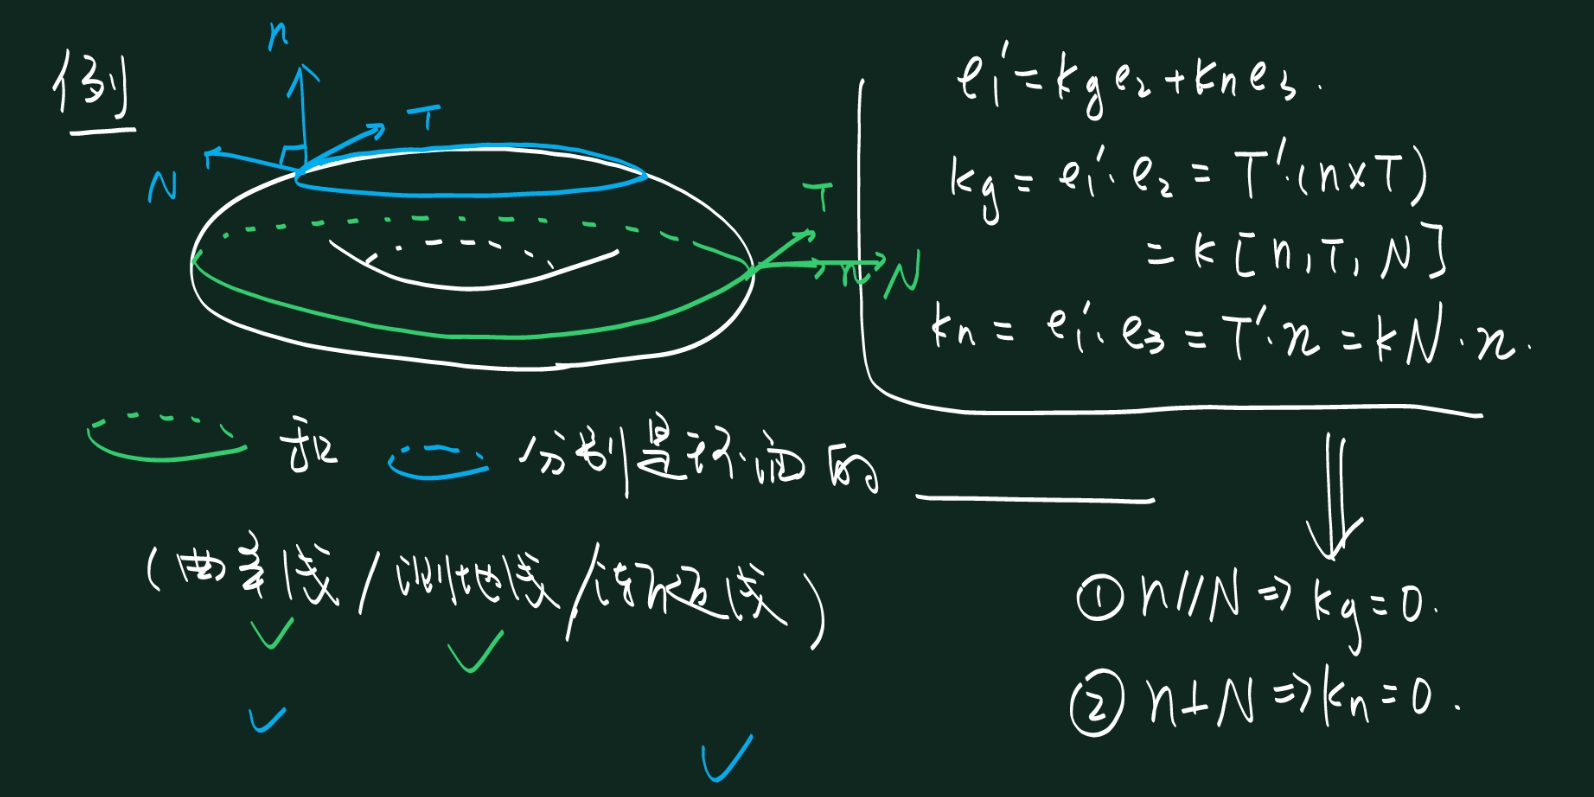
\includegraphics[width=0.8\textwidth]{figure/例题1.png}

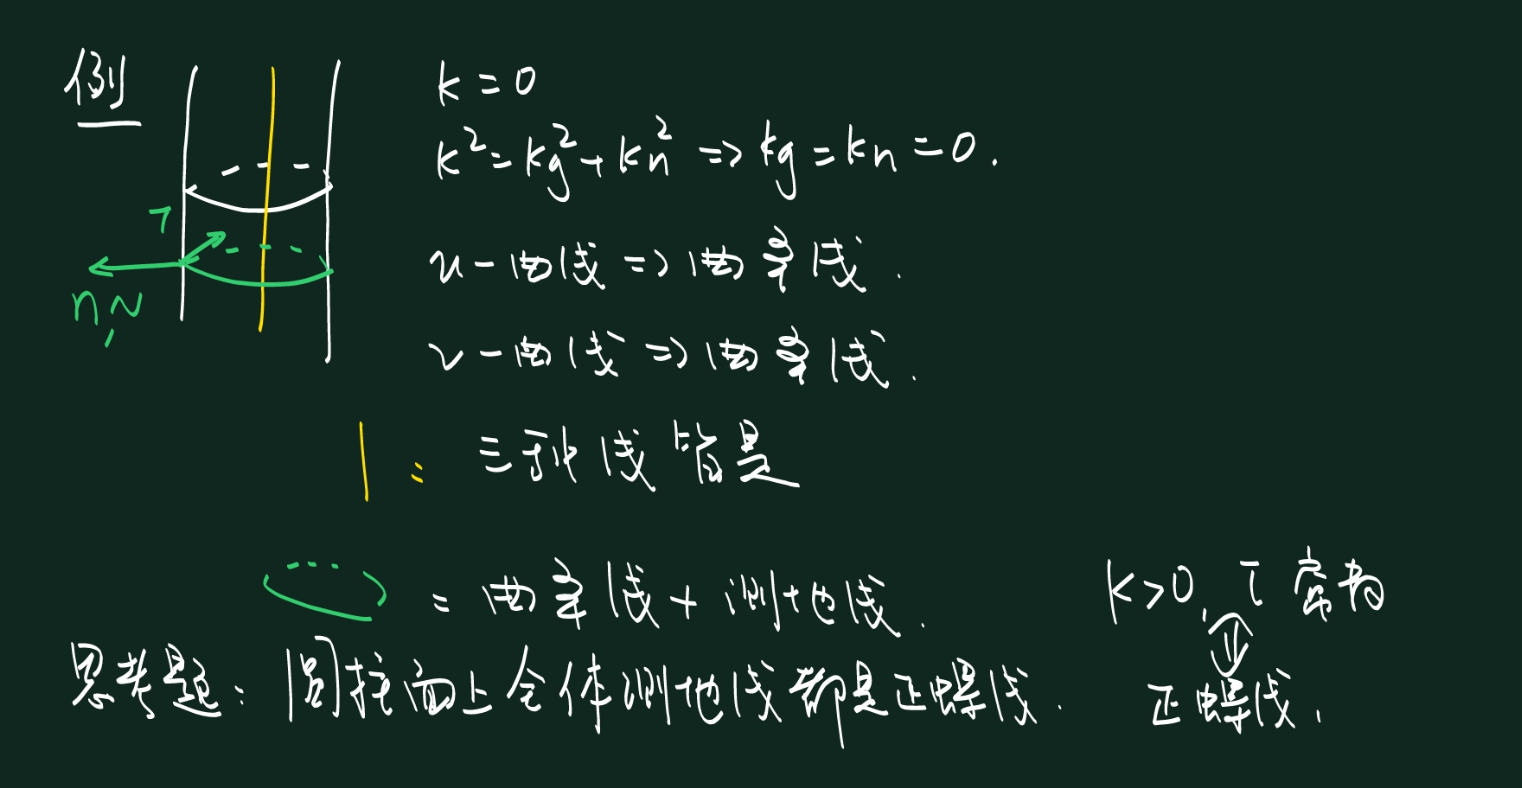
\includegraphics[width=0.8\textwidth]{figure/例题2.png}

\section{测地线的性质}
设 \( r(u^i(s), u^i(s)) \) 为测地线
\[
\Leftrightarrow \frac{d^2 u^k}{ds^2} + \Gamma^k_{ij} \frac{du^i}{ds} \frac{du^j}{ds} = 0.
\]
\begin{theorem}
    \(\forall p \in S, \forall v \in T_pS\),一定存在唯一的测地线
\[
r: (-\epsilon, \epsilon) \rightarrow S, \text{ 满足 } r(0) = p \text{ 且 } r'(0) = v.
\]
\end{theorem}
\begin{proof}
    待定以下函数,\( u^k(s) \) 和 \( v^k(s) \),\( k = 1, 2 \)。

    满足以下 ODE 方程组,
    \[
    \begin{cases}
    \frac{d u^k(s)}{ds} = v^k(s) \\
    \frac{d v^k(s)}{ds} = \Gamma^k_{ij} v^i(s) v^j(s)
    \end{cases}
    \]
    由 ODE 齐次方程组解的存在唯一性定理必然有唯一解,但需要验证 \( r(u^1(s), u^2(s)) \) 确定是以 \( s \) 为弧长参数的测曲线。
目标证明曲线以 \( s \) 为弧长参数,即 \( |r'(s)| = 1 \) 对所有 \( s \) 成立。


切向量表达式:
\[
r'(s) = \frac{\partial r}{\partial u^i} \frac{du^i}{ds} = \frac{dr}{ds}
\]
其模长平方为:
\[
|r'(s)|^2 = r'(s) \cdot r'(s) = g_{ij} \frac{du^i}{ds} \frac{du^j}{ds}
\]
其中 \( g_{ij} = \frac{\partial r}{\partial u^i} \cdot \frac{\partial r}{\partial u^j} \) 是度量张量。\\
定义辅助函数:
\[
h(s) = |r'(s)|^2 - 1 = g_{ij}(u(s)) \frac{du^i}{ds} \frac{du^j}{ds} - 1
\]
由初始条件 \( |r'(0)| = 1 \),有 \( h(0) = 0 \)。若证 \( h(s) \equiv 0 \),则结论成立。


对 \( h(s) \) 求导:
\[
\frac{dh}{ds} = \frac{d}{ds}\left(g_{ij} \frac{du^i}{ds} \frac{du^j}{ds}\right)
\]
展开导数:
\begin{align}
\frac{d}{ds}\left(g_{ij} \frac{du^i}{ds} \frac{du^j}{ds}\right) 
&= \frac{\partial g_{ij}}{\partial u^k} \frac{du^k}{ds} \frac{du^i}{ds} \frac{du^j}{ds} \notag \\
&+ g_{ij} \frac{d^2 u^i}{ds^2} \frac{du^j}{ds} \notag \\
&+ g_{ij} \frac{du^i}{ds} \frac{d^2 u^j}{ds^2} \label{eq:deriv}
\end{align}
利用 \( g_{ij} = g_{ji} \) 的对称性,可合并后两项:
\[
g_{ij} \frac{d^2 u^i}{ds^2} \frac{du^j}{ds} + g_{ij} \frac{du^i}{ds} \frac{d^2 u^j}{ds^2} = 2g_{ij} \frac{d^2 u^i}{ds^2} \frac{du^j}{ds}
\]

由测地线方程:
\[
\frac{d^2 u^i}{ds^2} = -\Gamma_{pq}^i \frac{du^p}{ds} \frac{du^q}{ds}
\]
代入式 (\ref{eq:deriv}) 的第二部分:
\[
2g_{ij} \frac{d^2 u^i}{ds^2} \frac{du^j}{ds} = 2g_{ij}\left( -\Gamma_{pq}^i \frac{du^p}{ds} \frac{du^q}{ds} \right) \frac{du^j}{ds} = -2\Gamma_{pqj} \frac{du^p}{ds} \frac{du^q}{ds} \frac{du^j}{ds}
\]
其中 \( \Gamma_{pqj} = g_{ij}\Gamma_{pq}^i \)。\\
对于第一部分,利用度量张量导数与Christoffel符号的关系:
\[
\frac{\partial g_{ij}}{\partial u^k} = \Gamma_{kij} + \Gamma_{kji}
\]
其中第一类Christoffel符号定义为:
\[
\Gamma_{kij} = \frac{1}{2}\left( \frac{\partial g_{kj}}{\partial u^i} + \frac{\partial g_{ik}}{\partial u^j} - \frac{\partial g_{ij}}{\partial u^k} \right)
\]
代入得:
\[
\frac{\partial g_{ij}}{\partial u^k} \frac{du^k}{ds} \frac{du^i}{ds} \frac{du^j}{ds} = (\Gamma_{kij} + \Gamma_{kji}) \frac{du^k}{ds} \frac{du^i}{ds} \frac{du^j}{ds}
\]

将两部分合并:
\begin{align*}
\frac{dh}{ds} &= (\Gamma_{kij} + \Gamma_{kji}) \frac{du^k}{ds} \frac{du^i}{ds} \frac{du^j}{ds} - 2\Gamma_{pqj} \frac{du^p}{ds} \frac{du^q}{ds} \frac{du^j}{ds} \\
&= \Gamma_{kij} \frac{du^k}{ds} \frac{du^i}{ds} \frac{du^j}{ds} + \Gamma_{kji} \frac{du^k}{ds} \frac{du^i}{ds} \frac{du^j}{ds} - 2\Gamma_{pqj} \frac{du^p}{ds} \frac{du^q}{ds} \frac{du^j}{ds}
\end{align*}
重命名哑指标(\( k \to p \), \( i \to q \), \( j \to j \)):
\[
\frac{dh}{ds} = \Gamma_{pqj} \frac{du^p}{ds} \frac{du^q}{ds} \frac{du^j}{ds} + \Gamma_{pjq} \frac{du^p}{ds} \frac{du^q}{ds} \frac{du^j}{ds} - 2\Gamma_{pqj} \frac{du^p}{ds} \frac{du^q}{ds} \frac{du^j}{ds}
\]
由Christoffel符号的对称性 \( \Gamma_{pjq} = \Gamma_{pqj} \):
\[
\frac{dh}{ds} = \Gamma_{pqj} \frac{du^p}{ds} \frac{du^q}{ds} \frac{du^j}{ds} + \Gamma_{pqj} \frac{du^p}{ds} \frac{du^q}{ds} \frac{du^j}{ds} - 2\Gamma_{pqj} \frac{du^p}{ds} \frac{du^q}{ds} \frac{du^j}{ds} = 0
\]


由 \( \frac{dh}{ds} \equiv 0 \) 和初始条件 \( h(0) = 0 \),根据微分方程解的唯一性,得:
\[
h(s) \equiv 0 \quad \forall s
\]
即:
\[
|r'(s)|^2 = g_{ij} \frac{du^i}{ds} \frac{du^j}{ds} = 1 \quad \Rightarrow \quad |r'(s)| = 1
\]
故曲线 \( r(s) = r(u^1(s), u^2(s)) \) 以 \( s \) 为弧长参数。

\end{proof}
\begin{proposition}
    平面上测地线 \(\Leftrightarrow\) 直线。
\end{proposition}
\begin{proof}
    平面 \( I = (1, 0, 0) \)。
\[
\Rightarrow \Gamma^k_{ij} = 0 \Rightarrow \text{测地线方程 } \frac{d^2 u^k}{ds^2} = 0.
\]
\[
\Rightarrow u^k \text{ 线性} \Rightarrow \text{测地线为直线} 
\]
\end{proof}

事实上,测地线是直线在曲面上的一种推广。

众所周知:平面上两点之间线段最短测地线有类似性质,它的弧长在变分下达到了极值。

下面介绍何为曲线在曲面上的变分
\[
(u^1(s), u^2(s)) \longrightarrow r(u^1(s), u^2(s)),
\]
扰动 \( u^1(s), u^2(s) \) 适当 \(\longrightarrow\) 给出一族曲面上的曲线

\begin{definition}[曲线在曲面上的变分]
    我们称 $\alpha^k: [a, b] \times (-\epsilon, \epsilon) \rightarrow \mathbb{R}^n$,\(k = 1, 2, \ldots\) 为 $u^k: [a, b] \rightarrow \mathbb{R}^n$ 的变分。

    若有 
    \begin{enumerate}
        \item $\alpha^k$ 关于 $t$ 连续,
        \item $\alpha^k(s, 0) = u^k(s)$。
    \end{enumerate}
    
    特别地,我们称其为一个定端变分,若 $\alpha^k(a, t) = u^k(a)$,$\alpha^k(b, t) = u^k(b)$。
    

\end{definition}
在定端变分下,我们也将
\[
r(u^1(s), u^2(s)) \longrightarrow r(s)
\]
\[
r(\alpha^1(s, t), \alpha^2(s, t)) \longrightarrow r_t(s) \text{ 一族头尾固定的曲线。}
\]
我们先记 \( v^k(s) = \left. \frac{d}{dt} \right|_{t=0} \alpha^k(s, t) \),称为变分方向。

\begin{proposition}[弧长变分公式]
\[
\left. \frac{d}{dt} \right|_{t=0} L(r_t) = -\int_a^b g_{ij} v^i \left( \frac{d^2 u^j}{ds^2} + \Gamma^j_{pq} \frac{du^p}{ds} \frac{du^q}{ds} \right) ds.
\]
\end{proposition}




\begin{proof}
    考虑曲线族 \( r_t(s) = r(s,t) \) 满足:
    \begin{itemize}
      \item \( r_0(s) = r(s,0) \) 是参考曲线(以弧长参数化)。
      \item 变分向量场 \( v^i(s) = \left. \frac{\partial u^i}{\partial t} \right|_{t=0} \)。
      \item 固定端点条件:\( v^i(a) = v^i(b) = 0 \)。
    \end{itemize}
    
    长度泛函定义为:
    \[
    L(r_t) = \int_a^b \left| \frac{\partial r}{\partial s} \right| ds = \int_a^b \sqrt{ g_{ij}(u(s,t)) \frac{\partial u^i}{\partial s} \frac{\partial u^j}{\partial s} }  ds.
    \]
    
    在参考曲线 (\( t=0 \)) 上计算变分。由于弧长参数化:
    \[
    \sqrt{ g_{ij} \frac{\partial u^i}{\partial s} \frac{\partial u^j}{\partial s} } \bigg|_{t=0} = 1,
    \]
    因此:
    \begin{align}
        \left. \frac{d}{dt} \right|_{t=0} L(r_t) 
        &= \int_a^b \left. \frac{d}{dt} \right|_{t=0} \sqrt{ g_{ij} \frac{\partial u^i}{\partial s} \frac{\partial u^j}{\partial s} }  ds \nonumber \\
        &= \frac{1}{2} \int_a^b \left. \frac{d}{dt} \right|_{t=0} \left( g_{ij} \frac{\partial u^i}{\partial s} \frac{\partial u^j}{\partial s} \right) ds \label{eq:main} \\
        &= \frac{1}{2} \int_a^b \left[ \left( \partial_k g_{ij} v^k \right) \frac{du^i}{ds} \frac{du^j}{ds} + 2g_{ij} \frac{du^j}{ds} \frac{\partial v^i}{\partial s} \right] ds, \nonumber
    \end{align}
    其中 \( \frac{du^i}{ds} = \left. \frac{\partial u^i}{\partial s} \right|_{t=0} \) 是参考曲线的切向量。
    
    对含 \( \frac{\partial v^i}{\partial s} \) 的项进行分部积分:
    \[
    \int_a^b g_{ij} \frac{du^j}{ds} \frac{\partial v^i}{\partial s}  ds = \left[ g_{ij} \frac{du^j}{ds} v^i \right]_a^b - \int_a^b \frac{\partial}{\partial s} \left( g_{ij} \frac{du^j}{ds} \right) v^i  ds.
    \]
    由固定端点条件 \( v^i(a) = v^i(b) = 0 \),边界项为零:
    \[
    \int_a^b g_{ij} \frac{du^j}{ds} \frac{\partial v^i}{\partial s}  ds = - \int_a^b \left( \partial_k g_{ij} \frac{du^k}{ds} \frac{du^j}{ds} + g_{ij} \frac{d^2 u^j}{ds^2} \right) v^i  ds. \label{eq:partial_int}
    \]
    
    将式 \eqref{eq:partial_int} 代入式 \eqref{eq:main}:
    \begin{align}
        \left. \frac{d}{dt} \right|_{t=0} L(r_t) 
        &= \frac{1}{2} \int_a^b \left[ \partial_k g_{ij} v^k \frac{du^i}{ds} \frac{du^j}{ds} - 2 \left( \partial_k g_{ij} \frac{du^k}{ds} \frac{du^j}{ds} + g_{ij} \frac{d^2 u^j}{ds^2} \right) v^i \right] ds \nonumber \\
        &= \frac{1}{2} \int_a^b v^i \left[ \partial_i g_{jk} \frac{du^j}{ds} \frac{du^k}{ds} - 2 \partial_j g_{ik} \frac{du^j}{ds} \frac{du^k}{ds} - 2 g_{ij} \frac{d^2 u^j}{ds^2} \right] ds. \label{eq:combined}
    \end{align}
    
    由 Christoffel 符号的定义(第一类):
    \[
    \Gamma_{ijk} = \frac{1}{2} \left( \partial_j g_{ik} + \partial_k g_{ij} - \partial_i g_{jk} \right),
    \]
    则式 \eqref{eq:combined} 中导数项的系数可表示为:
    \begin{align*}
        \partial_i g_{jk} - 2 \partial_j g_{ik} 
        &= \left[ -2 \Gamma_{ijk} + (\partial_j g_{ik} + \partial_k g_{ij} - \partial_i g_{jk}) \right] - 2 \partial_j g_{ik} \\
        &= -2 \Gamma_{ijk} - \partial_j g_{ik} + \partial_k g_{ij}.
    \end{align*}
    代入式 \eqref{eq:combined}:
    \begin{align*}
        \left. \frac{d}{dt} \right|_{t=0} L(r_t) 
        &= \frac{1}{2} \int_a^b v^i \left[ \left( -2 \Gamma_{ijk} - \partial_j g_{ik} + \partial_k g_{ij} \right) \frac{du^j}{ds} \frac{du^k}{ds} - 2 g_{ij} \frac{d^2 u^j}{ds^2} \right] ds \\
        &= \frac{1}{2} \int_a^b v^i \left[ -2 \Gamma_{ijk} \frac{du^j}{ds} \frac{du^k}{ds} - (\partial_j g_{ik} - \partial_k g_{ij}) \frac{du^j}{ds} \frac{du^k}{ds} - 2 g_{ij} \frac{d^2 u^j}{ds^2} \right] ds.
    \end{align*}
    由于 \( \partial_j g_{ik} - \partial_k g_{ij} \) 关于指标 \( j,k \) 反对称,而 \( \frac{du^j}{ds} \frac{du^k}{ds} \) 对称,其乘积为零:
    \[
    (\partial_j g_{ik} - \partial_k g_{ij}) \frac{du^j}{ds} \frac{du^k}{ds} = 0.
    \]
    因此:
    \[
    \left. \frac{d}{dt} \right|_{t=0} L(r_t) = \frac{1}{2} \int_a^b v^i \left[ -2 \Gamma_{ijk} \frac{du^j}{ds} \frac{du^k}{ds} - 2 g_{ij} \frac{d^2 u^j}{ds^2} \right] ds.
    \]
    
    将第一类 Christoffel 符号转换为第二类 \( \Gamma_{jk}^l = g^{lm} \Gamma_{jkm} \),并利用 \( \Gamma_{ijk} = g_{il} \Gamma_{jk}^l \):
    \begin{align*}
        \left. \frac{d}{dt} \right|_{t=0} L(r_t) 
        &= -\int_a^b v^i \left[ g_{il} \Gamma_{jk}^l \frac{du^j}{ds} \frac{du^k}{ds} + g_{il} \frac{d^2 u^l}{ds^2} \right] ds \\
        &= -\int_a^b g_{il} v^i \left( \frac{d^2 u^l}{ds^2} + \Gamma_{jk}^l \frac{du^j}{ds} \frac{du^k}{ds} \right) ds.
    \end{align*}
    重新标记哑指标 \( l \to j \),即得:
    \[
    \left. \frac{d}{dt} \right|_{t=0} L(r_t) = -\int_a^b g_{ij} v^i \left( \frac{d^2 u^j}{ds^2} + \Gamma^j_{pq} \frac{du^p}{ds} \frac{du^q}{ds} \right) ds.
    \]
    
    当参考曲线是测地线时,满足测地线方程:
    \[
    \frac{d^2 u^j}{ds^2} + \Gamma^j_{pq} \frac{du^p}{ds} \frac{du^q}{ds} = 0,
    \]
    因此:
    \[
    \left. \frac{d}{dt} \right|_{t=0} L(r_t) = 0,
    \]
    这表明测地线是长度泛函的临界点。
\end{proof}
\begin{corollary}
    若曲线为测地线 \(\Rightarrow \left. \frac{d}{dt} \right|_{t=0} L(r_t) = 0\)。
\end{corollary}

\begin{theorem}
    \( r(s) \) 是变分中的弧长达到极值的曲线 \(\Leftrightarrow r(s)\) 为测地线。
\end{theorem}
\begin{proof}
    \textbf{(\(\Leftarrow\))方向:} 若 \( r(s) \) 为测地线,则测地曲率 \( k_g = 0 \)。由变分法基本公式,弧长一阶变分为:
    \[
    \left. \frac{d}{dt} \right|_{t=0} L(r_t) = 0
    \]
    因此弧长达到临界值(极值条件)。
    
    \textbf{(\(\Rightarrow\))方向:} 若对任意变分 \( v_t \) 满足端点固定(即 \( v^k(a) = v^k(b) = 0 \)),都有:
    \[
    \left. \frac{d}{dt} \right|_{t=0} L(v_t) = 0
    \]
    构造特殊变分场:
    \[
    v^k(s) = \sin \left( \frac{\pi (s - a)}{b - a} \right) \left[ \frac{d^2 u^k}{ds^2} + \Gamma_{ij}^k \frac{du^i}{ds} \frac{du^j}{ds} \right]
    \]
    其中 \( u^k \) 是 \( r(s) \) 的局部坐标表示。易验证:
    \[
    v^k(a) = \sin(0) \cdot [\cdots] = 0, \quad v^k(b) = \sin(\pi) \cdot [\cdots] = 0
    \]
    满足端点条件。代入一阶变分公式得:
    \[
    0 = -\int_a^b \sin \left( \frac{\pi (s - a)}{b - a} \right) \cdot k_g^2  \dd s
    \]
    其中 \( k_g^2 = g_{kl} \left( \frac{d^2 u^k}{ds^2} + \Gamma_{ij}^k \frac{du^i}{ds} \frac{du^j}{ds} \right) \left( \frac{d^2 u^l}{ds^2} + \Gamma_{mn}^l \frac{du^m}{ds} \frac{du^n}{ds} \right) \) 是测地曲率平方。
    
    由于度量正定,\( k_g^2 \geq 0 \) 恒成立,且被积函数中:
    \[
    \sin \left( \frac{\pi (s - a)}{b - a} \right) > 0, \quad \forall s \in (a,b)
    \]
    因此有:
    \[
    \int_a^b \underbrace{\sin \left( \frac{\pi (s - a)}{b - a} \right)}_{>0} \cdot \underbrace{k_g^2}_{\geq 0}  \dd s = 0
    \]
    这要求 \( k_g^2 = 0 \) 在 \([a,b]\) 上几乎处处成立。由连续性,\( k_g(s) = 0 \) 对所有 \( s \in [a,b] \) 成立,故 \( r(s) \) 是测地线。
    
   
    \[
    k_g e_2 = \left( \frac{d^2 u^k}{ds^2} + \Gamma_{ij}^k \frac{du^i}{ds} \frac{du^j}{ds} \right) \vec{e}_k
    \]
    当 \( k_g = 0 \) 时,测地方程成立。
\end{proof}

\section{参数网}
事实上曲面每点处局部可选择特殊的参考。
(u, v) 使得在局部上计算变得简洁。
这件事情需要基于以下引理。

\begin{lemma}
    设 $f, g \in C^1(D)$,$D \subset \mathbb{R}^2$,$\forall p \in D$,在 $U \subset D$ 使得总存在 $F \in C^1(D)$ 和 $\lambda \in C(U)$,使
\[
dF = \lambda (f \, du + g \, dv).
\]
\end{lemma}

\begin{lemma}
    设 $r: D \rightarrow \mathbb{R}^3$ 为正则曲面,\(a(u,v)\) 和 \(b(u,v)\) 是 \(D\) 上的两个向量场(切向量的分布)。

(即 \(\forall (u_0,v_0) \in D\),\(a(u_0,v_0) \in T_{(u_0,v_0)}S\)。)
那么 \(\forall p \in D\),总是存在 \(p \in U \subseteq D\) 使得在 \(U\) 上可取到新参数 \((\widetilde{u}, \widetilde{v})\) 

满足 \(r_{\widetilde{u}} \parallel a\),\(r_{\widetilde{v}} \parallel b\),\(\forall (u,v) \in U\)。
\end{lemma}

\begin{proof}
    在每点 \( T_{(u,v)}S \) 上,总有 \( a_1(u,v) \) 和 \( a_2(u,v) \) 正交,
\[
\text{使 } a(u,v) = a_1(u,v) r_u(u,v) + a_2(u,v) r_v(u,v).
\]
以下简记为
\[
a = a_1 r_u + a_2 r_v.
\]
同理有
\[
b = b_1 r_u + b_2 r_v.
\]
定义矩阵 \( A = \begin{bmatrix} a_1 & a_2 \\ b_1 & b_2 \end{bmatrix} \),则 \( a, b \) 线性无关当且仅当
\[
\det A = a_1 b_2 - a_2 b_1 \neq 0, \quad \forall (u,v) \in D.
\]

由引理可知,\(\forall p \in D\),一定存在邻域 \( p \in U \subseteq D \),在 \( U \) 上有 \(\widetilde{u}, \widetilde{v} \in C^1(U)\) 和函数 \(\lambda, \mu \in C(U)\),使得
\[
\begin{cases}
d\widetilde{u} = \lambda (b_2 du - b_1 dv) \\
d\widetilde{v} = \mu (-a_2 du + a_1 dv)
\end{cases}
\]
并满足
\[
r_{\widetilde{u}} \parallel a, \quad r_{\widetilde{v}} \parallel b.
\]

容易看出,坐标变换的 Jacobi 矩阵为
\[
\frac{\partial (\widetilde{u}, \widetilde{v})}{\partial (u,v)} = \begin{bmatrix} \widetilde{u}_u & \widetilde{u}_v \\ \widetilde{v}_u & \widetilde{v}_v \end{bmatrix} = \begin{bmatrix} \lambda b_2 & -\lambda b_1 \\ -\mu a_2 & \mu a_1 \end{bmatrix}.
\]
其逆矩阵为
\[
\frac{\partial (u,v)}{\partial (\widetilde{u}, \widetilde{v})} = \frac{1}{\lambda \mu \det A} \begin{bmatrix} \mu a_1 & \lambda b_1 \\ \mu a_2 & \lambda b_2 \end{bmatrix}.
\]
于是
\[
r_{\widetilde{u}} = \frac{\partial u}{\partial \widetilde{u}} r_u + \frac{\partial v}{\partial \widetilde{u}} r_v = \frac{1}{\lambda \det A} (a_1 r_u + a_2 r_v) = \frac{1}{\lambda \det A} a \implies r_{\widetilde{u}} \parallel a.
\]
同理,
\[
r_{\widetilde{v}} = \frac{\partial u}{\partial \widetilde{v}} r_u + \frac{\partial v}{\partial \widetilde{v}} r_v = \frac{1}{\mu \det A} (b_1 r_u + b_2 r_v) = \frac{1}{\mu \det A} b \implies r_{\widetilde{v}} \parallel b.
\]
\end{proof}
\subsection{正交参数网(局部上F=0)}
对于任意的 $(u,v)$ 参数,作 Schmit 正交化。

令 $e_1 = \frac{r_u}{\sqrt{E}}$ 单位向量。

令 $b = r_v - \lambda e_1$,要求 $b \cdot e_1 = 0$,算 $\lambda$。
\[
\Rightarrow (r_v - \lambda e_1) \cdot e_1 = 0 \Rightarrow \lambda = r_v \cdot e_1 = r_v \cdot \frac{r_u}{\sqrt{E}} = \frac{F}{\sqrt{E}}.
\]
\[
\Rightarrow b = r_v - \frac{F}{E} r_u.
\]
\[
b \cdot b = G - \frac{2E^2}{E} + \frac{F^2}{E} = G - \frac{F^2}{E} = \frac{EG - F^2}{E}.
\]

令 $e_2 = \frac{b}{|b|} = \frac{r_v - \frac{F}{E} r_u}{\sqrt{EG - F^2 / E}}$。

$\{e_1, e_2\}$ 单位正交向量场。

由引理可知,局部上总有 $(\widetilde{u}, \widetilde{v})$ 正交参数,
\[
\text{使 } r_{\widetilde{u}} \parallel e_1, \quad r_{\widetilde{v}} \parallel e_2.
\]
\[
\Rightarrow \text{在 } (\widetilde{u}, \widetilde{v}) \text{ 坐标下 } F \text{ 局部恒为 } 0.
\]
我们称这样的 $(\widetilde{u}, \widetilde{v})$ 是正交网。
\subsection{曲率线参数网(局部上 \(F = M = 0\))}
假设 $P$ 是 $S$ 上的非脐点(脐点 $k_1 = k_2$)。

那么我们可取 $k_1$ 和 $k_2$ 对应的特征方向 $v_1, v_2$。

$(k_1, k_2$ 是 $C^1$ 的。$\left\{
\begin{array}{l}
k = k_1 \cdot k_2 \\
H = \frac{k_1 + k_2}{2}
\end{array}
\right. \Rightarrow v_1, v_2$ 是两个 $C'$、线性无关向量场)

自然局部上可取到 $(\widetilde{u}, \widetilde{v})$ 使得 $r_{\widetilde{u}} \parallel v_1$,$r_{\widetilde{v}} \parallel v_2$。

注意到 $v_1 \perp v_2$(两个特征值的特征方向)。

$\Rightarrow \widetilde{F} = 0$。取 $\omega$ 为 Weingarten 算子。

\[
\Rightarrow
\left\{
\begin{array}{l}
\omega(r_{\widetilde{u}}) = -n_{\widetilde{u}} = k_1 r_{\widetilde{u}} \cdot \\
\omega(r_{\widetilde{v}}) = -n_{\widetilde{v}} = k_2 r_{\widetilde{v}}
\end{array}
\right.
\left(
\begin{array}{l}
\omega(v_1) = k_1 v_1 \\
\omega(v_2) = k_2 v_2
\end{array}
\right)
\]

\[
\Rightarrow
\left\{
\begin{array}{l}
\widetilde{L} = -n_{\widetilde{u}} \cdot r_{\widetilde{u}} = k_1 r_{\widetilde{u}} \cdot r_{\widetilde{u}} = k_1 \widetilde{E} \\
\widetilde{M} = -n_{\widetilde{u}} \cdot r_{\widetilde{v}} = k_1 r_{\widetilde{u}} \cdot r_{\widetilde{v}} = 0 \\
\widetilde{N} = -n_{\widetilde{v}} \cdot r_{\widetilde{v}} = k_2 r_{\widetilde{v}} \cdot r_{\widetilde{v}} = k_2 \widetilde{G}
\end{array}
\right.
\]

若用曲率线网,则局部上
\[
I= E \, du \otimes du + G \, dv \otimes dv
\]
而
\[
II = k_1 E \, du \otimes du + k_2 G \, dv \otimes dv.
\]

\begin{example}
    设 $S$ 为已测曲面,$P$ 为其上的非脐点。

    \begin{enumerate}
        \item 设 $r(s)$ 过 $P$ 以 $S$ 为弧长的一条曲面上曲线,$\theta$ 为对应的切向角,则有以下公式:
        \[
        \tau_g = (k_2 - k_1) \sin \theta \cos \theta.
        \]

        \item 证明:若过 $P$ 可作两条渐近线,则
        \[
        \tau_{g_1} = -\tau_{g_2}.
        \]

        \item 证明:$\tau_{g_1} \cdot \tau_{g_2} = K_p$。(CMC原题)
    \end{enumerate}

\end{example}
\begin{proof}
    (1)给定第一基本形式和第二基本形式:
    \[
    I = E  du^2 + 2F  du  dv + G  dv^2, \quad II = L  du^2 + 2M  du  dv + N  dv^2
    \]
    曲线切向量表示为:
    \[
    r'(s) = \frac{du}{ds} \mathbf{r}_u + \frac{dv}{ds} \mathbf{r}_v = \left( \frac{du}{ds} \sqrt{E} \right) \frac{\mathbf{r}_u}{\sqrt{E}} + \left( \frac{dv}{ds} \sqrt{G} \right) \frac{\mathbf{r}_v}{\sqrt{G}}
    \]
    其中单位切向分量满足:
    \[
    \frac{du}{ds} \sqrt{E} = \cos \theta, \quad \frac{dv}{ds} \sqrt{G} = \sin \theta
    \]
    即:
    \[
    \frac{du}{ds} = \frac{\cos \theta}{\sqrt{E}}, \quad \frac{dv}{ds} = \frac{\sin \theta}{\sqrt{G}}
    \]
    \[
    \tau_g = (k_2 - k_1) \sin \theta \cos \theta
    \]

    (2)由 Euler 公式:
    \[
    k_n = k_1 \cos^2 \theta + k_2 \sin^2 \theta = 0
    \]
    解得:
    \[
    \tan^2 \theta = -\frac{k_1}{k_2} \quad (\text{要求 } k_1 k_2 < 0 \text{,即 } P \text{ 为双曲点})
    \]
    对两条曲线,有 \( \tan^2 \theta_1 = \tan^2 \theta_2 \),故:
    \[
    \theta_1 = -\theta_2 \quad (\text{方向相反})
    \]
    由测地曲率公式:
    \[
    \tau_{g1} = (k_2 - k_1) \sin \theta_1 \cos \theta_1, \quad \tau_{g2} = (k_2 - k_1) \sin(-\theta_1) \cos(-\theta_1) = -(k_2 - k_1) \sin \theta_1 \cos \theta_1
    \]
    因此:
    \[
    \tau_{g1} = -\tau_{g2}
    \]

    (3)由 (2) 知 \( T_{g2} = -T_{g1} \),且两条曲线均为渐近曲线(\( k_n = 0 \))。  
    计算乘积:
    \[
    \tau_{g1} \tau_{g2} = \tau_{g1} (-\tau_{g1}) = -\tau_{g1}^2 = - \left[ (k_2 - k_1) \sin \theta_1 \cos \theta_1 \right]^2 = - (k_2 - k_1)^2 \sin^2 \theta_1 \cos^2 \theta_1
    \]
    由 Euler 公式 \( k_n = 0 \) 导出关系:
    \begin{align*}
    k_1 \cos^2 \theta_1 + k_2 \sin^2 \theta_1 &= 0 \\
    \Rightarrow k_1 &= -(k_2 - k_1) \sin^2 \theta_1 \\
    k_2 &= (k_2 - k_1) \cos^2 \theta_1
    \end{align*}
    代入乘积式:
    \[
    - (k_2 - k_1)^2 \sin^2 \theta_1 \cos^2 \theta_1 = - \left[ (k_2 - k_1) \sin^2 \theta_1 \right] \left[ (k_2 - k_1) \cos^2 \theta_1 \right] = - \left[ -k_1 \right] \left[ k_2 \right] = k_1 k_2
    \]
    高斯曲率 \( K_p = k_1 k_2 \),故:
    \[
    \tau_{g1} \tau_{g2} = K_p
    \]
\end{proof}
\begin{example}
    $\mathbf{III} = dn \cdot dn$ 满足恒等式。
\[
\mathbf{III} - 2H\mathbf{II} + k\mathbf{I} = 0.
\]
\end{example}
\begin{proof}
    公式可逐项证明,故而可逐项取曲率线网。
\[
\mathbf{I} = E \, du \otimes du + G \, dv \otimes dv
\]
\[
\mathbf{II} = k_1 E \, du \otimes du + k_2 G \, dv \otimes dv
\]
\[
\mathbf{III} = k_1^2 E \, du \otimes du + k_2^2 G \, dv \otimes dv.
\]
\[
e = n_u \cdot n_u = k_1^2 E, \quad f = 0, \quad g = k_2^2 G \, dv \otimes dv.
\]
    直接验证即可
\end{proof}


\begin{theorem}
    平面上两点之间可微曲线之中线段最短。
\end{theorem}
\begin{proof}
    设 $P, Q \in \Sigma$,以 $P$ 为原点建立极坐标系 $(\rho, \theta)$。

\[
r(x, y) = (x, y, 0) = (\rho \cos \theta, \rho \sin \theta, 0).
\]
\[
r_{\rho} = (\cos \theta, \sin \theta, 0), \quad r_{\theta} = (-\rho \sin \theta, \rho \cos \theta, 0).
\]
\[
E = 1, \quad F = 0, \quad G = \rho^2.
\]
\[
I = d\rho \otimes d\rho + \rho^2 d\theta \otimes d\theta.
\]

设 $r: [0,1] \rightarrow \Sigma$ 为连接 $P, Q$ 的任意曲线。
\[
r(0) = P, \quad r(1) = Q, \quad r'(t) = \frac{d\rho}{dt} r_{\rho} + \frac{d\theta}{dt} r_{\theta}.
\]
\[
L(\widehat{PQ}) = \int_0^1 \left| \frac{dr}{dt} \right| dt = \int_0^1 \sqrt{\left( \frac{d\rho}{dt} \right)^2 + \rho^2 \left( \frac{d\theta}{dt} \right)^2} dt.
\]
\[
\geq \int_0^1 \frac{d\rho}{dt} dt = (\rho(1) - \rho(0)).\text{P 到 Q 的距离}.
\]
\[
\text{等号成立当且仅当 } \frac{d\theta}{dt} = 0 \Rightarrow \theta \text{ 常数} \Rightarrow \text{线段}.
\]

\end{proof}
我们希望仿照平面的极坐标给出曲面上的“极坐标系”。
\begin{definition}[指数映射]
    $\forall p \in S$.
\[
\exp_p: T_pS \longrightarrow S.
\]
\[
\sim \longmapsto r_v(1).
\]
我们之前证明过,$\forall p \in S$,$\forall v \in T_pM$,局部上总有测地线 $r_v(t)$ 满足 $r_v(0) = p$,$r_v'(0) = v$。
\end{definition}
\begin{lemma}\label{lemma}
    \( r_v(s) = r_{\frac{v}{\rho}}(\rho s) \), \(\forall \rho > 0 \in \mathbb{R}\).
\end{lemma}
\begin{proof}
    曲线形状一致,且
    \begin{enumerate}
        \item \(\displaystyle r_{\frac{v}{\rho}}(0) = \rho\).
        \item \(\displaystyle r'_{\frac{v}{\rho}}(0) = \rho \cdot \frac{v}{\rho} = v\).
    \end{enumerate}
    
    \textbf{由唯一性可知}
    \[
    r_v(s) = r_{\frac{v}{\rho}}(\rho s)
    \]
\end{proof}

\textbf{FACT} \quad \( r_v(s) = \exp_{\rho}(sv) \).
\begin{proof}
    \(\exp_{\rho}(sv) = r_{sv}(1)\) 引理\ref{lemma} \(r_v(s)\) \(\downarrow\)
\end{proof}


\textbf{FACT} \(\left. \frac{d}{ds} \right|_{s=0} \exp_{\rho}(sv) = \left. \frac{d}{ds} \right|_{s=0} r_v(s) = r'_v(0) = v\).





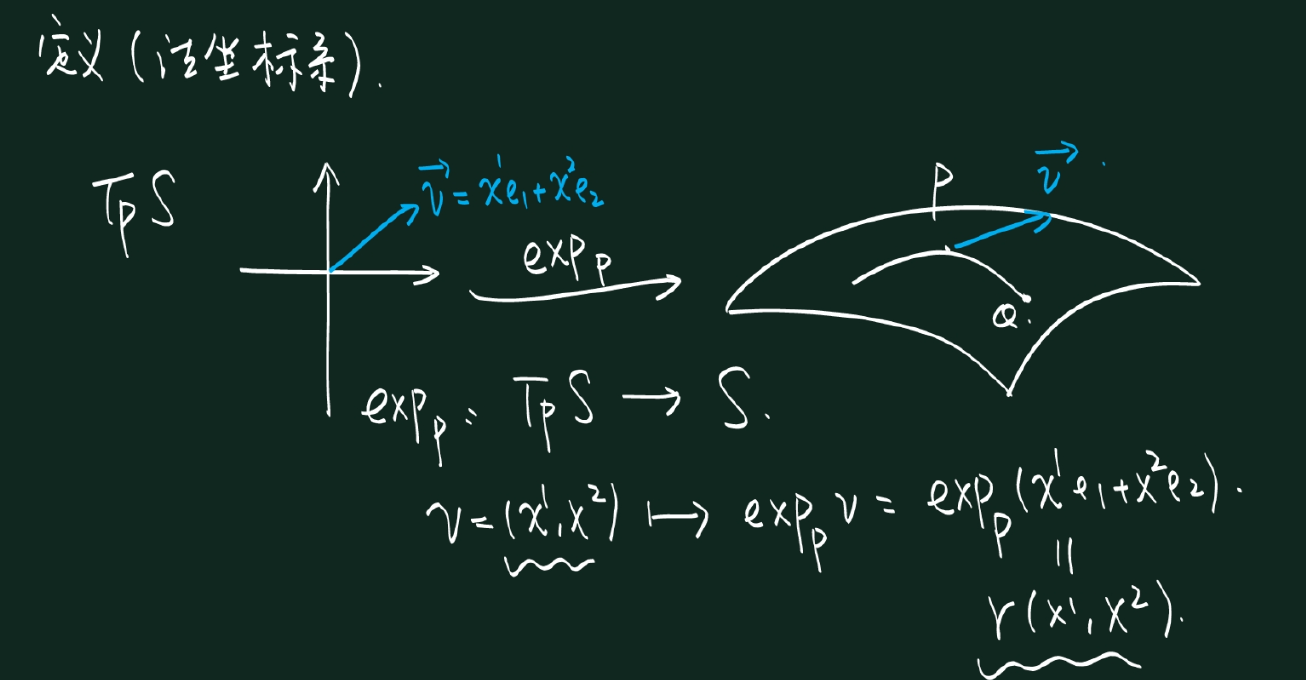
\includegraphics[width=0.8\textwidth]{figure/法坐标系.png}

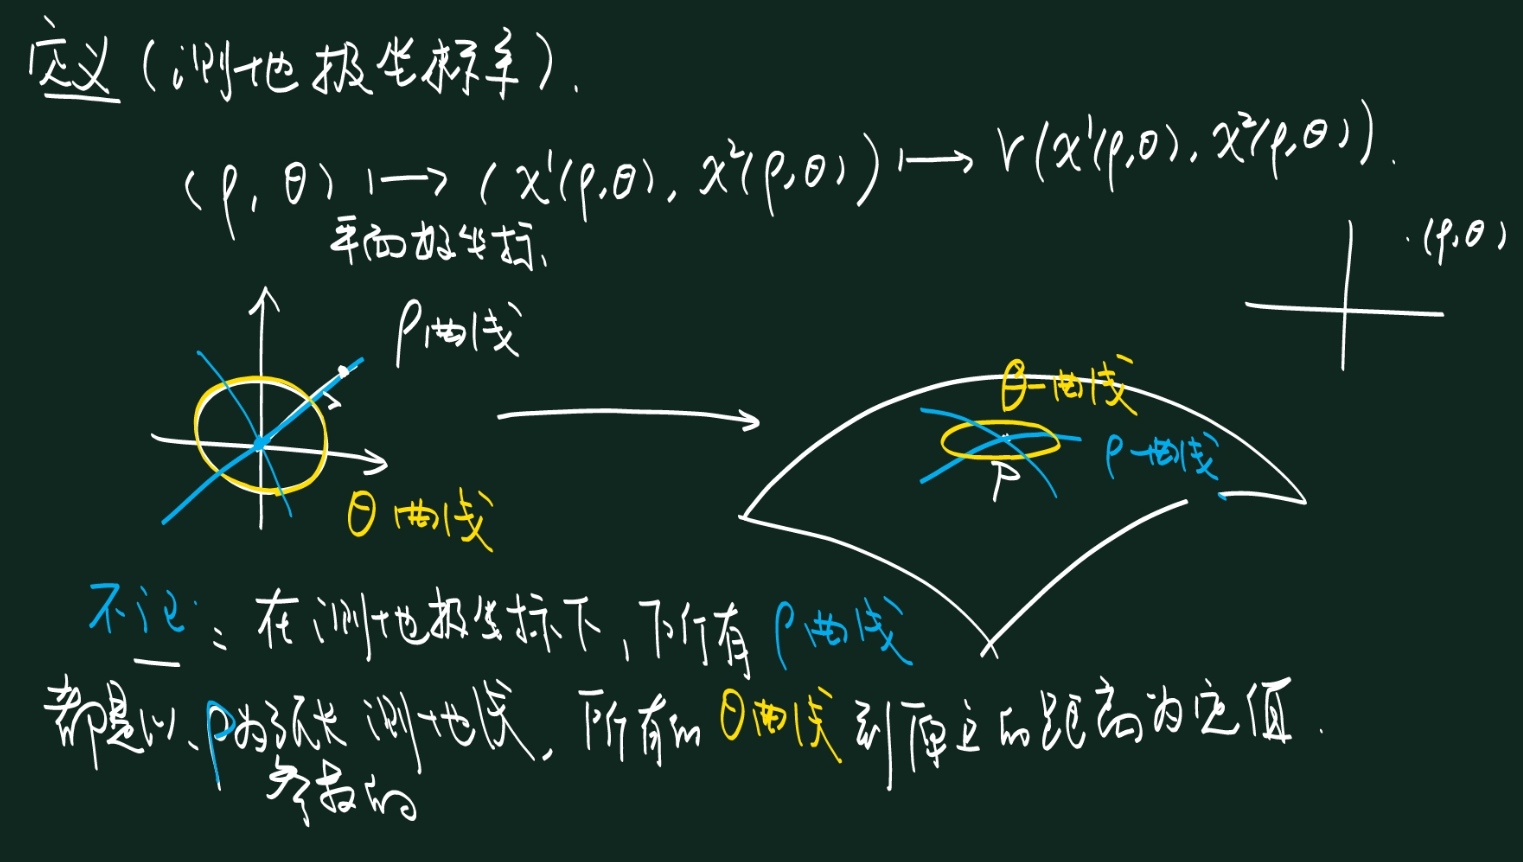
\includegraphics[width=0.8\textwidth]{figure/测地坐标系.png}


这个没图不行,直接给图了


\begin{lemma}[Gauss 引理]
    在曲面测地极坐标系中,\(\forall P\) 曲线都彼此正交。
\end{lemma}
\begin{proof}
    设曲面参数化为 \( r(\rho, \theta) \),其中:
\begin{align*}
r_\rho &= \frac{\partial r}{\partial \rho} = r_1 \cos \theta + r_2 \sin \theta \\
r_\theta &= \frac{\partial r}{\partial \theta} = \rho (-r_1 \sin \theta + r_2 \cos \theta)
\end{align*}
其中 \( r_1 = \frac{\partial r}{\partial u^1} \), \( r_2 = \frac{\partial r}{\partial u^2} \) 是坐标基向量。

\begin{enumerate}
    \item \begin{align*}
        F(\rho, \theta) &= r_\rho \cdot r_\theta \\
        &= (r_1 \cos \theta + r_2 \sin \theta) \cdot \rho (-r_1 \sin \theta + r_2 \cos \theta) \\
        &= \rho \left[ \cdots \right] \quad \text{(点积展开)}
        \end{align*}
        当 \(\rho \to 0\) 时(即趋向极点),有:
        \[
        \lim_{\rho \to 0} F(\rho, \theta) = 0.
        \]
    
    \item 计算 \( F \) 对 \(\rho\) 的偏导数:
    \begin{align*}
    \frac{\partial F}{\partial \rho} &= \frac{\partial}{\partial \rho} (r_\rho \cdot r_\theta) \\
    &= r_{\rho\rho} \cdot r_\theta + r_\rho \cdot r_{\rho\theta}
    \end{align*}
    其中 \( r_{\rho\rho} = \frac{\partial^2 r}{\partial \rho^2} \), \( r_{\rho\theta} = \frac{\partial^2 r}{\partial \rho \partial \theta} \).
    
    由曲面理论,二阶导数可用 Christoffel 符号表示:
    \[
    r_{\rho\rho} = \Gamma_{11}^1 r_\rho + \Gamma_{11}^2 r_\theta
    \]
    但关键性质是:\(\rho\)-曲线是测地线,且以 \(\rho\) 为弧长参数。测地线方程给出:
    \[
    \frac{d^2 u^k}{d\rho^2} + \Gamma_{ij}^k \frac{du^i}{d\rho} \frac{du^j}{d\rho} = 0
    \]
    对于 \(\rho\)-曲线(固定 \(\theta\)),有 \( du^1/d\rho = \cos \theta \), \( du^2/d\rho = \sin \theta \),且 \( d^2 u^k/d\rho^2 = 0 \)。代入得:
    \[
    \Gamma_{11}^k \cos^2 \theta + 2\Gamma_{12}^k \cos\theta \sin\theta + \Gamma_{22}^k \sin^2 \theta = 0
    \]
    特别地,当坐标系在极点正则时,有 \(\Gamma_{11}^k = 0\).
    
    同时,由弧长参数化条件:
    \[
    |r_\rho|^2 = 1 \implies \frac{\partial}{\partial \theta} (|r_\rho|^2) = 2 r_\rho \cdot r_{\rho\theta} = 0
    \]
    因此:
    \[
    \frac{\partial F}{\partial \rho} = (\Gamma_{11}^1 r_\rho + \Gamma_{11}^2 r_\theta) \cdot r_\theta + \frac{1}{2} \frac{\partial}{\partial \theta} (|r_\rho|^2) = 0
    \]
    故 \( F \) 与 \(\rho\) 无关,为常数。
\end{enumerate}

由边界条件:
\[
\lim_{\rho \to 0} F(\rho, \theta) = 0
\]
且 \( F \) 是常数,故对任意 \(\rho > 0\),
\[
F(\rho, \theta) = r_\rho \cdot r_\theta = 0
\]
正交性得证。
\end{proof}
\begin{proposition}
    法坐标系满足以下性质:
\begin{enumerate}
    \item \( g_{ij}(0,0) = \delta_{ij} \) \quad (即 \( P \) 点处的第一基本形式为 \( E_2 \))
    \item \( \Gamma^k_{ij}(0,0) = 0, \quad \forall i,j,k \).
\end{enumerate}
\end{proposition}
\begin{proof}
    \begin{enumerate}
        \item \( r(x^1, x^2) = \exp_{\rho}(x^1 e_1 + x^2 e_2) \)
        \[
        \left. \frac{\partial r}{\partial x^i} \right|_{(0,0)} = \left. \frac{d}{dx^i} \right|_{x^i=0} \exp_{\rho}(x^1 e_1) = \left. \frac{d}{dt} \right|_{t=0} \exp_{\rho}(t e_i) = e_i
        \]
        同理 \(\left. \frac{\partial r}{\partial x^2} \right|_{(0,0)} = e_2\),由 \(e_1, e_2\) 单位正交 \(\Rightarrow g_{ij}(0,0) = \delta_{ij}\)。
        \item 注意在测地极坐标系下,\(r(\rho, \theta)\) 的 \(\rho\)-曲线为测地线:$ \left\{
            \begin{array}{l}
            x^1 = \rho \cos \theta \\
            x^2 = \rho \sin \theta
            \end{array}
            \right.$
        \[
        \text{测地线方程:} \quad \frac{d^2 x^k}{d\rho^2} + \Gamma^k_{ij} \frac{dx^i}{d\rho} \frac{dx^j}{d\rho} = 0.
        \]
        \[
        r(x^1(\rho), x^2(\rho)) \quad \Rightarrow \quad \Gamma^k_{ij} f(\theta) = 0, \quad \forall \theta \quad \Rightarrow \quad \Gamma^k_{ij} = 0.
        \]
       
    \end{enumerate}
    
\end{proof}
\begin{proposition}
    测地极坐标一定满足以下性质。

\begin{enumerate}
    \item $I = d\rho \otimes d\rho + G(\rho, \theta) d\theta \otimes d\theta.$ ($E = 1, F = 0$).(Gauss 引理)
    \item $\lim_{\rho \to 0} \sqrt{G} = 0.$ (对照欧氏公式 $G = \rho^2$).
    \item $\lim_{\rho \to 0} \frac{\partial}{\partial \rho} \sqrt{G} = 1.$
    \item $K = \frac{-(\sqrt{G})_{\rho\rho}}{\sqrt{G}}$
\end{enumerate}
\end{proposition}
\begin{proof}
    \begin{enumerate}
        \item \begin{itemize}
            \item \( E = 1 \):因为 \(\rho\) 是径向测地线的弧长参数,故
            \[
            \left| \frac{\partial r}{\partial \rho} \right| = 1 \implies E = \left| r_\rho \right|^2 = 1.
            \]
            \item \( F = 0 \):由 Gauss 引理(前文已证明),在测地极坐标系中,径向与纬向曲线正交:
            \[
            r_\rho \cdot r_\theta = 0 \implies F = 0.
            \]
        \end{itemize}
        \item  考虑曲面在原点附近的参数化。设 \( x = \rho \cos \theta \), \( y = \rho \sin \theta \),则:
        \[
        r(\rho, \theta) = r(x(\rho, \theta), y(\rho, \theta))
        \]
        坐标变换的 Jacobian 行列式为:
        \[
        \left| \frac{\partial (x, y)}{\partial (\rho, \theta)} \right| = \begin{vmatrix}
        \cos \theta & -\rho \sin \theta \\
        \sin \theta & \rho \cos \theta
        \end{vmatrix} = \rho (\cos^2 \theta + \sin^2 \theta) = \rho
        \]
        面积元关系为:
        \[
        dA = \sqrt{EG - F^2}  dx  dy = \sqrt{G}  d\rho  d\theta
        \]
        又
        \[
        dx  dy = \left| \frac{\partial (x, y)}{\partial (\rho, \theta)} \right| d\rho  d\theta = \rho  d\rho  d\theta
        \]
        故
        \[
        \sqrt{EG - F^2} \cdot \rho  d\rho  d\theta = \sqrt{G}  d\rho  d\theta
        \]
        即
        \[
        \sqrt{G} = \rho \cdot \sqrt{EG - F^2}
        \]
        当 \(\rho \to 0\) 时:
        \[
        \lim_{\rho \to 0} \sqrt{G} = \lim_{\rho \to 0} \rho \cdot \sqrt{EG - F^2} = 0 \cdot \sqrt{1 \cdot 1 - 0} = 0
        \]

        \item 由上式:\[
\sqrt{G} = \rho \cdot h(\rho, \theta)
\]
其中 \( h(\rho, \theta) = \sqrt{EG - F^2} \) 是光滑函数,且在极点:
\[
h(0, \theta) = \sqrt{E(0,\theta)G(0,\theta) - F^2(0,\theta)} = \sqrt{1 \cdot 1 - 0} = 1
\]
则
\[
\frac{\partial}{\partial \rho} \sqrt{G} = h(\rho, \theta) + \rho \frac{\partial h}{\partial \rho}
\]
取极限 \(\rho \to 0\):
\[
\lim_{\rho \to 0} \frac{\partial}{\partial \rho} \sqrt{G} = h(0, \theta) + 0 \cdot \frac{\partial h}{\partial \rho} = 1
\]

        \item \[
        I = d\rho \otimes d\rho + G \, d\theta \otimes d\theta.
        \] 
        当 \( F = 0 \) 时可以用以下公式:
        \[
        K = -\frac{1}{\sqrt{EG}} \left\{ \left[ \frac{(\sqrt{E})_v}{\sqrt{G}} \right]_v + \left[ \frac{(\sqrt{G})_u}{\sqrt{E}} \right]_u \right\} \quad \sqrt{E} = 1, \quad \sqrt{G}, \quad u = \rho, \quad v = \theta.
        \]
        \[
        \Rightarrow K = -\frac{1}{\sqrt{G}} (\sqrt{G})_{\rho\rho}.
        \]
        
    \end{enumerate}
\end{proof}
可以利用(4)证明以下定理
\begin{theorem}
    所有 \( K \) 为常数的曲面彼此局部上保长对应,即第一基本形式一致
\end{theorem}
\begin{remark}
    \( K \) 非常数不对!
\end{remark}
\begin{proof}
    在局部上可建立测地极坐标系,\( u \)。

在 \( u \) 中有 \(  = -\frac{(\sqrt{G})_{\rho\rho}}{\sqrt{G}} \)。

\[
\Rightarrow \sqrt{G} \text{ 满足 ODE: } (\sqrt{G})_{\rho\rho} + K \sqrt{G} = 0.
\]
\begin{itemize}
    \item (情况一) \( K = 0 \)。\(\Rightarrow (\sqrt{G})_{\rho\rho} = 0\)。

\[
\Rightarrow (\sqrt{G})_{\rho} = f(\theta) \Rightarrow \sqrt{G} = \rho f(\theta) + g(\theta).
\]

但注意到
\begin{enumerate}
    \item \(\lim_{\rho \to 0} \sqrt{G} = 0 \Rightarrow g(\theta) = 0\).
    \item \(\lim_{\rho \to 0} \frac{\partial}{\partial \rho} \sqrt{G} = 1 \Rightarrow f(\theta) = 1 \Rightarrow \sqrt{G} = \rho \Rightarrow G = \rho^2\).
\end{enumerate}

和平面保长。
    \item (情况二)\( K = \frac{1}{a^2} > 0 \)。

    \[
    \Rightarrow (\sqrt{G})_{\rho\rho} + \frac{1}{a^2} \sqrt{G} = 0.
    \]
    
    通解为 \(\sqrt{G} = f(\theta) \cos \frac{\rho}{a} + g(\theta) \sin \frac{\rho}{a}\)。
    
    但注意到
    \begin{enumerate}
        \item \(\lim_{\rho \to 0} \sqrt{G} = 0 \Rightarrow f(\theta) = 0\).
        \item \(\lim_{\rho \to 0} \frac{\partial}{\partial \rho} \sqrt{G} = 1 \Rightarrow g(\theta) = 1 \Rightarrow \sqrt{G} = \sin \frac{\rho}{a}\).
    \end{enumerate}
    
    \[
    \Rightarrow I = d\rho \otimes d\rho + \sin^2 \frac{\rho}{a} d\theta \otimes d\theta.
    \]和球面保长
\item (情况三)\( K = -\frac{1}{a^2} < 0 \)。

\[
\Rightarrow I = d\rho \otimes d\rho + \sinh^2 \frac{\rho}{a} d\theta \otimes d\theta.
\]
无论哪种情况,\( I \) 都完全确定了,所以局部上保长    
\end{itemize}
\end{proof}
\begin{theorem}[测地线的局部最短性]
    在 \( P \) 处找一个邻域 \( U \),使得 \( U \) 上可以以 \( P \) 为原点建立测地极坐标系,若 \( Q \in U \),则 \( PQ \) 之间的测地线是所有曲面上连接 \( P \) 和 \( Q \) 的曲线中的最短曲线。
\end{theorem}
\begin{proof}
    设在极坐标系中 \( P \leftrightarrow \rho = 0, \quad Q = (\rho_0, \theta_0) \)。

\( PQ \) 间的测地线记为 \( \overline{C} \),由局部测地线唯一 \(\Rightarrow \overline{C}\) 即为 \( \rho \) 曲线

\[
\Rightarrow L(\overline{C}) = \rho_0.
\]
\begin{enumerate}
    \item 设 \( r \) 为完全落在 \( U \) 中连接 \( P \) 和 \( Q \) 的曲线。
    \begin{figure}[h]
        \centering
        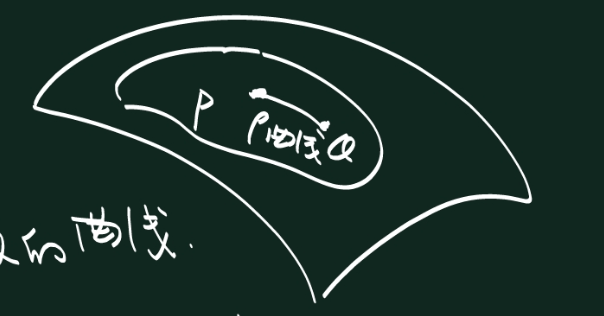
\includegraphics[width=0.48\textwidth]{fig1.png} % 图片宽度略小于环境宽度
    \end{figure}
    \[
    \frac{dr}{ds} = r_{\rho} \cdot \frac{d\rho}{ds} + r_{\theta} \cdot \frac{d\theta}{ds}
    \]
    \[
    \Rightarrow \left| \frac{dr}{ds} \right| = \sqrt{\left( \frac{d\rho}{ds} \right)^2 + G \left( \frac{d\theta}{ds} \right)^2}
    \]
    \[
    I = d\rho \otimes d\rho + G \, d\theta \otimes d\theta.
    \]
    
    故而
    \[
    L(r) = \int_0^1 \left| \frac{dr}{ds} \right| ds = \int_0^1 \sqrt{\left( \frac{d\rho}{ds} \right)^2 + G \left( \frac{d\theta}{ds} \right)^2} ds \geq \int_0^1 d\rho = \rho_0.
    \]
    \item 设 \( r \) 不完全落在 \( U \) 中,
    \begin{figure}[h]
        \centering
        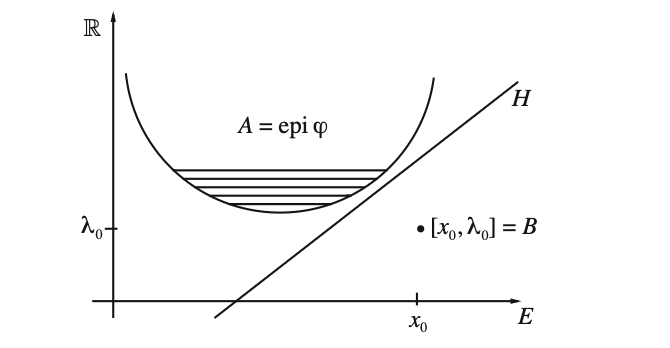
\includegraphics[width=0.48\textwidth]{fig2.png} % 图片宽度略小于环境宽度
    \end{figure}
    
    则
    \[
    \exists R \in \partial U, \text{ 使得 } r \text{ 通过 } R.
    \]
    容易看出 \( L(r) \geq L(\widehat{PR}) \geq L(\overline{C}) \)
\end{enumerate}
\end{proof}

\chapter{曲面的整体性质}
\section{测地三角形的Gauss公式}
\begin{figure}[h]
    \centering
    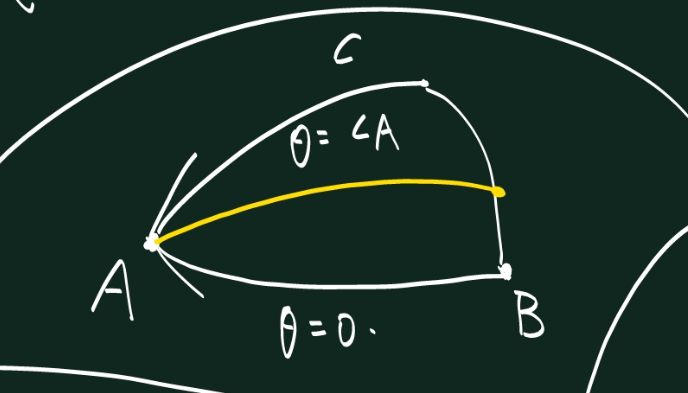
\includegraphics[width=0.48\textwidth]{fig3.png} % 图片宽度略小于环境宽度
\end{figure}
\begin{theorem}
    我们称 $\triangle ABC$ 为一个测地三角形,若
\begin{enumerate}
    \item 三条弧均存在于以 $A$ 为顶点的测地极坐标系中,且都是测地线。
    \item $\widehat{AB}$ 对应于 $\theta = 0$,$\widehat{AC}$ 对应于 $\theta = \angle A$。
    \item $\widehat{BC}$ 也是测地线。
\end{enumerate}

则
\[
\int_{\triangle ABC} K d\sigma = \angle A + \angle B + \angle C - \pi.
\]
\end{theorem}

\textbf{特例 1} 曲面为平面。
\[
K \equiv 0, \text{ 公式} \Leftrightarrow \angle A + \angle B + \angle C = \pi.
\]

\textbf{特例 2} 曲面为球面。
若半径为 \( R \),\( K = \frac{1}{R^2} \)。
\begin{figure}[h]
    \centering
    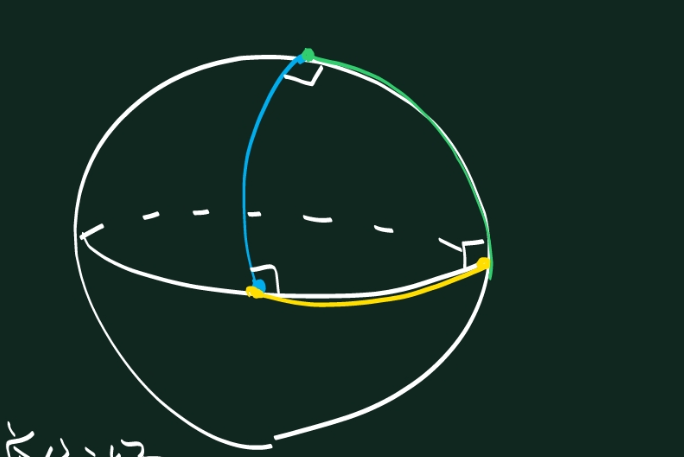
\includegraphics[width=0.48\textwidth]{fig4.png} % 图片宽度略小于环境宽度
\end{figure}

左
\[
 \int_{\triangle ABC} K d\sigma = \frac{1}{R^2} \int_{\triangle ABC} d\sigma = \frac{1}{R^2} S_{\triangle ABC}= \frac{1}{R^2} \cdot \frac{1}{2} (4\pi R^2) = \frac{\pi}{2}.
\]

右:\(\angle A + \angle B + \angle C - \pi = \pi\)($\angle A , \angle B ,  \angle $C都是 \(\pi/2\))。

\[
\angle A + \angle B + \angle C - \pi = \pi \Rightarrow \angle A + \angle B + \angle C - \pi = S_{\triangle ABC}.
\]
\begin{proof}
    注意到在测地极坐标系下,
\[
I = d\rho \otimes d\rho + G \, d\theta \otimes d\theta, \quad K = -\frac{(\sqrt{G})_{\rho\rho}}{\sqrt{G}}.
\]
\[
d\sigma = \sqrt{EG - F^2} \, d\rho \, d\theta = \sqrt{G} \, d\rho \, d\theta.
\]
故而 左边 \(= \int_{\triangle ABC} K \, d\sigma = \int_0^{\angle A} \left[ \int_0^{BC} -\frac{(\sqrt{G})_{\rho\rho}}{\sqrt{G}} \cdot \sqrt{G} \, d\rho \right] d\theta\)
\[
= \int_0^{\angle A} -(\sqrt{G})_{\rho \big|_{BC}} \bigg|_0^{\rho} \, d\theta. \quad (\text{注意到} \lim_{\rho \to 0} (\sqrt{G})_{\rho} = 1)
\]
\[
= \int_0^{\angle A} \left[ 1 - (\sqrt{G})_{\rho \big|_{BC}} \right] d\theta = \angle A - \int_0^{\angle A} (\sqrt{G})_{\rho \big|_{BC}} \, d\theta.
\]

\begin{wrapfigure}{r}{0.5\textwidth} % r: 图片右对齐;0.5\textwidth: 图片宽度
    \centering
    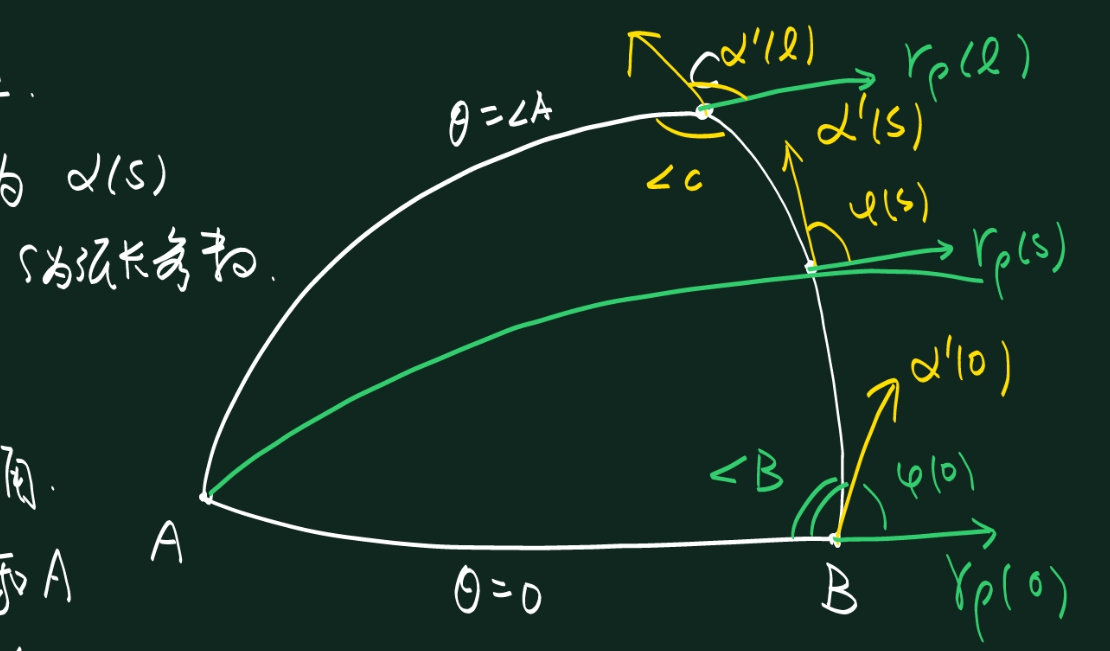
\includegraphics[width=0.48\textwidth]{fig5.png} % 图片宽度略小于环境宽度
   \end{wrapfigure}

  注意到 $\widehat{BC}$ 仍然在曲面上。

故而 $\widehat{BC}$ 可参数化为 $\alpha(s) = r(\rho(s), \theta(s))$。其中 $s$ 为弧长参数。

定义 $\varphi(s)$ 是 $\alpha'(s)$ 和 $\gamma_\rho(s)$ 的夹角。

其中 $r_\rho(s)$ 为 $\alpha(s)$ 和 $A$ 之间的 $\rho-$ 曲线的单位切向。

\textbf{FACT} 假设 $\widehat{BC}$ 弧长为 $\ell$.

\begin{enumerate}
    \item $\varphi(0) = \pi - \angle B.$
    \item $\varphi(\ell) = \angle C.$
    \item $\varphi$ 关于 $S$ 可微
    \item $\cos \varphi(s) = \alpha'(s) \cdot \gamma_{\rho}(s)$
    \item $\sin \varphi(s) = \alpha'(s) \cdot \gamma_{\theta}(s) / \sqrt{g}.$
\end{enumerate}
故下证
\[
\int_0^{\angle A}   - (\sqrt{G})_{\rho}  \bigg|_{BC} d\theta = \int_0^{\ell} -(\sqrt{G})_ {\rho} \frac{d\theta}{ds} ds = \int_0^{\ell} \frac{d\varphi}{ds} ds \tag{*}
\]

对(4)关于 $s$ 求导
\begin{align*}
    -\sin \varphi(s) \cdot \frac{d\varphi}{ds} &= \alpha'(s) \cdot r_{\rho}(s) + \alpha'(s) \cdot \frac{d}{ds} r_{\rho}(s).\\
    &= \alpha'(s) \cdot \frac{d}{ds} r_{\rho}(\rho(s), \theta(s))\\
    &=\left( r_{\rho} \frac{d\rho}{ds} + r_{\theta} \frac{d\theta}{ds} \right) \cdot \left( r_{\rho\rho} \frac{d\rho}{ds} + r_{\rho\theta} \frac{d\theta}{ds} \right).
\end{align*}


注意到$\quad |r_\rho| = 1 \iff r_\rho \cdot r_\rho = 1 \Rightarrow 
\begin{cases}
r_\rho \cdot r_{\rho\rho} = 0 \\
r_\rho \cdot r_{\rho\theta} = 0
\end{cases}$
\[
r_\theta \cdot r_{\rho\rho} = (r_\theta \cdot r_\rho)_{\rho\rho} - r_{\rho\theta} \cdot r_\rho = 0
\]

\[
\Rightarrow -\sin\varphi(s) \frac{d^2 \varphi}{ds^2} = r_\theta \cdot r_\rho \left( \frac{d\theta}{ds} \right)^2 = \frac{1}{2} G_\rho \left( \frac{d\theta}{ds} \right)^2
\]

\[
\text{但同时} \quad \sin\varphi(s) = \alpha'(s) \cdot \frac{r_\theta}{\sqrt{G}} = \left( r_\rho \frac{d\rho}{ds} + r_\theta \frac{d\theta}{ds} \right) \cdot \frac{r_\theta}{\sqrt{G}} = \sqrt{G} \left( \frac{d\theta}{ds} \right)
\]

\[
\Rightarrow \frac{d\varphi}{ds} = -\frac{G_\rho}{2\sqrt{G}} \left( \frac{d\theta}{ds} \right) = -\left( \sqrt{G} \right)_\rho \left( \frac{d\theta}{ds} \right)
\]
回带*即可证得


\end{proof}
\begin{remark}
    事实上 Gauss 测地三角形公式的 $\angle A, \angle B, \angle C$ 相应换成外角.
\end{remark}
\begin{definition}[外角]
    记
$$
\begin{cases}
\theta_1 = \pi - \angle A \\
\theta_2 = \pi - \angle B \\
\theta_3 = \pi - \angle C
\end{cases}
\quad \text{为对应的外角.}
$$
\end{definition}
公式改写为
\begin{align*}
\int_{\triangle ABC} K d\sigma &= \angle A + \angle B + \angle C - \pi \\
&= (\pi - \theta_1) + (\pi - \theta_2) + (\pi - \theta_3) - \pi
\end{align*}

$$
\iff \boxed{\int_{\triangle ABC} K d\sigma + \sum_{i=1}^{3} \theta_i = 2\pi}
$$

\begin{remark}
    平面三角形的内角和为$\pi$是"偶然"的.

四边形内角和 $\to 2\pi$

$n$边形内角和 $\to (n-2)\pi$

但所有$n$边形外角和总是 $n\pi - (n-2)\pi = 2\pi$.

故而 Gauss 定理是在说
$$ \int_{\triangle ABC} K d\sigma + \text{外角和} = 2\pi. $$
\end{remark}

我们想推广 Gauss 定理到多边形.
\begin{definition}[分段光滑简单闭合曲线)]
    $$ \alpha: [0, l] \to S $$
连续曲线满足:
\begin{enumerate}
    \item $\alpha(0) = \alpha(l)$
    \item 若 $S_1 \neq S_2$, $S_1, S_2 \in [0, l)$, 则 $\alpha(S_1) \neq \alpha(S_2)$
    \item 存在一个 $[0, l]$ 的分割 $0=t_0 < \dots < t_k = l$, 使得 $\alpha(t)$ 在 $[t_{i-1}, t_i]$ 上都光滑. (即 $t=t_i$ 处可能有外角)
\end{enumerate}
\end{definition}
\begin{figure}[h]
    \centering
    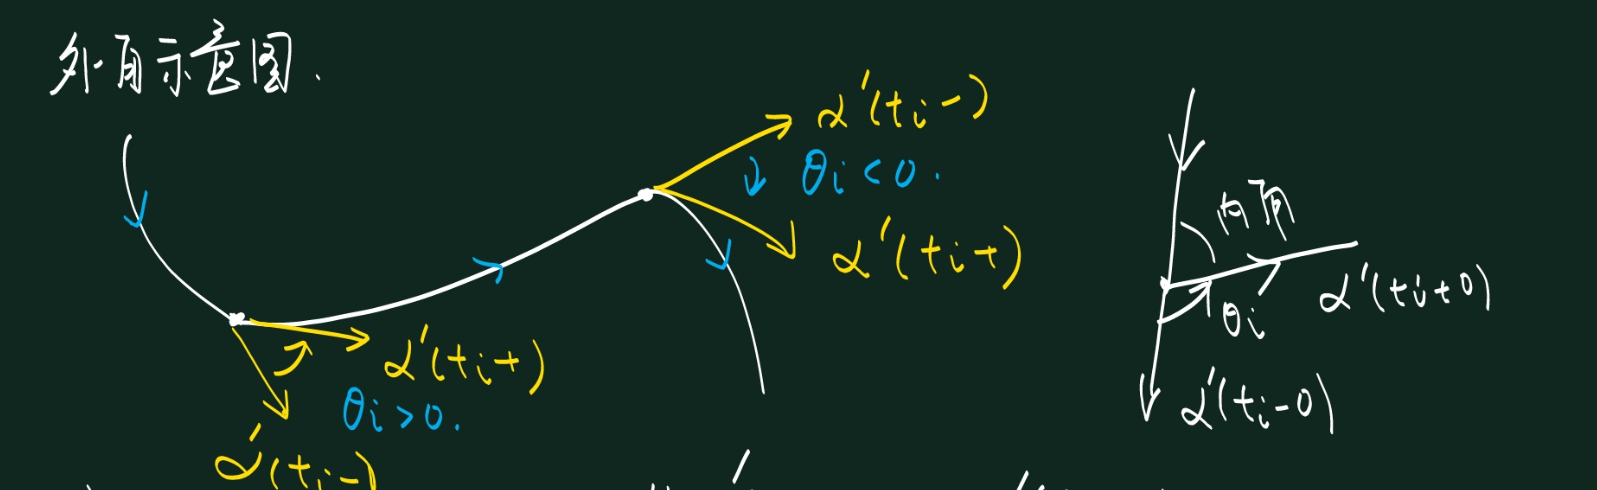
\includegraphics[width=0.6\textwidth]{fig6.png} % 图片宽度略小于环境宽度
\end{figure}
\begin{definition}[外角]
    我们规定,若 $\alpha'(t_i-0) \ne \alpha'(t_i+0)$,从 $\alpha'(t_i-0)$ 到 $\alpha'(t_i+0)$ 逆时针定向成外角 $\theta_i$.

\textbullet \ $-\pi \le \theta_i \le \pi$. (对于三角形外角的一种推广).
\end{definition}

Bonnet 推广了 Gauss 定理, 将其中测地线的要求去掉!
\section{Gauss - Bonnet 定理, 局部版本}
\begin{theorem}
    假设 $C$ 为曲面 $S$ 上一条分段光滑、简单闭曲线,
其所围成的区域为 $D$, $C$ 上的外角记为 $\theta_i$, 则
$$ \iint_D K d\sigma + \oint_C k_g ds + \sum_{i=1}^n \theta_i = 2\pi. $$
\end{theorem}

Step 1 假设 D 是足够小, 能包含在 P 的一个参数邻域, 使得 D 可以嵌入以 P 为中心的正交参数网。

由于 F=0, 可套用 Liouville 公式:
$$
\begin{cases}
\frac{du}{ds} = \frac{\cos\theta}{\sqrt{E}} \\
\frac{dv}{ds} = \frac{\sin\theta}{\sqrt{G}}
\end{cases}
$$

$$
\oint_C k_g ds = \oint_C \left( \frac{d\theta}{ds} + \frac{1}{2\sqrt{E}\sqrt{G}} \frac{G_u}{\sqrt{G}} \sin\theta - \frac{1}{2\sqrt{G}} \frac{E_v}{\sqrt{E}} \cos\theta \right) ds
$$
$$
= \oint_C d\theta + \oint_C - \frac{1}{2\sqrt{G}} \left( \frac{E_v}{\sqrt{E}} \right) \sqrt{E} du + \frac{1}{2\sqrt{E}} \frac{G_u}{\sqrt{G}} \sqrt{G} dv
$$
$$
= \oint_C d\theta + \oint_C - \left( \frac{(\sqrt{E})_v}{\sqrt{G}} \right) du + \left( \frac{(\sqrt{G})_u}{\sqrt{E}} \right) dv
$$

D 为单连通区域, 故可用 Green 公式:
$$ \oint_C P du + Q dv = \iint_D (Q_u - P_v) du dv $$
$$ \Rightarrow \oint_C k_g ds = \oint_C d\theta + \iint_D \left\{ \left( \frac{(\sqrt{G})_u}{\sqrt{E}} \right)_u + \left( \frac{(\sqrt{E})_v}{\sqrt{G}} \right)_v \right\} du dv $$
记 Gauss 曲率为 $K = -\frac{1}{\sqrt{EG}} \left\{ \left( \frac{(\sqrt{E})_v}{\sqrt{G}} \right)_v + \left( \frac{(\sqrt{G})_u}{\sqrt{E}} \right)_u \right\}$。
当 F=0,
$$ \oint_C d\theta - \iint_D K d\sigma \quad \text{其中 } d\sigma = \sqrt{EG} du dv $$
$$ \Rightarrow \iint_D K d\sigma + \oint_C k_g ds = \oint_C d\theta \quad \leftarrow \text{局部情形} $$
其中 $\oint_C d\theta = \theta(l) - \theta(0)$。

\begin{figure}[h]
    \centering
    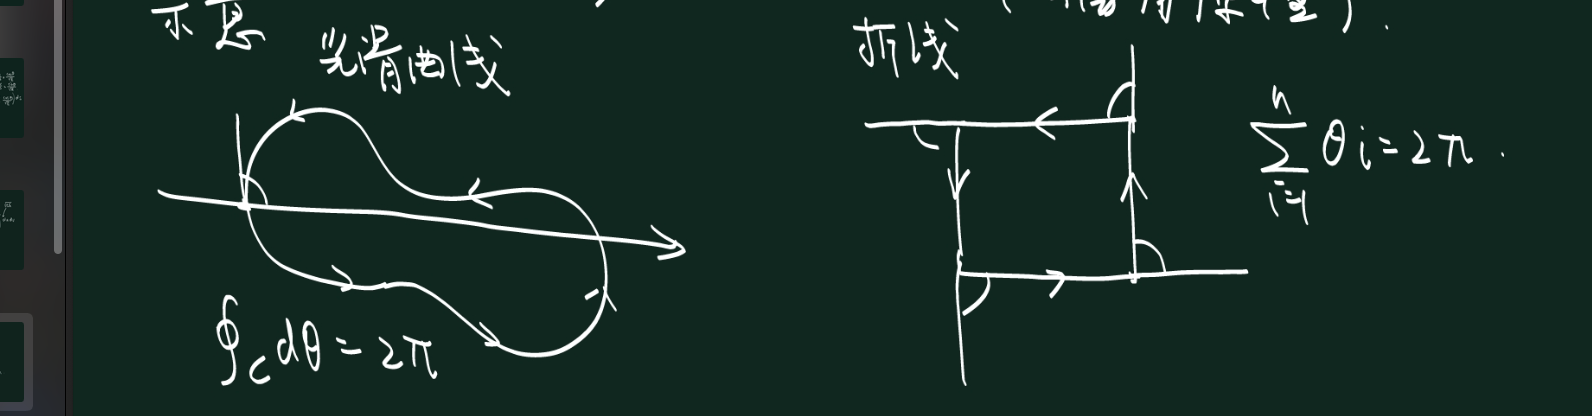
\includegraphics[width=0.6\textwidth]{fig7.png} % 图片宽度略小于环境宽度
\end{figure}


Step 2 证明: Gauss-Bonnet 对可剖分曲面成立。

\begin{figure}[h]
    \centering
    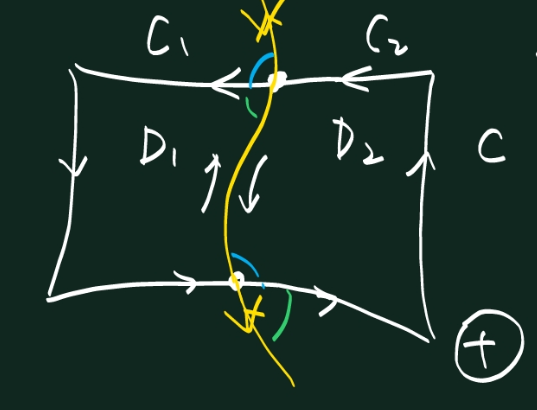
\includegraphics[width=0.6\textwidth]{fig8.png} % 图片宽度略小于环境宽度
\end{figure}


假设对于 $D_1, D_2$, Gauss-Bonnet 成立
$$ \iint_{D_1} K d\sigma + \oint_{C_1} k_g ds + \sum_{i=1}^{4} \tilde{\theta}_i = 2\pi $$
$$ \iint_{D_2} K d\sigma + \oint_{C_2} k_g ds + \sum_{i=5}^{8} \tilde{\theta}_i = 2\pi $$
相加
$$ \Rightarrow \iint_{D} K d\sigma + \oint_{C} k_g ds + \sum_{i=1}^{8} \tilde{\theta}_i = 4\pi $$
$$ \Rightarrow \iint_{D} K d\sigma + \oint_{C} k_g ds + \sum_{i=1}^{4} \theta_i = 2\pi \quad  $$
相邻两区域的外角互补为 $2\pi$。

从而
$$ \iint_D K d\sigma + \oint_C k_g ds + \sum \theta_i = \oint_C d\theta + \sum \theta_i = 2\pi $$
\section{Gauss-Bonnet定理整体性质}
\begin{definition}[三角剖分]
    对于正则曲面 S, 三角剖分是一族曲边三角形 $\{T_\alpha\}$ 满足以下要求:
\begin{enumerate}
    \item $\bigcup_{\alpha} T_\alpha = S$.
    \item $\forall p \in S$, $p$ 只能有以下几种可能:
    \begin{enumerate}
        \item 存在唯一的 $T_\alpha$, 使 $p$ 在 $T_\alpha$ 内部.
        
        \item 若 $p$ 在某个 $T_1$ 的棱上 (即不在顶点上), 则 $p$ 至多再属于一个 $T_2$ 的棱. 且 $p$ 落在 $T_1 \cup T_2$ 的内部.
        
        \item 若 $p$ 落在某个 $T_\alpha$ 的顶点上, 则 $p$ 至多落在有限个三角形的共同顶点上. 且这些三角形两两之间至多一条公共边.
        
    \end{enumerate}
\end{enumerate}

\end{definition}

\begin{figure}[H]
\centering
\begin{minipage}{0.48\textwidth}
    \centering
    \begin{tikzpicture}
        % 曲面片
        \draw (0,0) .. controls (1,0.2) and (3, -0.2) .. (4,0);
        \draw (0,2) .. controls (1,2.2) and (3, 1.8) .. (4,2);
        \draw (0,0) -- (0,2);
        \draw (4,0) -- (4,2);
        
        % 曲边三角形
        \coordinate (A) at (1, 0.8);
        \coordinate (B) at (3, 1);
        \coordinate (C) at (2, 1.8);
        \draw (A) .. controls (2, 0.7) and (2.5, 0.8) .. (B);
        \draw (B) .. controls (2.8, 1.5) .. (C);
        \draw (C) .. controls (1.5, 1.6) .. (A);
        
        % 剖分线
        \foreach \i in {1,...,5} {
            \draw (A) -- (barycentric cs:A=0.3,B=0.35+\i*0.05,C=0.35-\i*0.05);
        }
        
        \node at (2.5, 1.6) {$T_i$};
    \end{tikzpicture}
    \caption{定义中的曲边三角形 $T_i$}
\end{minipage}
\hfill
\begin{minipage}{0.48\textwidth}
    \centering
    \begin{tikzpicture}
        % Case 2: p 在棱上
        \draw (0,0) node[below] {$T_1$} -- (2,1) node[label={[label distance=-2pt]45:$P$}] {$\cdot$} -- (0,2) -- cycle;
        \draw (2,1) -- (4,0) -- (4,2) -- cycle;
        \node at (3.5, 1) {$T_2$};
    \end{tikzpicture}
    \caption{情形 (2): 点 P 位于公共棱上}
    
    \vspace{1cm}
    
    \begin{tikzpicture}
        % Case 3: p 在顶点上
        \coordinate (P) at (0,0);
        \node[below left] at (P) {$P$};
        \draw (P) -- (2,0) -- (1.5, 1) -- cycle;
        \node at (1.2, 0.4) {$T_1$};
        \draw (P) -- (1.5, 1) -- (0, 1.8) -- cycle;
        \node at (0.5, 1) {$T_2$};
        \draw (P) -- (0, 1.8) -- (-1, 1.2) -- cycle;
        \node at (-0.5, 1.2) {$T_3$};
        \draw (P) -- (-1, 1.2) -- (-1.5, 0) -- cycle;
        \node at (-1, 0.4) {$T_4$};
        \node at (-0.5, -0.5) {$\dots$};
    \end{tikzpicture}
    \caption{情形 (3): 点 P 为公共顶点}
\end{minipage}
\end{figure}

\begin{theorem}
     紧曲面一定可被有限个三角剖分
\end{theorem}

\begin{figure}[htbp]
    \centering
    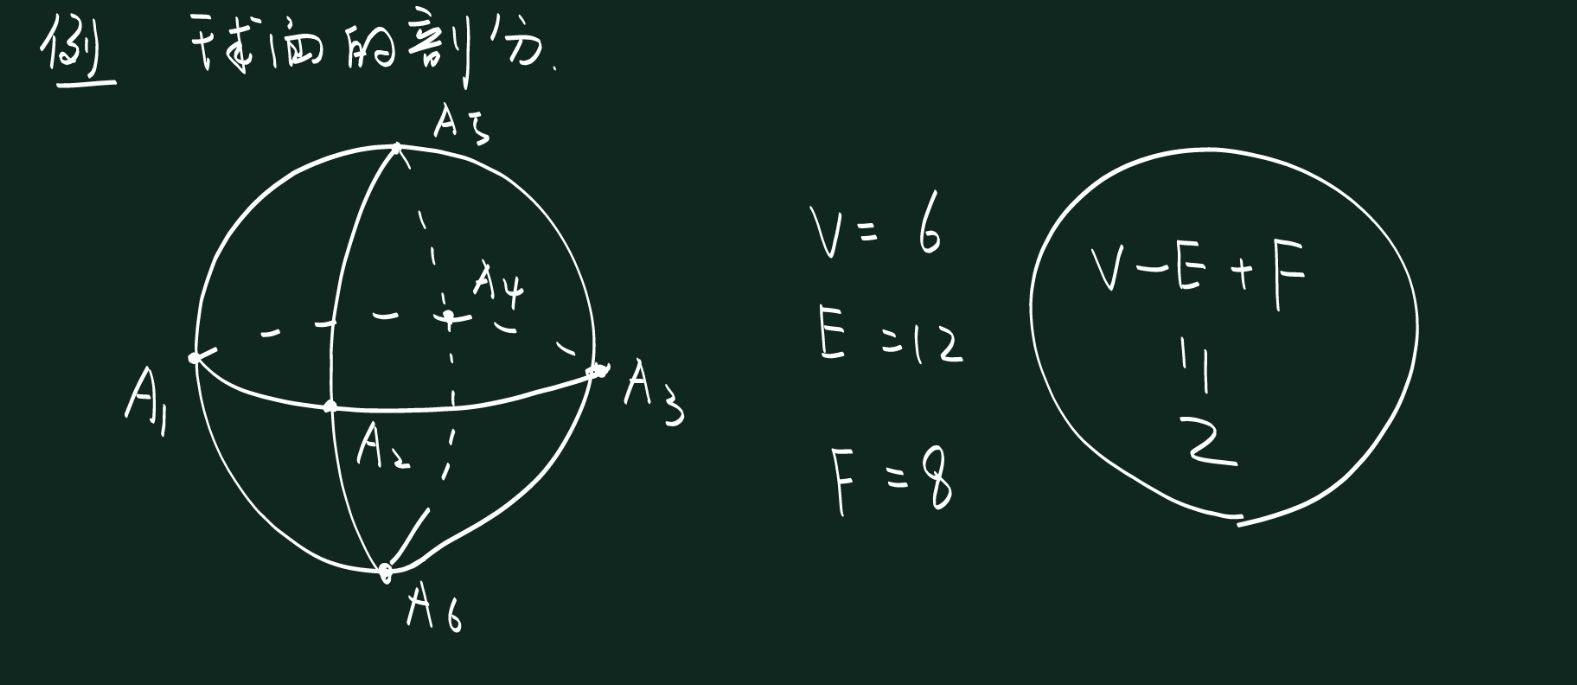
\includegraphics[width=0.6\textwidth]{fig9.png} % 图片宽度略小于环境宽度
\end{figure}

\begin{figure}[htbp]
    \centering
    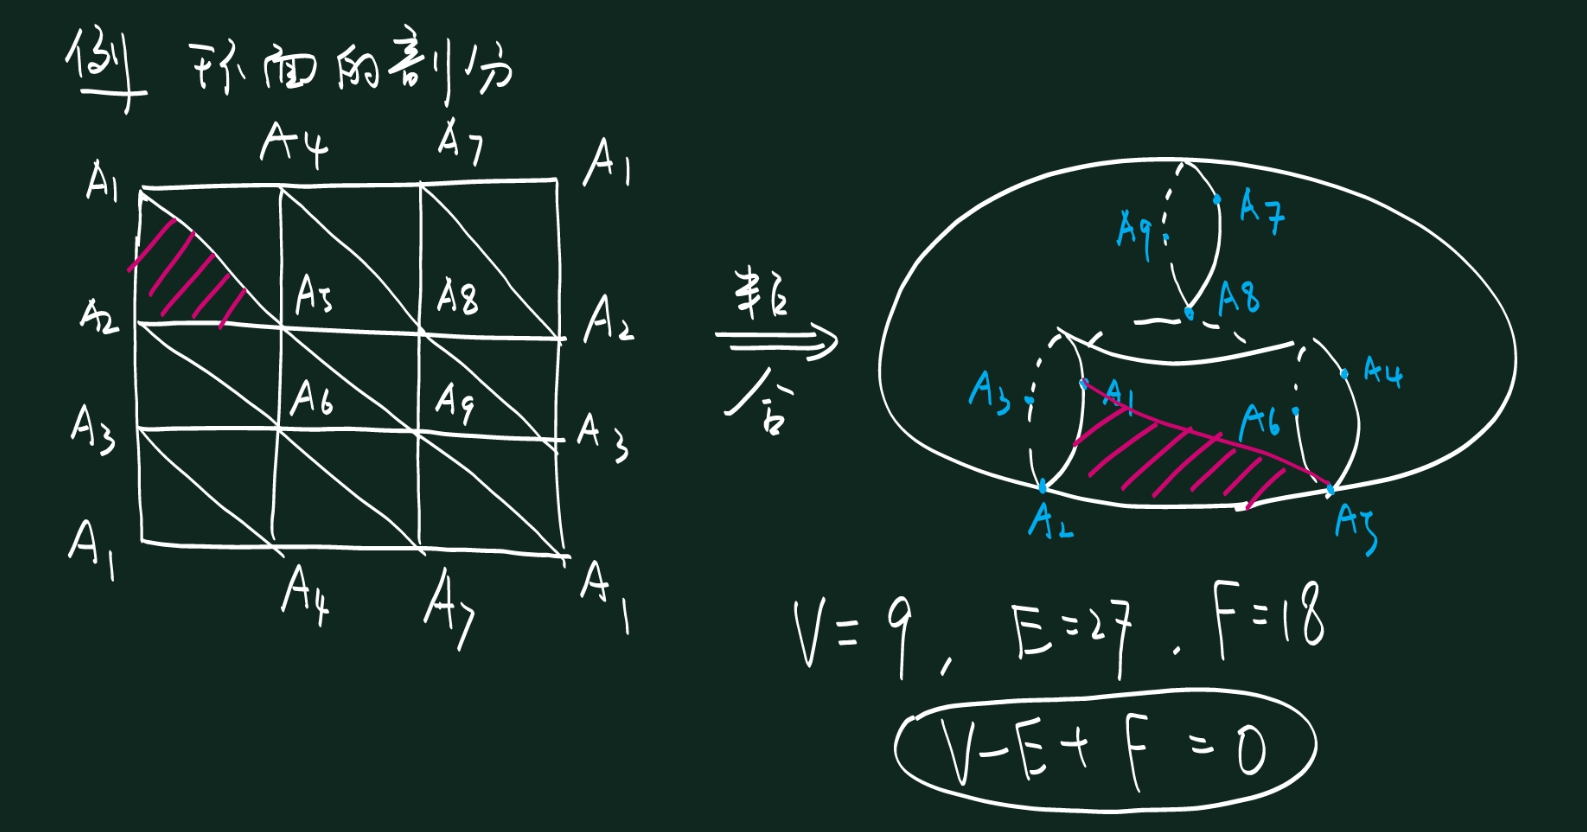
\includegraphics[width=0.6\textwidth]{fig10.png} % 图片宽度略小于环境宽度
\end{figure}

\begin{definition}[欧拉示性数]
    若曲面 S 可被有限三角剖分, 则定义
$$ \chi(S) = V-E+F $$
称其为曲面的欧拉示性数。
\end{definition}
\underline{事实.} 欧拉示性数是拓扑不变量,
即若存在 $S_1 \xrightarrow{\text{h}} S_2$ 拓扑同胚, 则 $\chi(S_1) = \chi(S_2)$。
对于紧致曲面 $\chi(S)=2-2g$, g 称为亏格 (洞的个数)。

利用三角剖分和欧拉示性数, 我们可以给出 Gauss-Bonnet 整体版本。
\begin{theorem}[Gauss-Bonnet 整体版本]
    设 S 为紧致无边曲面, 则
$$ \iint_S K d\sigma = 2\pi\chi(S) = 2\pi(V-E+F) $$
$$ \text{分析} \qquad \text{拓扑} $$
\end{theorem}
\begin{proof}


根据 Radó 定理,紧致曲面 S 可被有限个(设为 F 个)曲边三角形 $\{T_i\}_{i=1}^F$ 进行剖分。

对于其中任意一个曲边三角形 $T_i$,我们应用局部 Gauss-Bonnet 公式(包含外角的形式):
$$\iint_{T_i} K d\sigma + \oint_{\partial T_i} k_g ds + \sum_{j=1}^{3} \theta_{ij} = 2\pi$$
其中 $\oint_{\partial T_i} k_g ds$ 是沿 $T_i$ 边界的测地曲率积分,$\theta_{ij}$ 是 $T_i$ 在其第 $j$ 个顶点的外角。

将这 F 个三角形的公式全部相加,我们得到:
$$\sum_{i=1}^{F} \left( \iint_{T_i} K d\sigma \right) + \sum_{i=1}^{F} \left( \oint_{\partial T_i} k_g ds \right) + \sum_{i=1}^{F} \sum_{j=1}^{3} \theta_{ij} = \sum_{i=1}^{F} 2\pi$$



我们分别处理上式左侧的三项:
\begin{enumerate}
    \item \textbf{高斯曲率积分项}: 所有小三角形上的面积分之和,自然就是整个曲面 S 上的面积分。
    $$\sum_{i=1}^{F} \iint_{T_i} K d\sigma = \iint_S K d\sigma$$
    \item \textbf{测地曲率积分项}: 因为曲面 S 没有边界,所以三角剖分中的每一条棱都必然是两个相邻三角形的公共边。在对这两个相邻三角形进行环路积分时,这条公共棱的路径方向正好相反。因此,沿这条棱的测地曲率积分大小相等、符号相反,两者相加恰好为零。这个“边相抵消”的现象作用于所有内部棱,故:
    $$\sum_{i=1}^{F} \oint_{\partial T_i} k_g ds = 0$$
    \item \textbf{外角和项}: 我们首先将外角 $\theta_{ij}$ 用其对应的内角 $\alpha_{ij}$ 表示,即 $\theta_{ij} = \pi - \alpha_{ij}$。
    $$\sum_{i=1}^{F} \sum_{j=1}^{3} \theta_{ij} = \sum_{i=1}^{F} \sum_{j=1}^{3} (\pi - \alpha_{ij})$$
    总共有 F 个三角形,每个有 3 个角,因此上式变为:
    $$= 3F\pi - \sum_{i,j} \alpha_{ij}$$
    这里的 $\sum \alpha_{ij}$ 指所有 F 个三角形的内角总和。我们可以换个角度来计算这个总和:按顶点(Vertex)来加。因为 S 是一个正则曲面,汇集在 V 个顶点中任意一个顶点周围的所有内角之和都恰好是 $2\pi$。因此,所有内角的总和就是:
    $$\sum_{i,j} \alpha_{ij} = \sum_{v=1}^{V} (\text{汇集在顶点 v 的内角和}) = 2\pi V$$
    所以,总的外角和为:
    $$\sum_{i=1}^{F} \sum_{j=1}^{3} \theta_{ij} = 3F\pi - 2V\pi$$
\end{enumerate}


将简化后的各项代入第一步的总公式中:
$$\iint_S K d\sigma + 0 + (3F\pi - 2V\pi) = 2F\pi$$
移项整理可得:
$$\iint_S K d\sigma = 2F\pi - (3F\pi - 2V\pi) = 2V\pi - F\pi$$
为了引入棱数 E,我们使用一个重要的组合拓扑恒等式。在三角剖分中,每个三角形有 3 条棱,而每条棱又被 2 个三角形共享,因此棱数 E 和面数 F 的关系为:
$$2E = 3F$$
现在,我们将这个关系代入上式。为了凑出 $V-E+F$ 的形式,我们进行如下代数变换:
\begin{align*}
\iint_S K d\sigma &= 2\pi V - F\pi \\
&= 2\pi V - (3F - 2F)\pi \\
&= 2\pi V - (2E - 2F)\pi \quad (\text{因为 } 3F=2E) \\
&= 2\pi V - 2\pi E + 2\pi F \\
&= 2\pi (V - E + F)
\end{align*}



最终我们得到:
$$\iint_S K d\sigma = 2\pi \chi(S)$$
\end{proof}
\end{document}
